\documentclass[a4paper,11pt]{article}
\pdfoutput=1
\usepackage{jinstpub} % for details on the use of the package,                           please
                     % see the JINST-author-manual
\usepackage{xcolor,soul,framed} %,caption
\usepackage{graphicx}
\usepackage{subcaption}
\usepackage{wrapfig}
\usepackage{mdwmath}
\usepackage{mdwtab}
\usepackage{eqparbox}
\usepackage{url}
\usepackage{dblfloatfix}    % To enable figures at the bottom of page
%\usepackage{kantlipsum}     % for random text
\usepackage{hyperref}
\usepackage[export]{adjustbox}
% \usepackage{longtable}
% \usepackage{booktabs}
% \usepackage{csvsimple}
% longtable support required by pandoc >1.10

%--------------------------------------------------------------------------------%
%%%%%%%%%%%%%%%%%%%%%%%%%%%%%% Document Start %%%%%%%%%%%%%%%%%%%%%%%%%%%%%%%%%%%%
%--------------------------------------------------------------------------------%

\begin{document}
%\bstctlcite{IEEEexample:BSTcontrol}
    \title{Contaminate Imaging in Chicken Using CZT Detector}
    
\author[a,1]{Jericho~O'Connell,\note{Corresponding author.}}
\author[a]{Kevin J. Murphy}
\author[a]{Spencer M. Robinson}
\author[b]{Kris~Iniewski}% <-this % stops a space
\author[a]{Magdalena~Bazalova-Carter}

\emailAdd{jerichoo@uvic.ca}

\affiliation[a]{University of Victoria,\\3800 Finnerty Rd, Victoria, BC, Canada}
\affiliation[b]{Redlen Technologies,\\123 - 1763 Sean Heights
Saanichton, BC, Canada}

%--------------------------------------------------------------------------------%
%%%%%%%%%%%%%%%%%%%%%%%%%%%%%% Abstract %%%%%%%%%%%%%%%%%%%%%%%%%%%%%%%%%%%%
%--------------------------------------------------------------------------------%

\abstract{
A 330 $\mu$m pitch  $8\times12$ Cadmium Zinc Telluride (CZT) detector with 6 energy bins is utilized to see potential benefits of its application in segmentation of soft tissue. Planar X-ray scans are completed using a table top set up consisting of a X-ray tube, and the CZT detector, both mounted on motion stages to allow for vertical and horizontal motion. A PMMA phantom with contaminates (glass, steel, plastic, polypropylene, and PFTE) was imaged as well as chicken flesh with contaminates (cartilage, bone, fat, plastic, wood, glass, rock, steel and aluminum) to determine there detectability given varying depths. These images were performed at 120 kVp, and 1 mA, with 1 second acquisition time. Given a Contrast to Noise Ratio (CNR) greater the 4 a computer is capable of accurately segmenting contaminates, this study looks to enquire about the potential of using Convolutional neural networks (CNN) to quickly sort flesh based on it components given the added detection ability capable with a multiple energy bin CZT detector.

}

\maketitle
% * <jericho.oconnell@icr.ac.uk> 2018-08-29T22:15:14.220Z:
%
% ^.

%--------------------------------------------------------------------------------%
%%%%%%%%%%%%%%%%%%%%%%%%%%%%%% Introduction %%%%%%%%%%%%%%%%%%%%%%%%%%%%%%%%%%%%
%--------------------------------------------------------------------------------%

\section{Introduction}




In this work we benchmark single, dual, and spectral imaging segmentation algorithms. We propose an out of the box two material segmentation algorithm that optimally segments based on five segmentation tasks. This is done using images acquired on a five energy bin CZT spectral imaging detector. Algorithms are benchmarked on a single, dual and spectral .



%Must add more paper that are being reference in this section: 	Papers about Airport Scanning, Jerichoos original simulations, Spectral Imaging of objects.


%--------------------------------------------------------------------------------%
%%%%%%%%%%%%%%%%%%%%%%%%% Materials/Methods %%%%%%%%%%%%%%%%%%%%%%%%%%%%%%%%%%%%
%--------------------------------------------------------------------------------%

\section{Materials and Methods}
\label{sec:methods}

\begin{figure}[htbp]

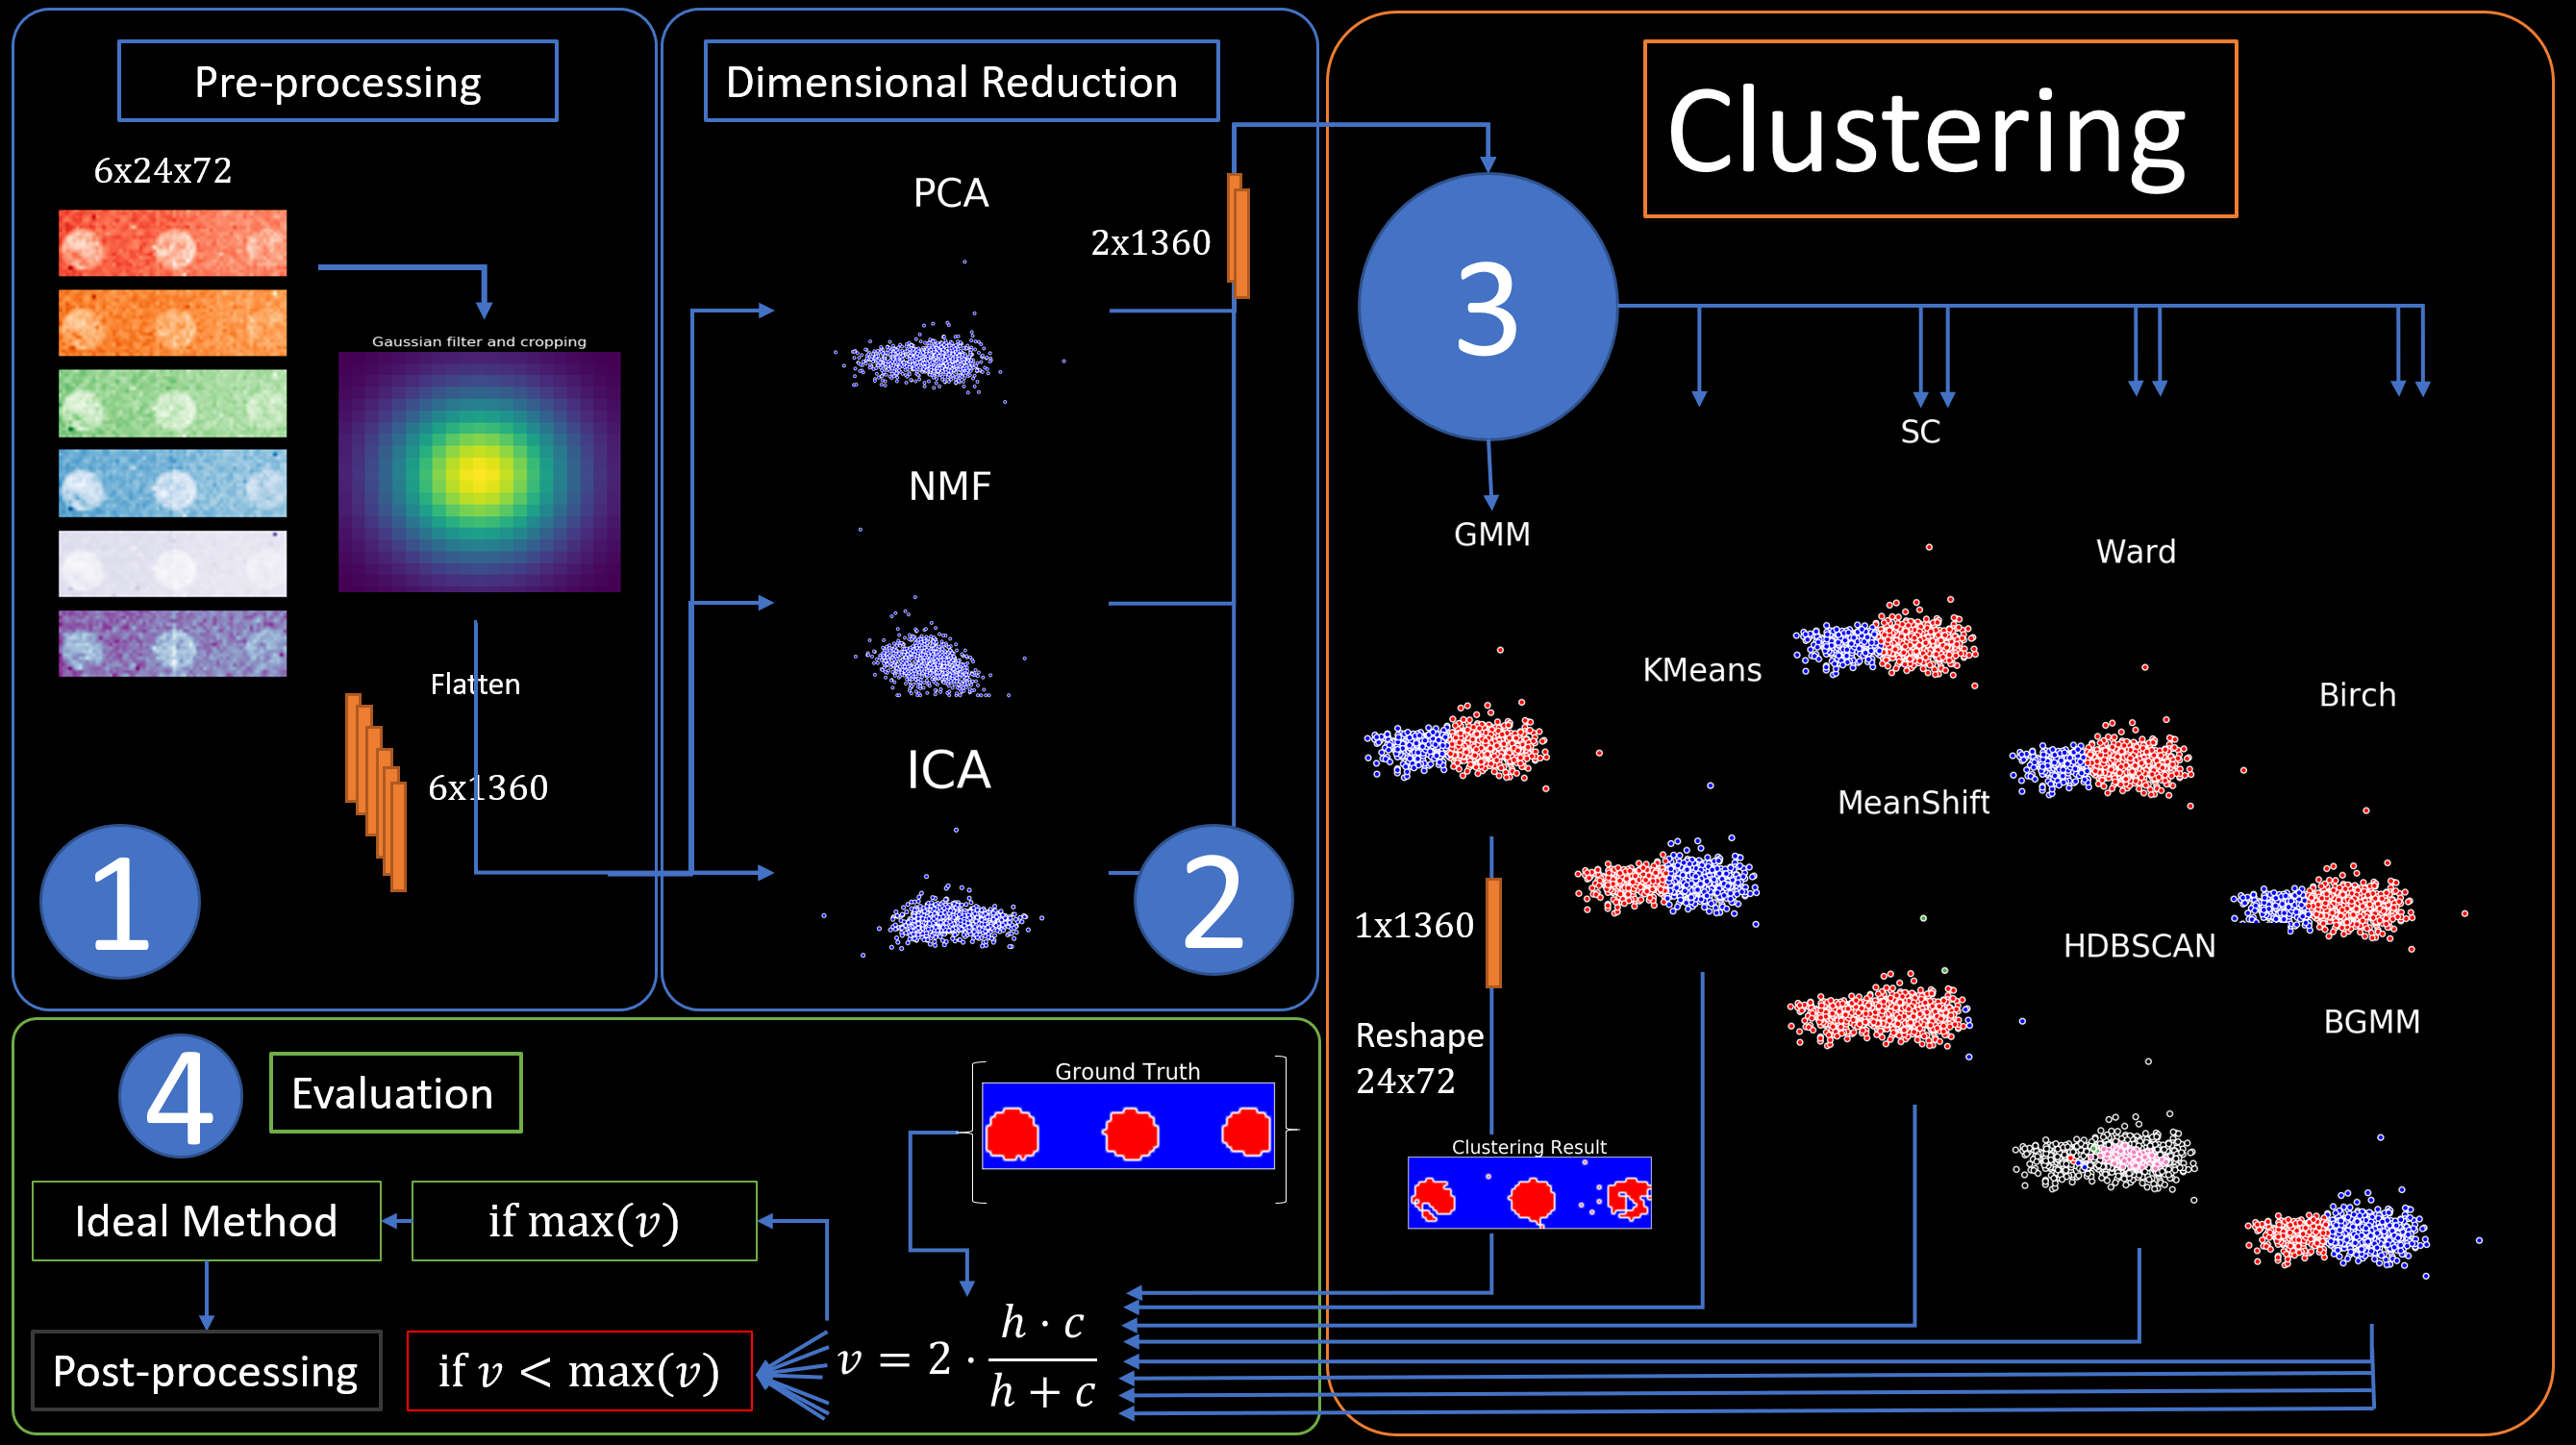
\includegraphics[width=\textwidth]{figures/flow_chart.png}

\caption{A general overview of the workflow is seen, outlining the four general steps of the segmentation method.}
\label{overview}
\end{figure}

\subsection{Data Aquistion}
X-ray scans were performed on a PMMA phantom with 5 contaminates (steel, glass, plastic, polypropylene, and PFTE) as well as chicken breast with various contaminates (bone, cartilage, fat, plastic, wood, glass, rock, steel, and aluminum).

Data was acquired using a CZT detector with a 8$\times$12 mm imaging array from Redlen Technologies. The 330 $\mu$m pitch high-flux CZT detector is 2mm thick and is able to operate at 250 $\frac{Mcps}{mm^2}$ without any signs of polarization. Travel Heat Method (THM) was adopted by Redlen Technologies when growing the CZT crystals used in the detector. These crystals were placed in a sensor that is connected to a photon counting ASIC which operates at rates of up to 62.5 $\frac{Mcps}{channel}$. This ASIC communicates with an external PC though LVDS I/Os via a programmable FPGA. The energies of photons incident with the detector are sorted into six energy bins by the ASIC. In the case of this experiment the energy bins were set to 16-33 keV, 33-41 keV, 41-50 keV, 50-90 keV, 90-120 keV, \& 120< keV.

The detector and X-ray source were both mounted on vertical and horizontal linear motion stages from Newport Corporations. These stages were oriented perpendicular to each other to allow for easy navigation while imaging the phantom, which was mounted between these two stages. The X-ray source used was a module XRS-160 from Comet Technologies. 

The PMMA phantom block as imaged in figure (1.C) was placed on the stage and the 3 smallest contaminates of each material were imaged. To image these contaminates each at different heights, the CZT detector and X-ray source were moved vertically in a uniform manner allowing for each material to be centered without any motion of the phantom block itself. Following the first round of data acquisitions a second block of 18mm PMMA was placed in front of the phantom block and images were acquired to determine the depth at which each contaminate could be visualized. 

In the case of the chicken flesh, each contaminate was able to fit in a phantom holder alongside the chicken. This block was placed on the stage and was able to be imaged in one scan per contaminate. 

Air scans were completed for each data acquisition and could then be processed using MATLAB (The Mathworks, Natick, MA) for image reconstruction and CNR calculations for each contaminate. During all scans the X-ray tube was using a cone beam operating at 1mA, 120 kV, with a 1mm focal spot. 


\begin{wrapfigure}{R}{0.5\textwidth}
  
  \begin{center}
    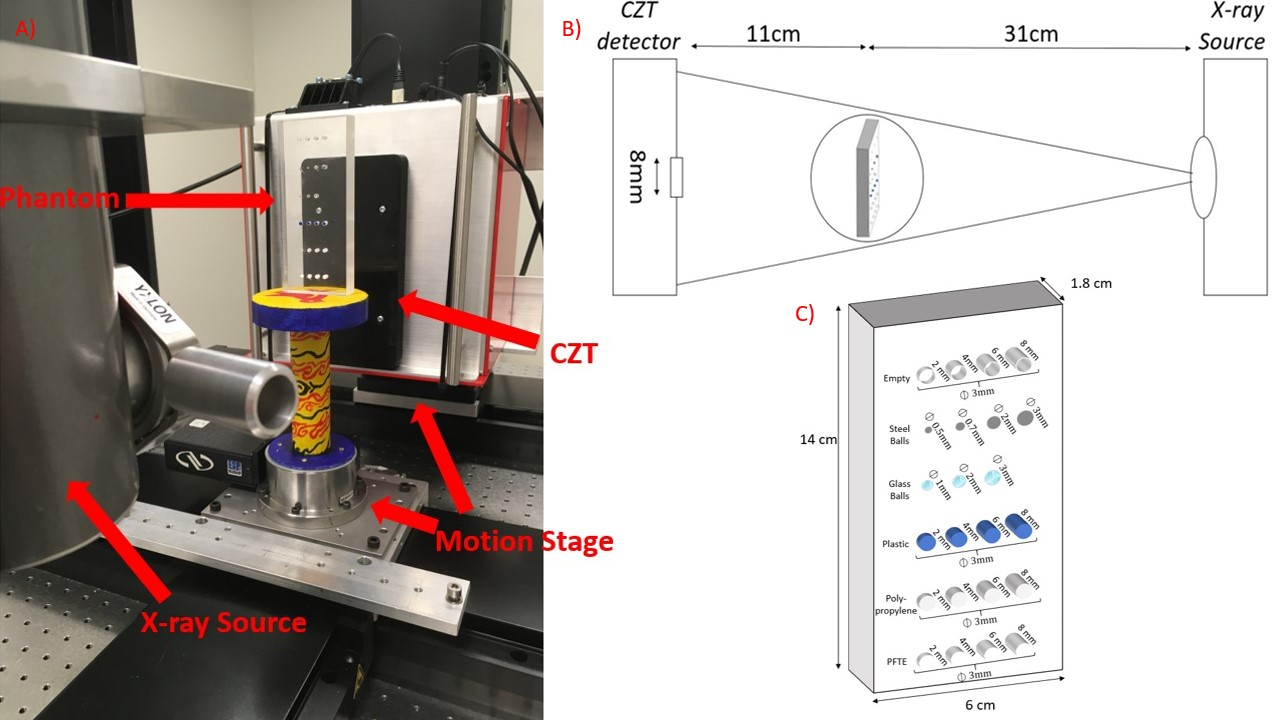
\includegraphics[width=0.48\textwidth]{FullFigure.jpg}
  \end{center}
  
  \caption{A) Shows an image of the lab after data was acquired with different components as labeled. B) Is a schematic of the lab with distances from source to detector labeled. C) The layout for the phantom used with sizes of contaminates as labeled.}
  
\end{wrapfigure}

\subsection{Image Segmentation}
\subsubsection{Overview}

Image segmentation is undertaken as a multistage process. A problem encountered is that regular X-ray imaging workflows are not designed to accommodate five or more dimensional spectral images. Here we borrow from the neighboring field of hyperspectral imaging, as images are multidimensional and clustering segmentation has been widely applied in the field \cite{Murphy2018UnsupervisedDiffusion,Gillis2012HyperspectralGraphs,Noe2001PartialClustering}. Mahesh et al. state that main steps in hyperspectral images segmentation include pre-processing of data, dimensional reduction, enhancement of spectral responses, and component detection or classification \cite{Mahesh2015HyperspectralMaterials}. These steps can also be seen in Figure \ref{overview}. Using this as an analog for spectral imaging similar methods are applied. An exception being the enhancement of spectral response as the modelling of the spectral response of the CZT detector is beyond the scope of this study.

\subsubsection{Pre-processing of Data}

After data aquisition, data pre-processing was performed using MATLAB 2017b (The MathWorks, Natick, USA). The images were first cropped to remove the highly non-uniform edge pixels in some parts of the detector. Dead pixels were then found manually and replaced with NaN values in the image. These NaN values were then interpolated to be the average of the surrounding eight pixels. The images were then smoothed using a two dimensional gaussian filter with a standard deviation of 0.5 as a preliminary method to reduce the noise in the image.

One can see the six input images after the initial pre-processing in Figure \ref{demonstrating_bins}

\begin{figure}[htbp]

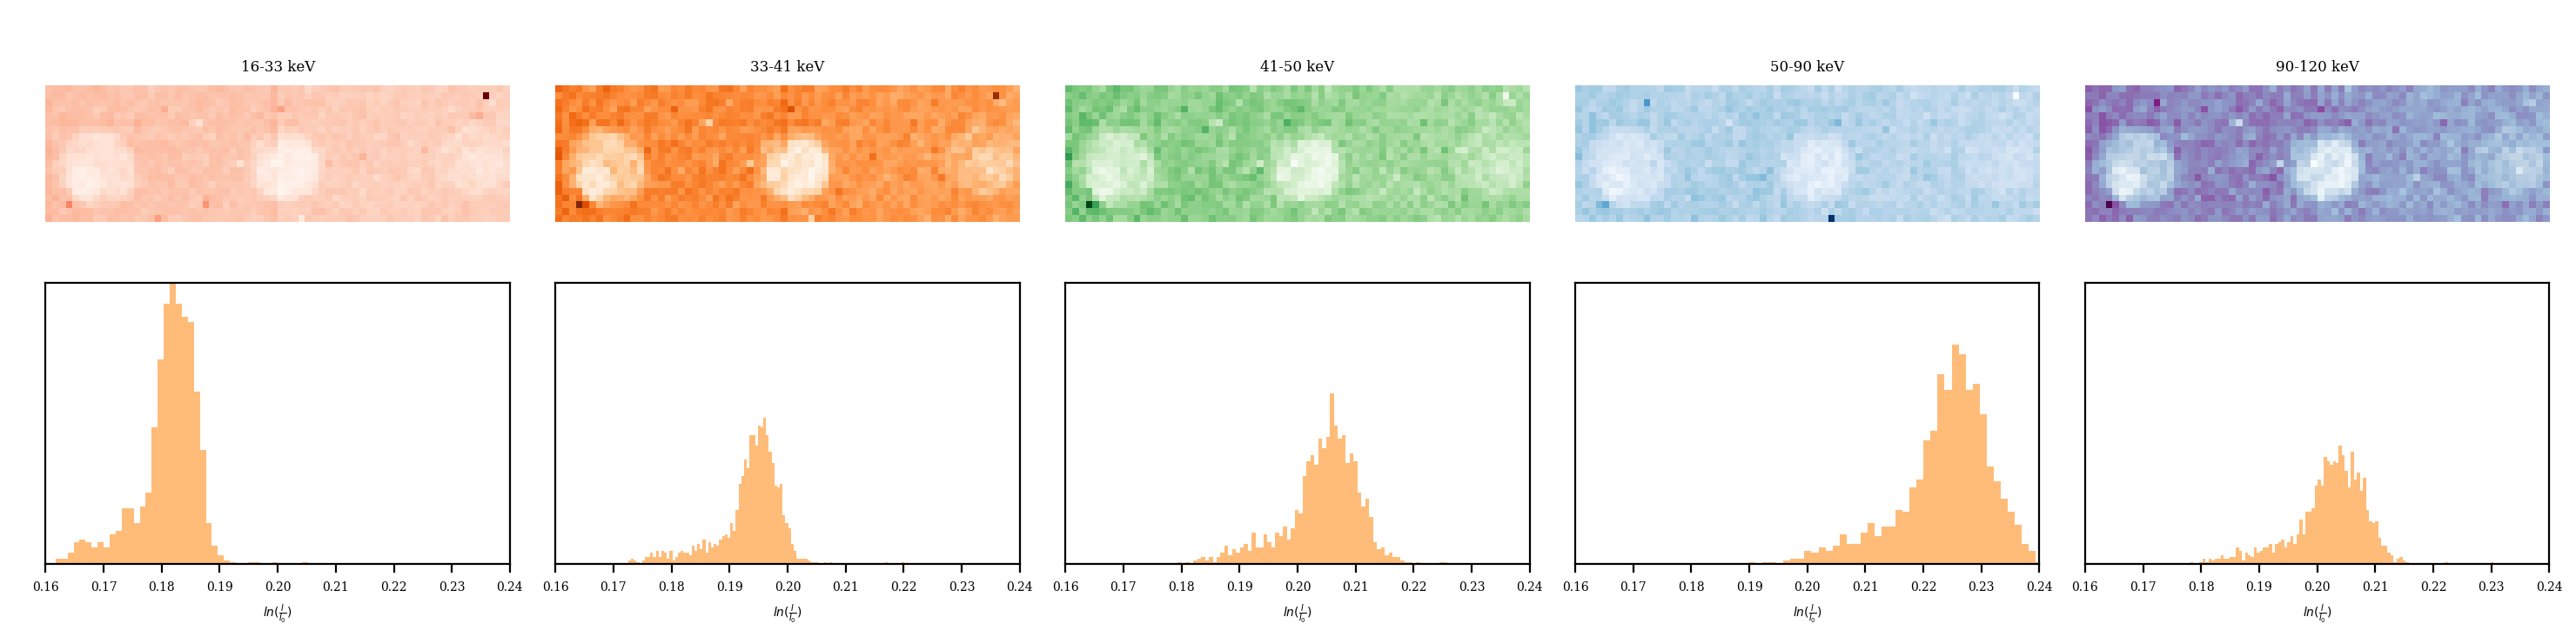
\includegraphics[width=\textwidth]{figures/poly_figure2.png}

\caption{The six channel images of PMMA embedded with poly-propylene are shown with different colormaps corresponding to their energy, red being lower energy while violet is higher energy. A histogram of the log intensity corresponding to each image is shown below the respective image.}
\label{demonstrating_bins}
\end{figure}

\subsubsection{Dimensional Reduction}

\begin{wrapfigure}{R}{0.5\textwidth}
  
  \begin{center}
    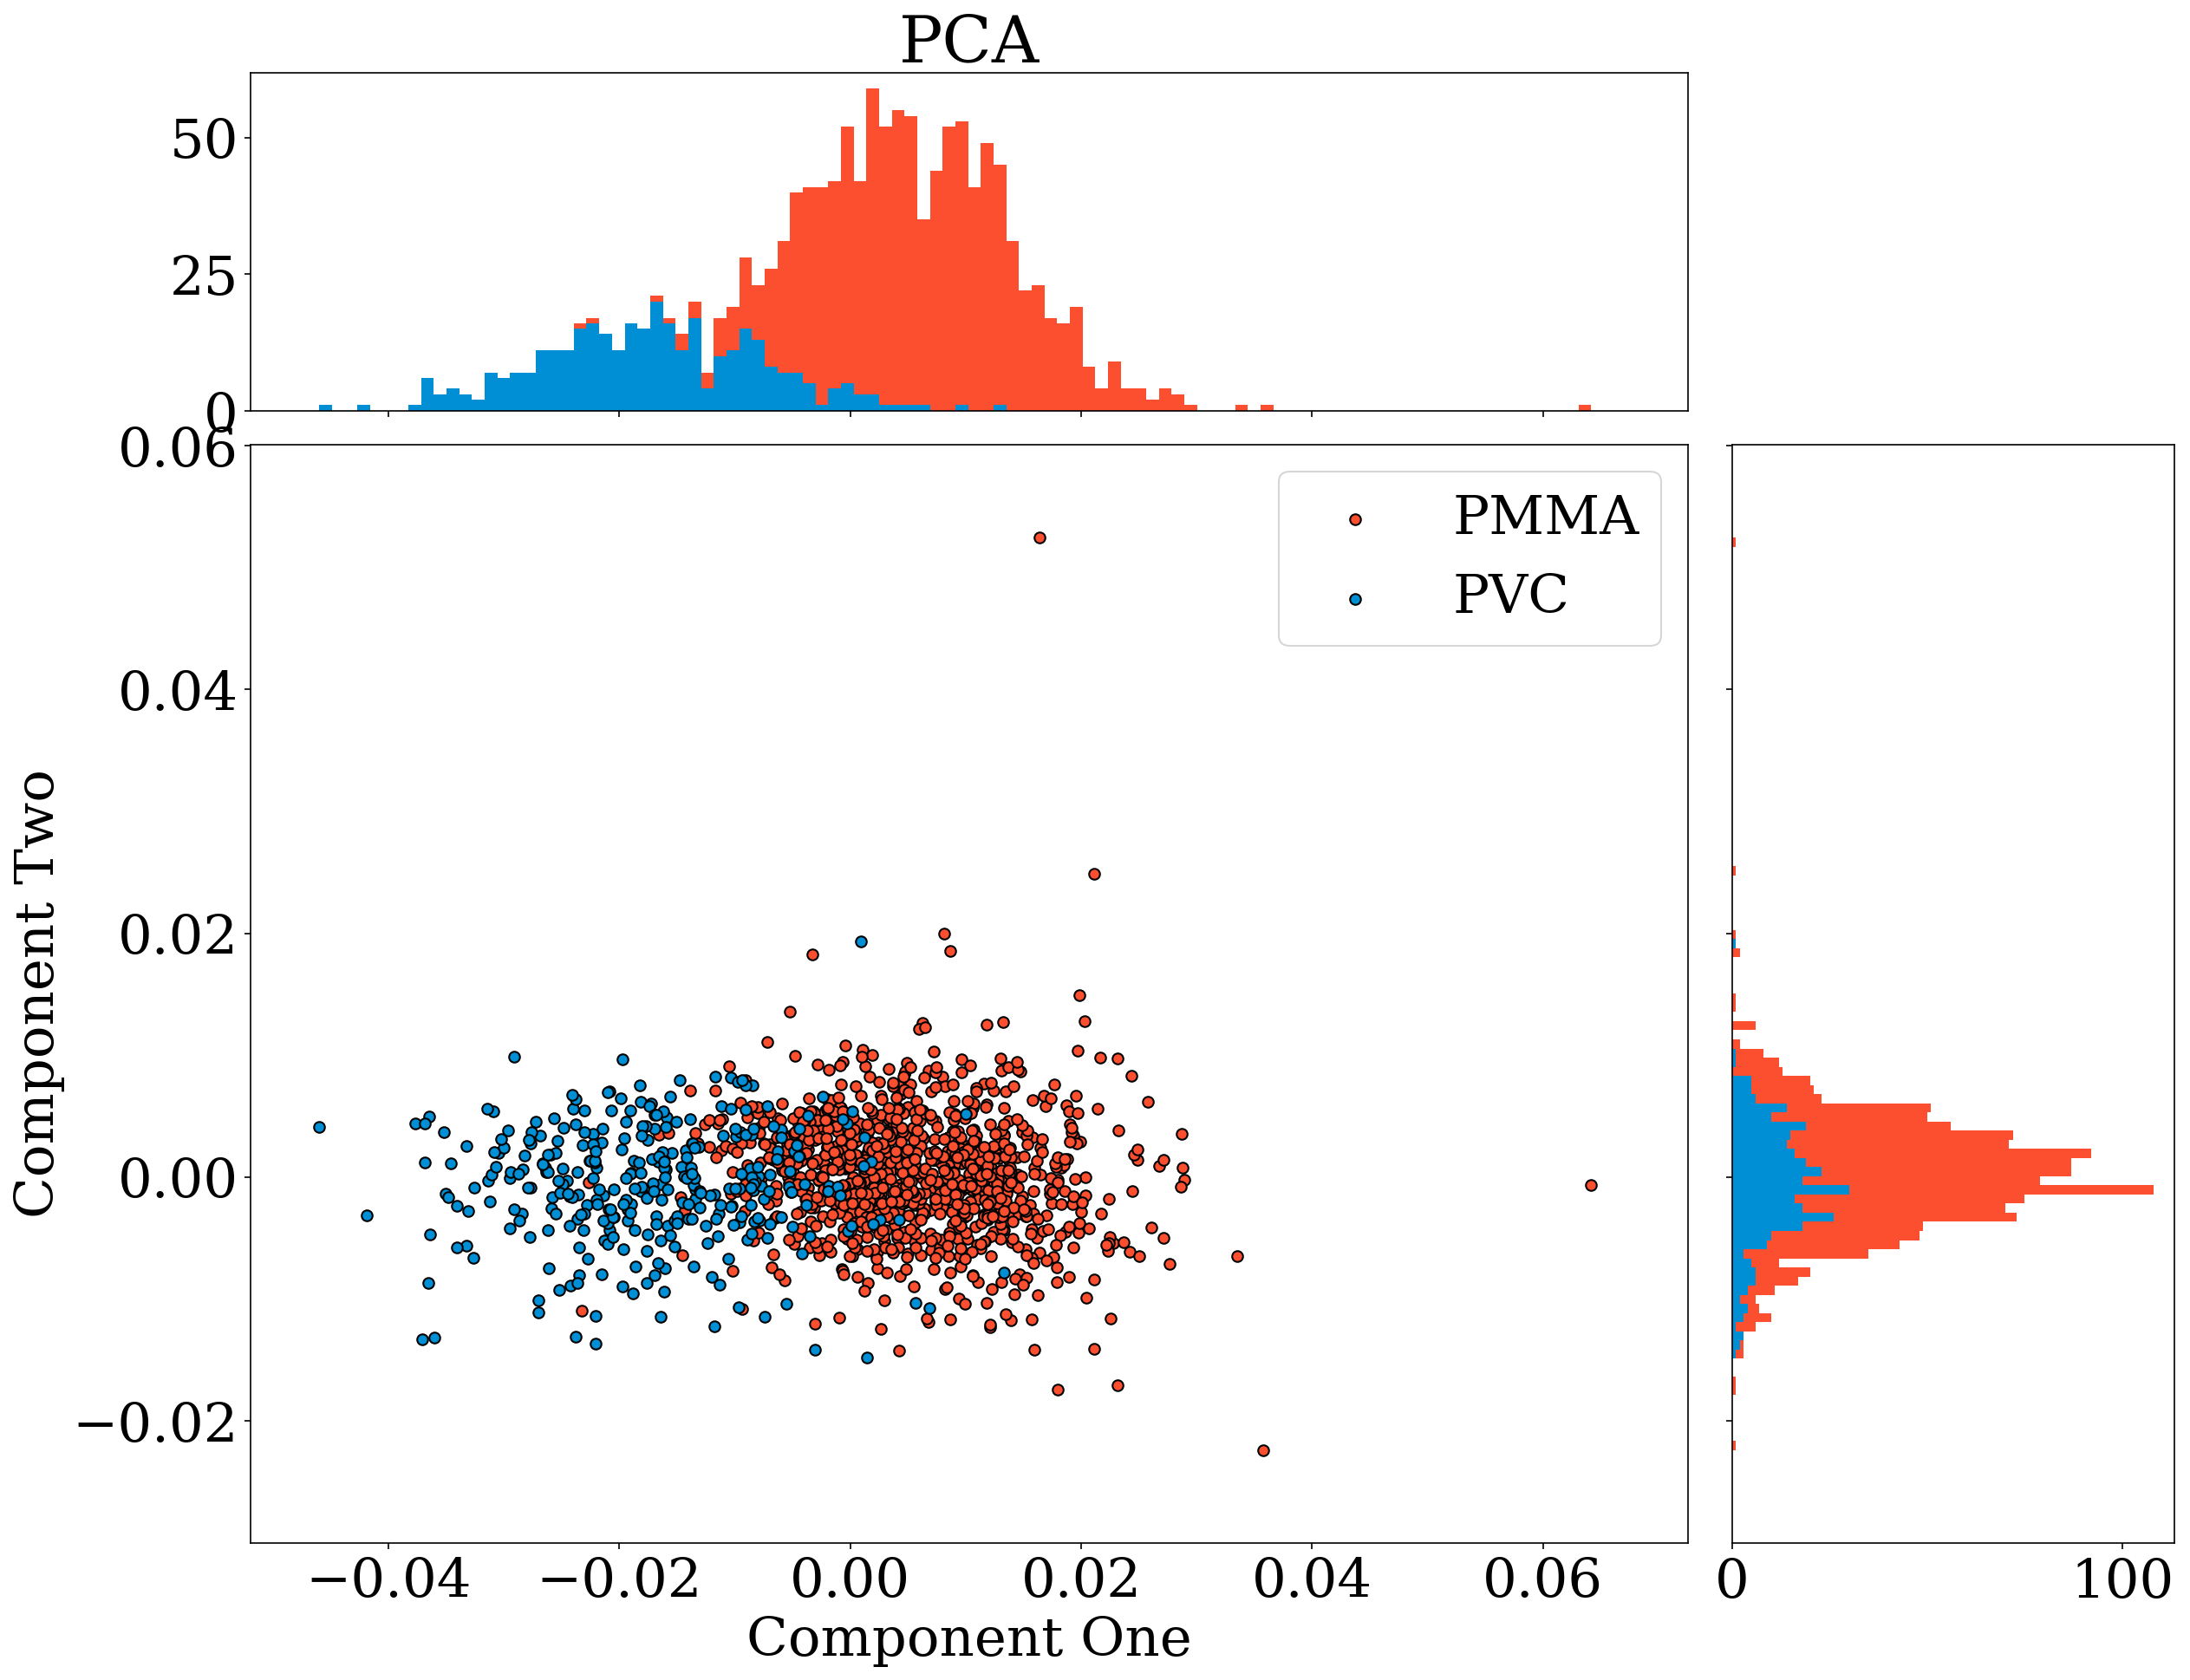
\includegraphics[width=0.48\textwidth]{figures/PCAnone.png}
  \end{center}
  
  \caption{The first two principle components of the data displayed as a scatter plot.}
  \label{PCA}
  
\end{wrapfigure}

Dimensional reduction methods were applied in this work to increase class separation and reduce noise in the data, methods were implemented in Python (Python Software Foundation) using sci-kit learn \cite{Pedregosa2011Scikit-learn:Python}. The three dimensional reduction thought suitable for this task were principle component analysis (PCA), independent component analysis (ICA), and non-negative matrix factorization (NMF). A visualization of the effect of reducing the data to two dimensions can be seen in Figures \ref{PCA},\ref{ICA}, and \ref{NMF}.

\subsubsection{Principal Component Analysis}

The first data reduction method employed in this study was Principle Component Analysis (PCA) \cite{Jolliffe2016PrincipalDevelopments.}. PCA decomposed the covariance matrix into eigenvalues and eigenvectors, sorting the eigenvectors in terms of the magnitude of their eigenvalue one finds the directions of highest variance in the data. The data is then projected into a lower dimensional orthogonal space defined by the eigenvectors with the most variance. This method results in a loss of information, however this loss of information is usually relatively small and ideally the discarded dimensions in the data amount to noise. PCA can be seen in Figure \ref{PCA}. PCA is fast, linear and sees application in many domains. 

\begin{wrapfigure}{R}{0.5\textwidth}
  
  \begin{center}
    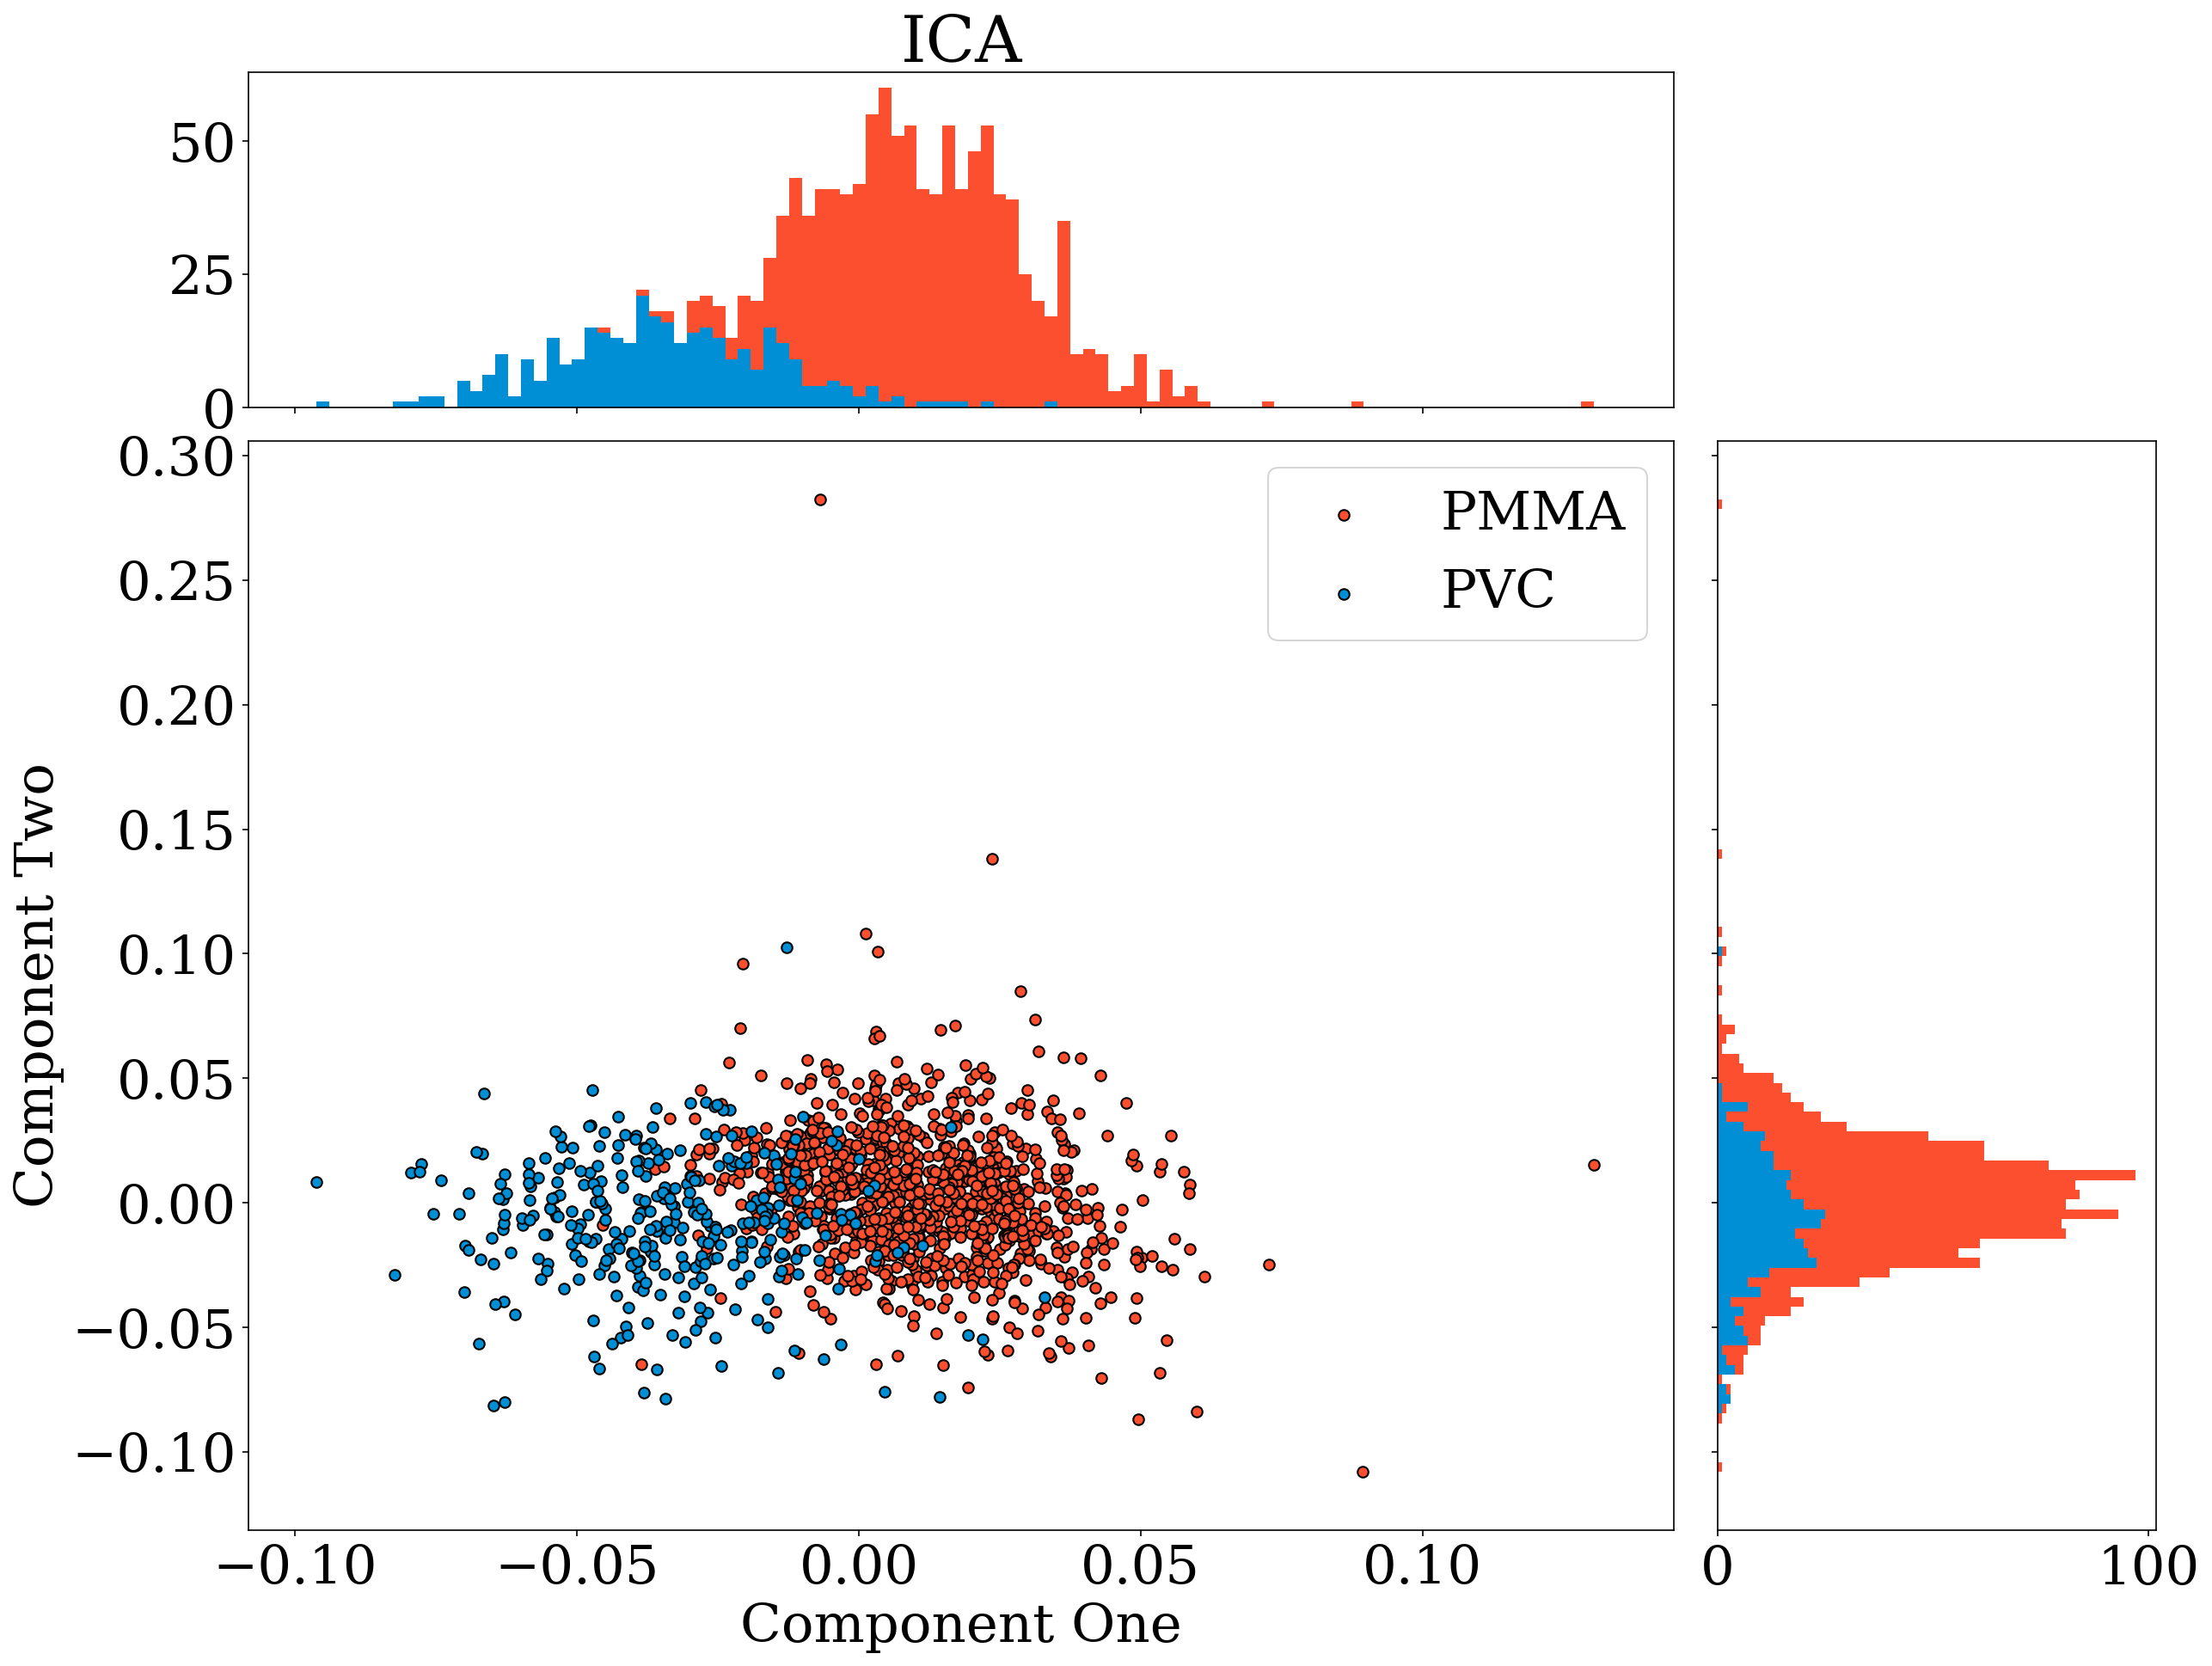
\includegraphics[width=0.48\textwidth]{figures/ICAnone.png}
  \end{center}
  
  \caption{The first two independent components of the data displayed as a scatter plot.}
  
  \label{ICA}
\end{wrapfigure}

\subsubsection{Independent Component Analysis}

Typically not used for dimension reduction but for blind source seperation, independant component analysis (ICA) is used for seperating a mixed signal into its constituent signals and is often used in audio analysis but has seen use in hyperspectral imaging \cite{Villa2009OnAnalysis}. Using ICA we frame the segmentation of the two images as a decomposition in which the image is a weighted addition of two signals. Idealy in our case these signals would be the background material (PMMA) and the contaminant. A demonstration of using ICA on PTFE embedded in PMMA can be seen in Figure \ref{ICA}. A more in depth explination of ICA can be found in appendix. The algorithm used for ICA in this work was the FastICA \cite{Hyvarinen2000IndependentApplications} algorithm implemented in scikit learn.

\begin{wrapfigure}{R}{0.48\textwidth}
  
  \begin{center}
    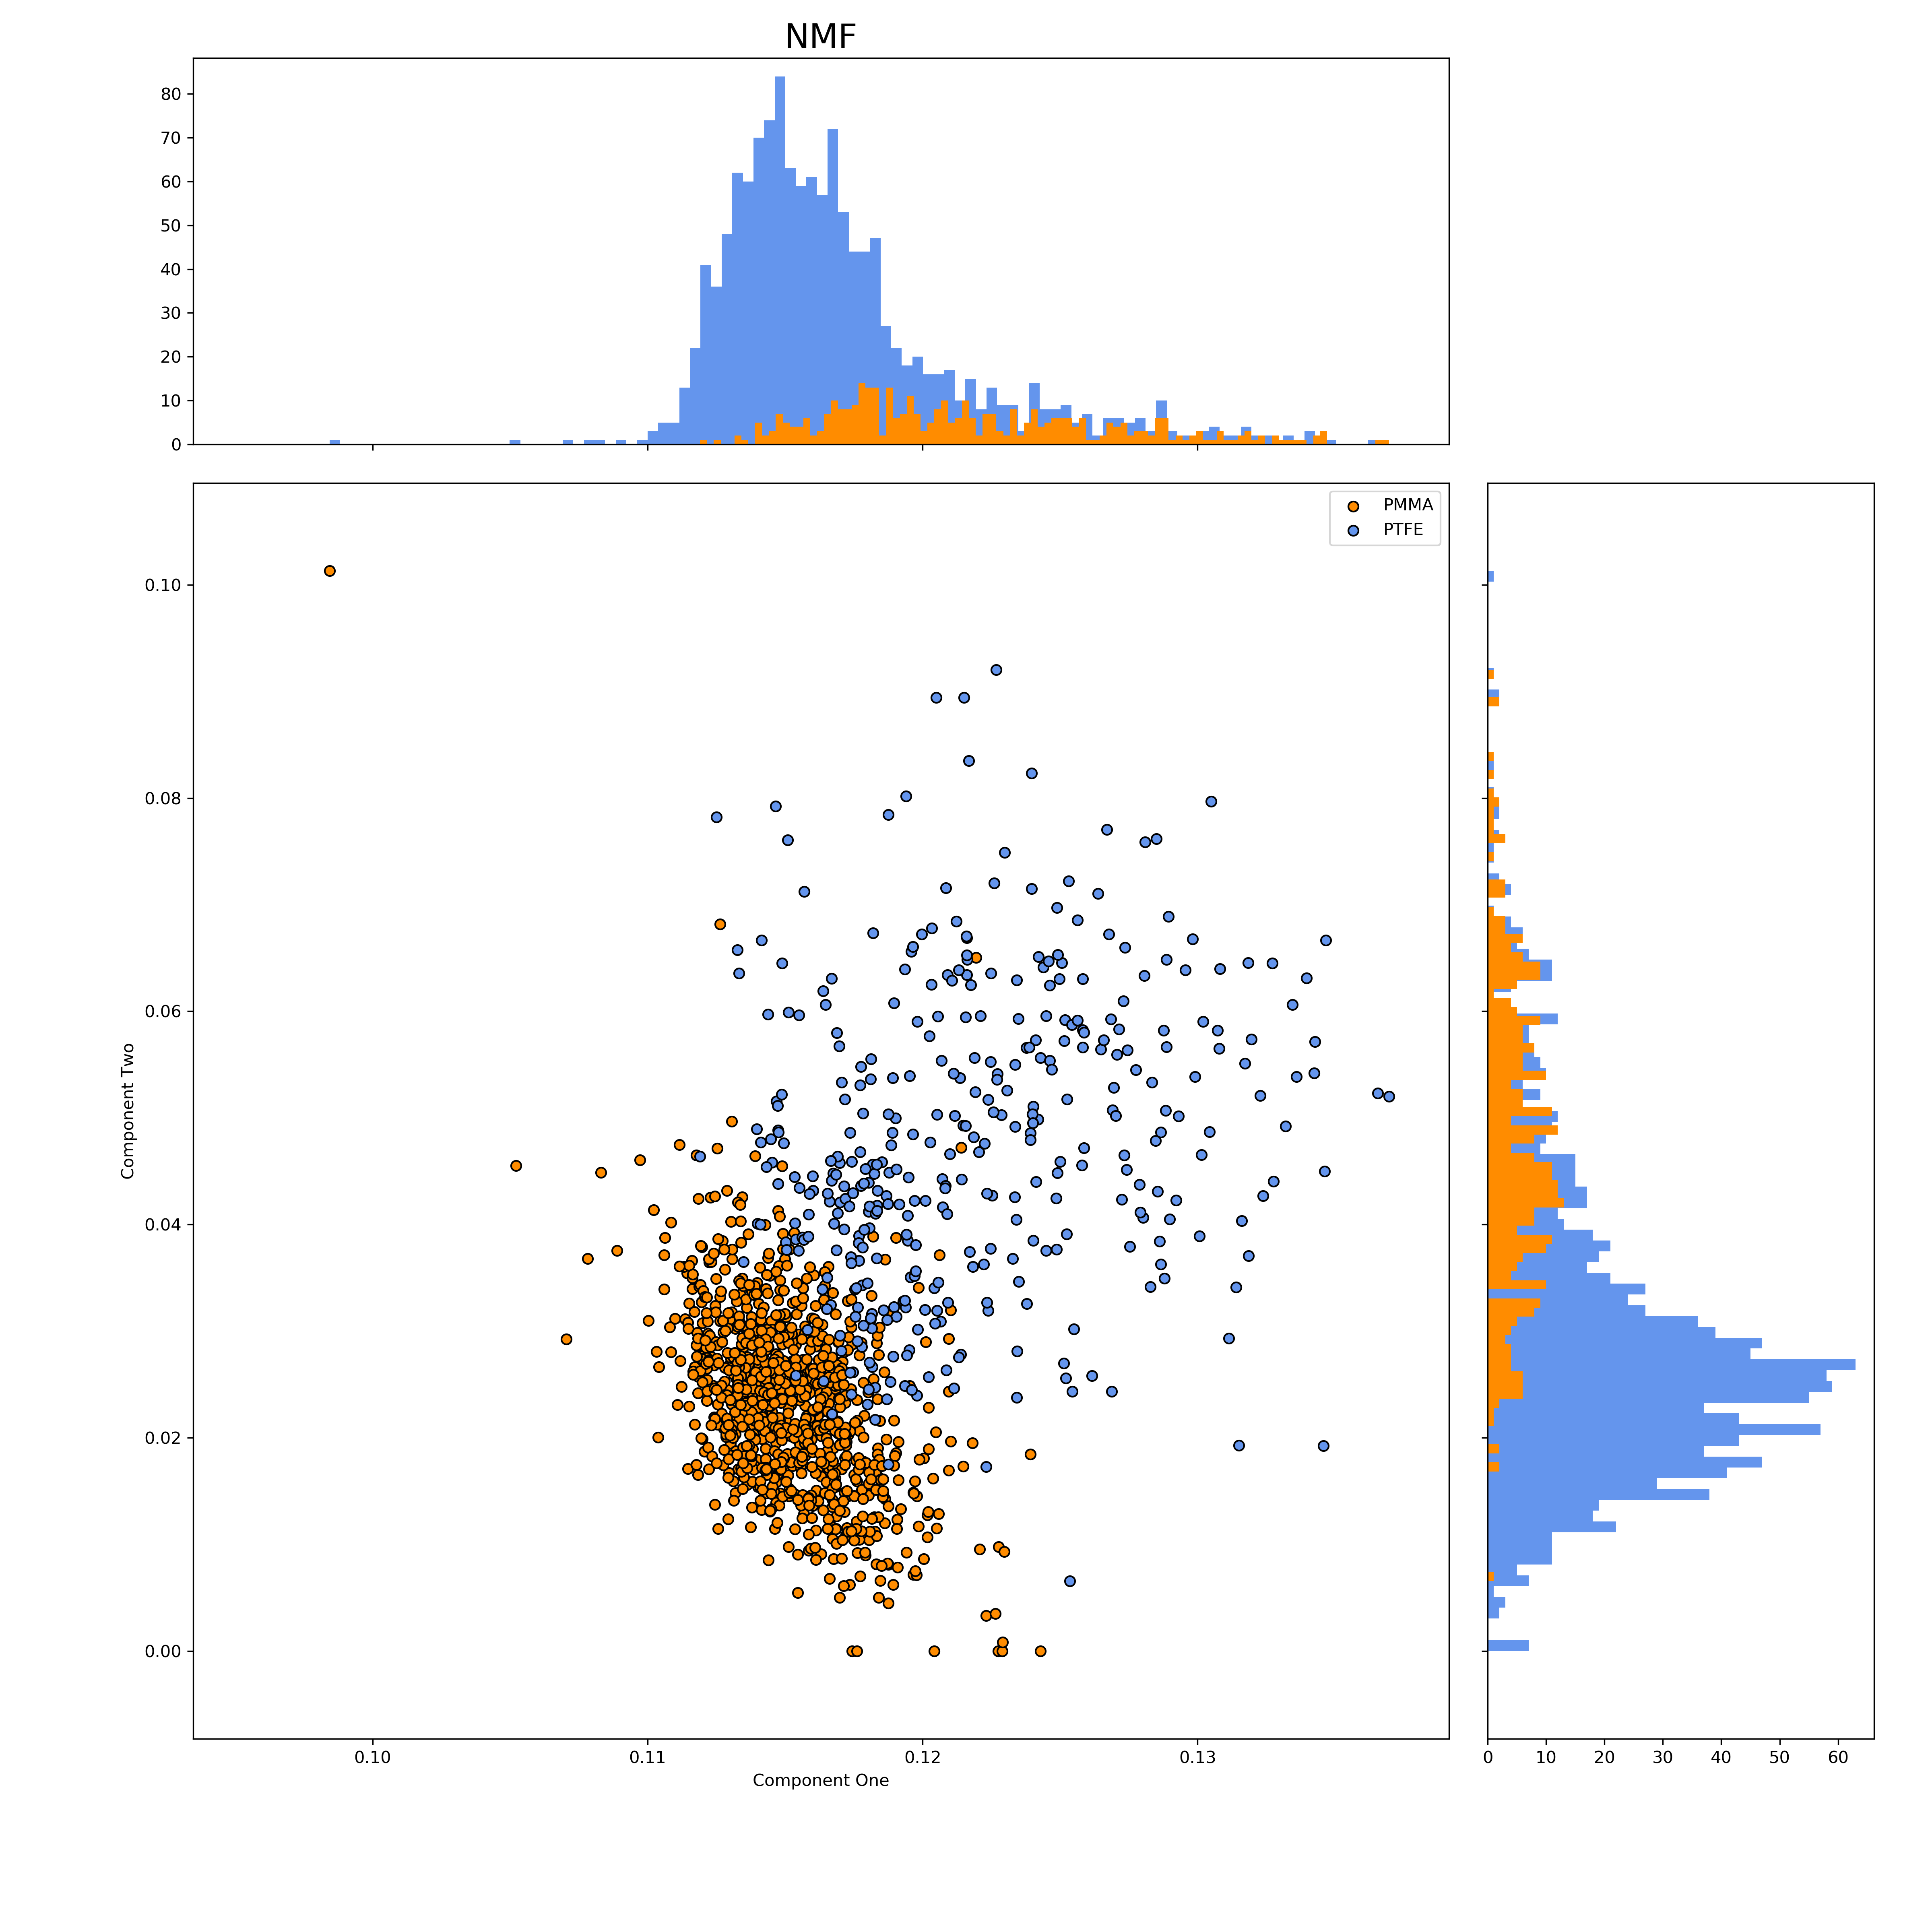
\includegraphics[width=0.48\textwidth]{figures/NMFnone.png}
  \end{center}
  
  \caption{The first two non-negative factorization components of the data displayed as a scatter plot.}
  
  \label{NMF}
\end{wrapfigure}

\subsubsection{Non-negative Matrix Factorization}

NMF assumes the Matrix $V$ is the product of the two matrices $W$ and $H$ such that : $V = WH$. 

When multiplying matrices the dimension of the factor matrices $W$ and $H$ may be much less that the product matrix. One can think of the two factor matrices as a feature matrix $W$ and a coefficient matrix $H$.

Thus, if one can find matrices $W$ and $H$ that have fewer dimensions than $V$, one can reconstruct the matrix $V$ in the lower dimensional space defined by $W$. To find the matrices $W$ and $H$ numerically we try to minimize the error defined by:

\begin{equation}
\min_{W,H} || V - WH ||_F, subject to W \geq 0, H \geq 0
\end{equation}

This was done in using scikit-learn's NMF function using gradient descent. A demonstration of NMF on PTFE embedded in PMMA can be seen in Figure \ref{NMF}.

\subsection{Clustering Methods}

\subsubsection{K-means}

The first clustering method implemented was k-means clustering. K-means was implemented using the k-means++ algorithm of \cite{ArthurK-means++:Seeding}. Different distance metrics were used, however none of the distance metrics tried improved performance over the squared euclidean distance, thus squared euclidean distance was used. K-means is a general purpose, fast and scalable clustering algorithm. Like many of the methods examined K-means requires the parameter $K$ which descibes the number of clusters in the data. This parameter can be hard to estimate in some cases. Methods for defining the parameter $K$ will be seen in the following metrics section.

\begin{figure}[t!]
    \centering
    \begin{subfigure}[b]{0.48\textwidth}
        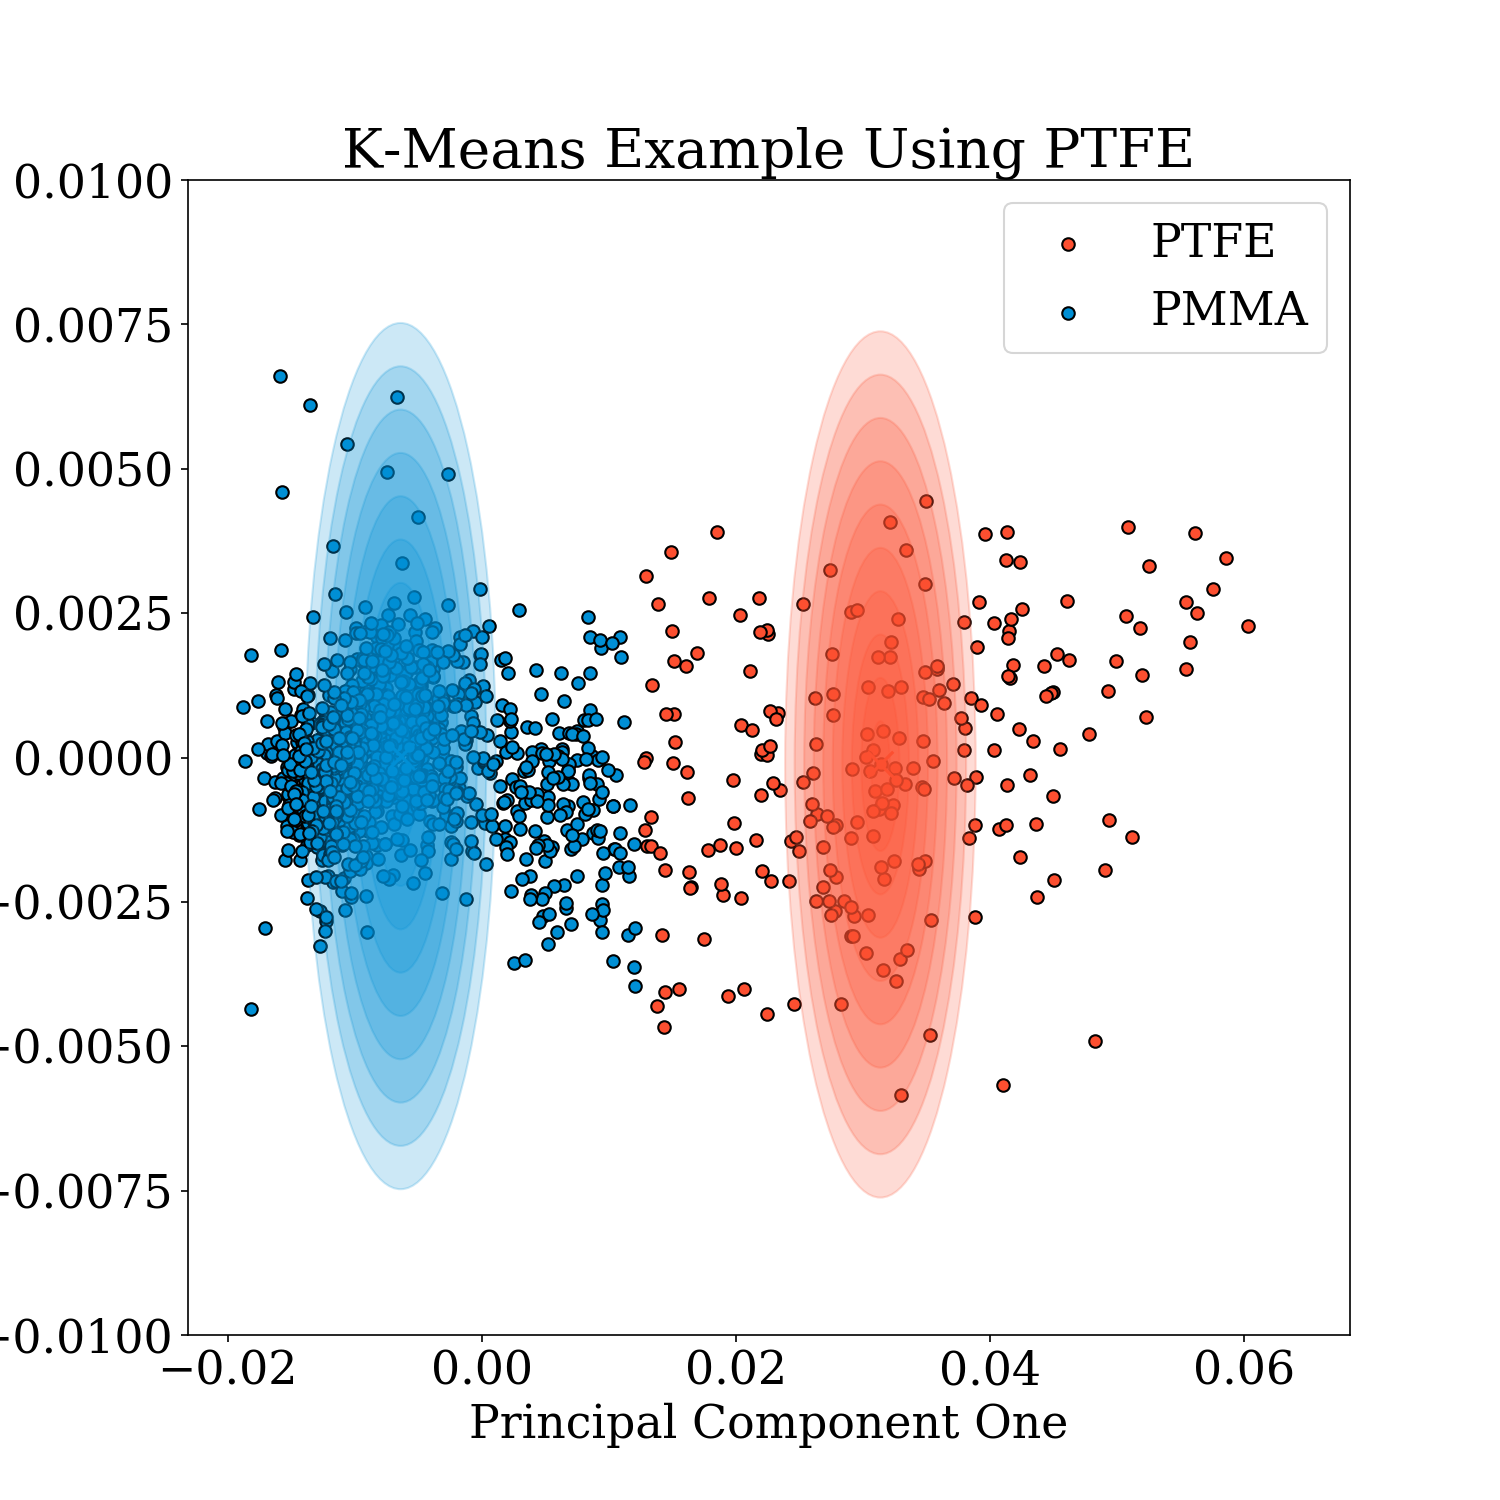
\includegraphics[width=\textwidth]{figures/Kmeans.png}
    \end{subfigure}
    ~ %add desired spacing between images, e. g. ~, \quad, \qquad, \hfill etc. 
      %(or a blank line to force the subfigure onto a new line)
    \begin{subfigure}[b]{0.48\textwidth}
        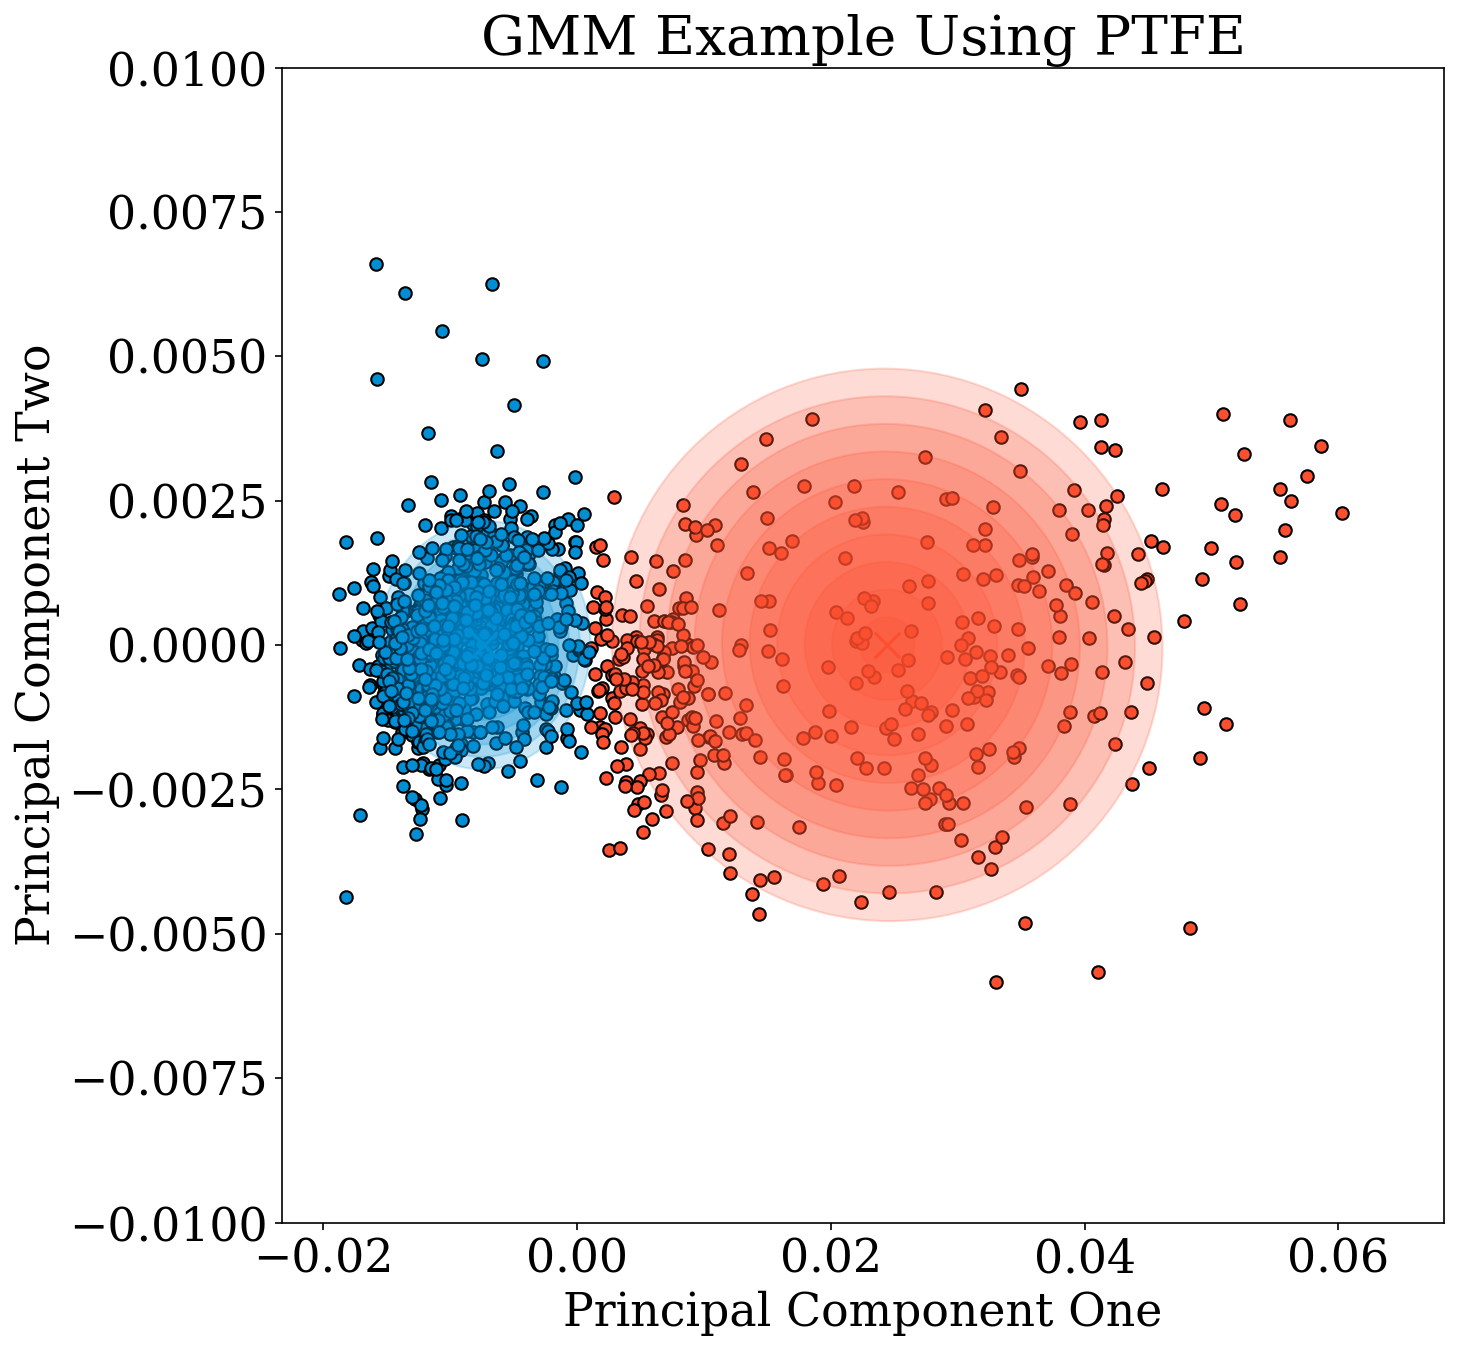
\includegraphics[width=\textwidth]{figures/GMM.png}
    \end{subfigure}

    \caption{Clustering Methods}\label{clustering_methods}
\end{figure}

\subsubsection{Gaussian Mixture Models}

A gaussian mixture model (GMM) can be used as a clustering method that implicitly accounts for the Gaussian nature of a dataset. This can be useful in many applications where the data is sum of many random variables. In X-ray we see Poisson distributions which can be approximated by Gaussians. First we will discuss a general mixture model and then we will see how it is changed by assuming a Gaussian distribution. A more complete overview of GMMs can be found at \cite{DinovExpectationTutorial}.

General mixture models contain $N$ data points, each assumed to be a mixture of $K$ components, with all of these components assumed to be from the same family of distributions. In this case a Gaussian distribution. However these distributions are allowed to have different parameters, in this case different means and variances. The model also includes the identity of the mixture component to which each data point belongs. Also necessary is a weighting of each of the $K$ components and sets of parameters for each of the distributions, in this case means and variances for the Gaussians.

In this study the number of components used was two and a further constraint was put on the variance of the GMMs to assure that they are spherical in the PCA case. This constraint will be discussed in more depth in the results and discussion section.

\subsubsection{Other Clustering Methods}

A number of other clustering methods were compared. These additional methods and their parameters are summarized in table \ref{tab1}.


% Please add the following required packages to your document preamble:
% \usepackage[table,xcdraw]{xcolor}
% If you use beamer only pass "xcolor=table" option, i.e. \documentclass[xcolor=table]{beamer}
\begin{table}[htbp]
\begin{tabular}{|l|l|l|l|}
\hline

Method name                                                            & Parameters                                                                                                                                         & Notes on Parameters                                                                                                                & Geometry (metric used)                                                      \\ \hline
K-Means                                                                & number of clusters                                                                                                                                 & \begin{tabular}[c]{@{}l@{}}1 or 2,\\ defined by silhouette\\ score\cite{Rousseeuw1987Silhouettes:Analysis}\end{tabular}                                                    & \begin{tabular}[c]{@{}l@{}}Squared Euclidean\\ Distance\end{tabular}        \\ \hline
Mean-shift \cite{Fukunaga1975TheRecognition}                                                             & bandwidth                                                                                                                                          & \begin{tabular}[c]{@{}l@{}}estimated using\\ scikit-learn's bandwidth\\ estimator\end{tabular}                                     & \begin{tabular}[c]{@{}l@{}}Euclidean \\ Distance\end{tabular}               \\ \hline
Spectral clustering                                                  & \begin{tabular}[c]{@{}l@{}}number of clusters,\\ eigensolver,\\ label assignment\end{tabular}                                                      & \begin{tabular}[c]{@{}l@{}}1 or 2,\\ ARPACK \cite{Lehoucq1998ARPACKMethods},\\ K-means\end{tabular}                                        & \begin{tabular}[c]{@{}l@{}}Nearest-neighbor \\ graph distance\end{tabular}  \\ \hline
\begin{tabular}[c]{@{}l@{}}Ward hierarchical\\ clustering \cite{Ward1963HierarchicalFunction}\end{tabular} & \begin{tabular}[c]{@{}l@{}}number of clusters,\\ connectivity matrix\end{tabular}                                                                  & \begin{tabular}[c]{@{}l@{}}1 or 2,\\ estimated as:\\ $1/2*(C+C')$\\ where C is the\\ K neighbors graph of\\ the data.\end{tabular} & \begin{tabular}[c]{@{}l@{}}Squared\\ euclidean\\ distance\end{tabular}      \\ \hline
HDBSCAN \cite{Campello2015HierarchicalDetection}                                                                & \begin{tabular}[c]{@{}l@{}}minimum samples,\\ minimum cluster size,\\ metric\end{tabular}                                                          & \begin{tabular}[c]{@{}l@{}}10,\\ 10,\\ minkowski\end{tabular}                                                                      & \begin{tabular}[c]{@{}l@{}}Distances between\\ nearest points\end{tabular}  \\ \hline
Gaussian Mixture                                                       & \begin{tabular}[c]{@{}l@{}}number of clusters,\\ covariance type\end{tabular}                                                                      & \begin{tabular}[c]{@{}l@{}}1 or 2,\\ spherical\end{tabular}                                                                        & \begin{tabular}[c]{@{}l@{}}Mahalanobis \\ distances to centers\end{tabular} \\ \hline
Birh \cite{Zhang1996BIRCH}                                               & \begin{tabular}[c]{@{}l@{}}number of clusters,\\ branching factor, \\ threshold\end{tabular}                                                       & \begin{tabular}[c]{@{}l@{}}1 or 2,\\ 19,\\ 0.0001\end{tabular}                                                                     & \begin{tabular}[c]{@{}l@{}}Euclidean \\ distance\end{tabular}               \\ \hline
Gaussian Mixture                                                       & \begin{tabular}[c]{@{}l@{}}number of clusters,\\ covariance type,\\ weight concentration\\ prior type,\\ weight concentration\\ prior\end{tabular} & \begin{tabular}[c]{@{}l@{}}1 or 2,\\ spherical,\\ dirichlet process,\\ \\ 1/(number of clusters)\end{tabular}                      & \begin{tabular}[c]{@{}l@{}}Mahalanobis \\ distances to centers\end{tabular} \\ \hline
\end{tabular}
\label{tab1}
\end{table}

\subsection{Metrics}
\subsubsection{V-measure}

To evaluate the effectiveness of the clustering methods a ground truth was acquired for each radiograph. These ground truths were manually segmented with the help of a reference photograph of the material imaged. For clarity, the labels we give to the ground truth will be referred to as classes while the results of the clustering methods will be clusters.

Evaluation compared these ground truth classes to clusters. When comparing the clusters to the ground truth two metrics were considered: The first metric is homogeneity. Homogeneity is satisfied if a cluster contains data points of a single class. We note, if using homogeneity as the sole evaluation metric, assigning all points to one class would attain a perfect evaluation score. Thus we introduce a second evaluation metric, completeness, satisfied if all data points of a single class are in a single cluster. 

Formulating these metrics mathematically using the method described by Rosenberg and Hirschberg \cite{Rosenberg2007V-Measure:Measure} using combination of both homogeneity $h$ and completeness $c$. This combination is called the V-measure and is the harmonic mean of homogeneity and completeness.

\begin{equation}
v = 2 \cdot \frac{h \cdot c}{h + c}
\end{equation}

With values ranging from assigning each point to a cluster at 0 to perfect clustering at 1. A mathematical treatment of V-measure is found in the appendix.

\subsubsection{Akaike Information Criterion}

The Akaike information criterion (AIC) \cite{Akaike1998InformationPrinciple} is an estimator of the relative quality of a statistical model for a given data set. Unlike a V-measure, AIC could not compare different clustering methods as most clustering models discussed don't include statistical models.

AIC is a function of the goodness of fit of a statistical model combined with a penalty for overfitting. In this work AIC tested the goodness of fit of the GMM's Gaussian, with a penalty proportional to the number of clusters. Used this way, AIC determines the optimal number of clusters.

Specifically the maximum likelihood found by the GMMs EM algorithm, $\hat L$, and the number of parameters $k$ were used as:

\begin{equation}
    AIC \, = \, 2k - 2\ln(\hat L)
\end{equation}

For a given model the lowest AIC denotes the best fit. More specifically an "elbow" or change in curvature of the AIC as a function of the number of components denotes the optimal number of components.

\subsubsection{Interpolating Bayesian Gaussian Mixture Model}

%Initial clustering results contained many pixels misclassified due to poor detector response, noise in the data and partial volume effects. To combat these effects a
Additional to the previous methods, a new method was also proposed the workflow is seen in Figure \ref{iterative_method}: A GMM was first trained on the data as described above. Within each cluster the distance from all the points to the center was calculated. Points greater than \%90 of the maximum were then identified as potential outliers. Each potential outlier was then interpolated spacialy using biharmonic interpolation \cite{Damelin2017OnAspects}. The GMM was then retrained using starting point defined by the end state of the previous iteration. The process was then repeated. The AIC of the model was monitored and the process was stopped when the AIC started to increase. In practice this amounted to between five and ten iterations. A result of this method can be seen in Figure \ref{iterative_method}.

\begin{figure}[htbp]
    \centering
    \begin{subfigure}[b]{0.32\textwidth}
        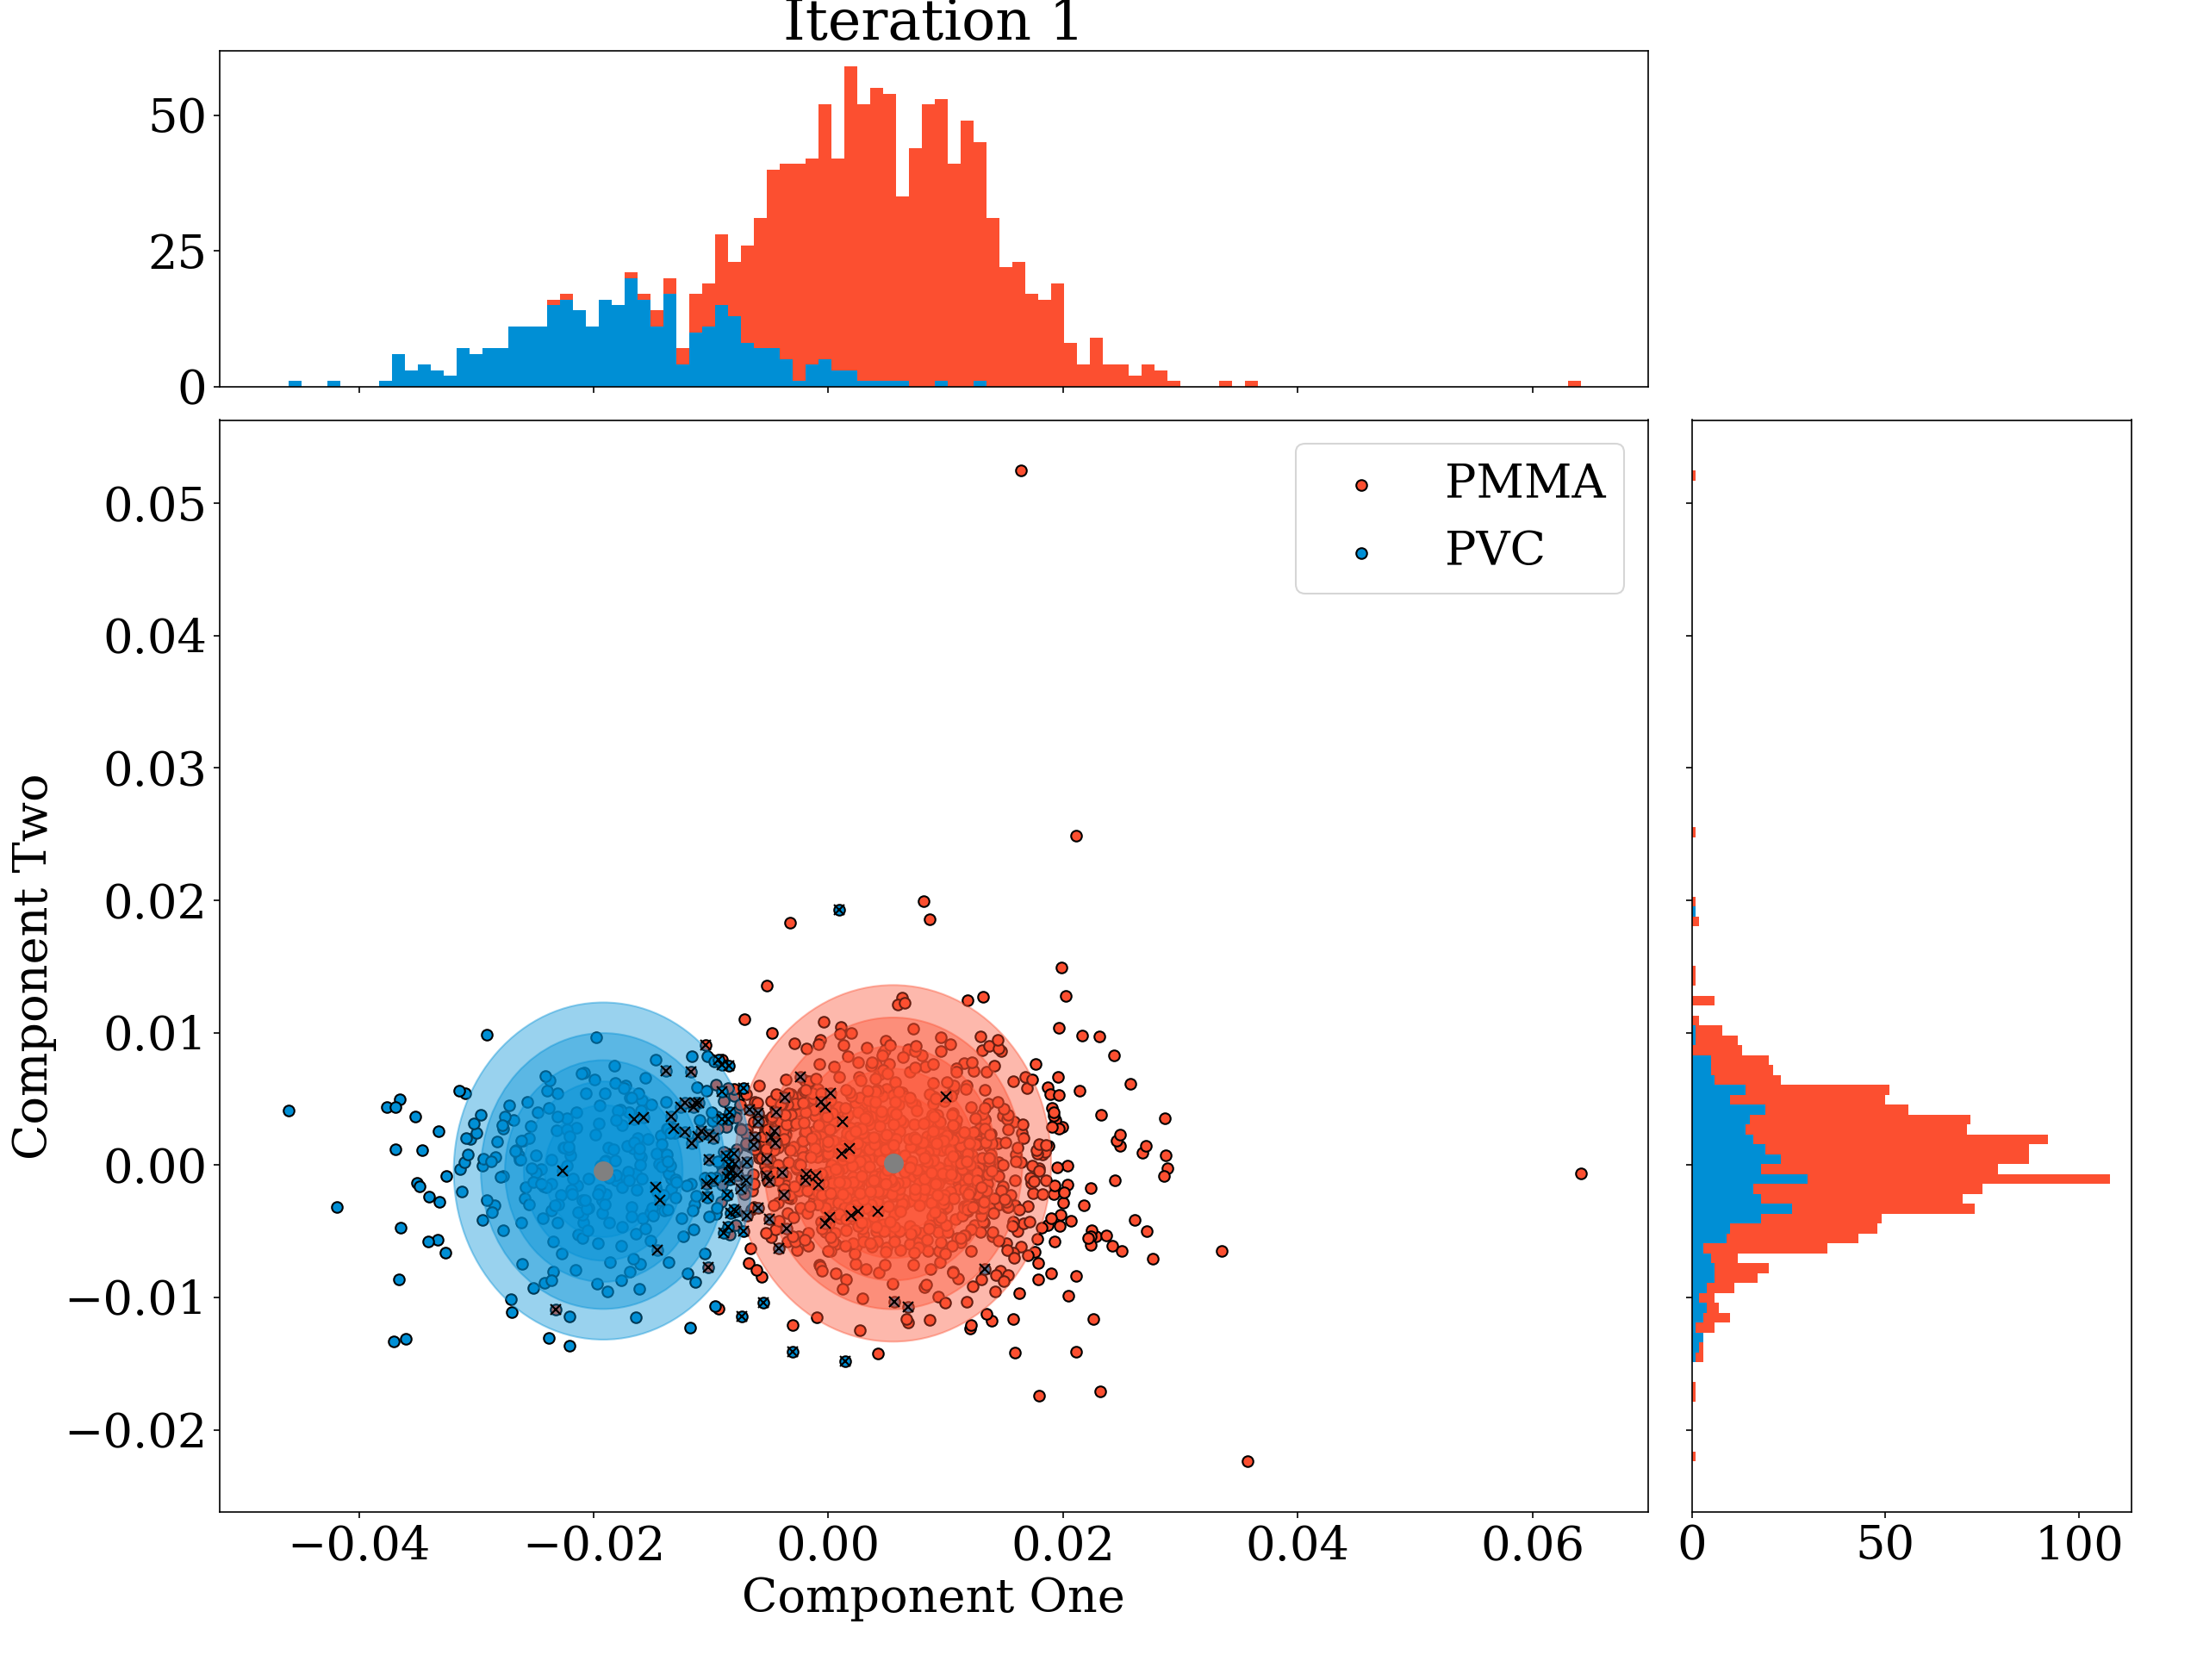
\includegraphics[width=\textwidth]{figures/PCAsphericalbefore.png}
    \end{subfigure}
    ~ %add desired spacing between images, e. g. ~, \quad, \qquad, \hfill etc. 
      %(or a blank line to force the subfigure onto a new line)
    \begin{subfigure}[b]{0.32\textwidth}
        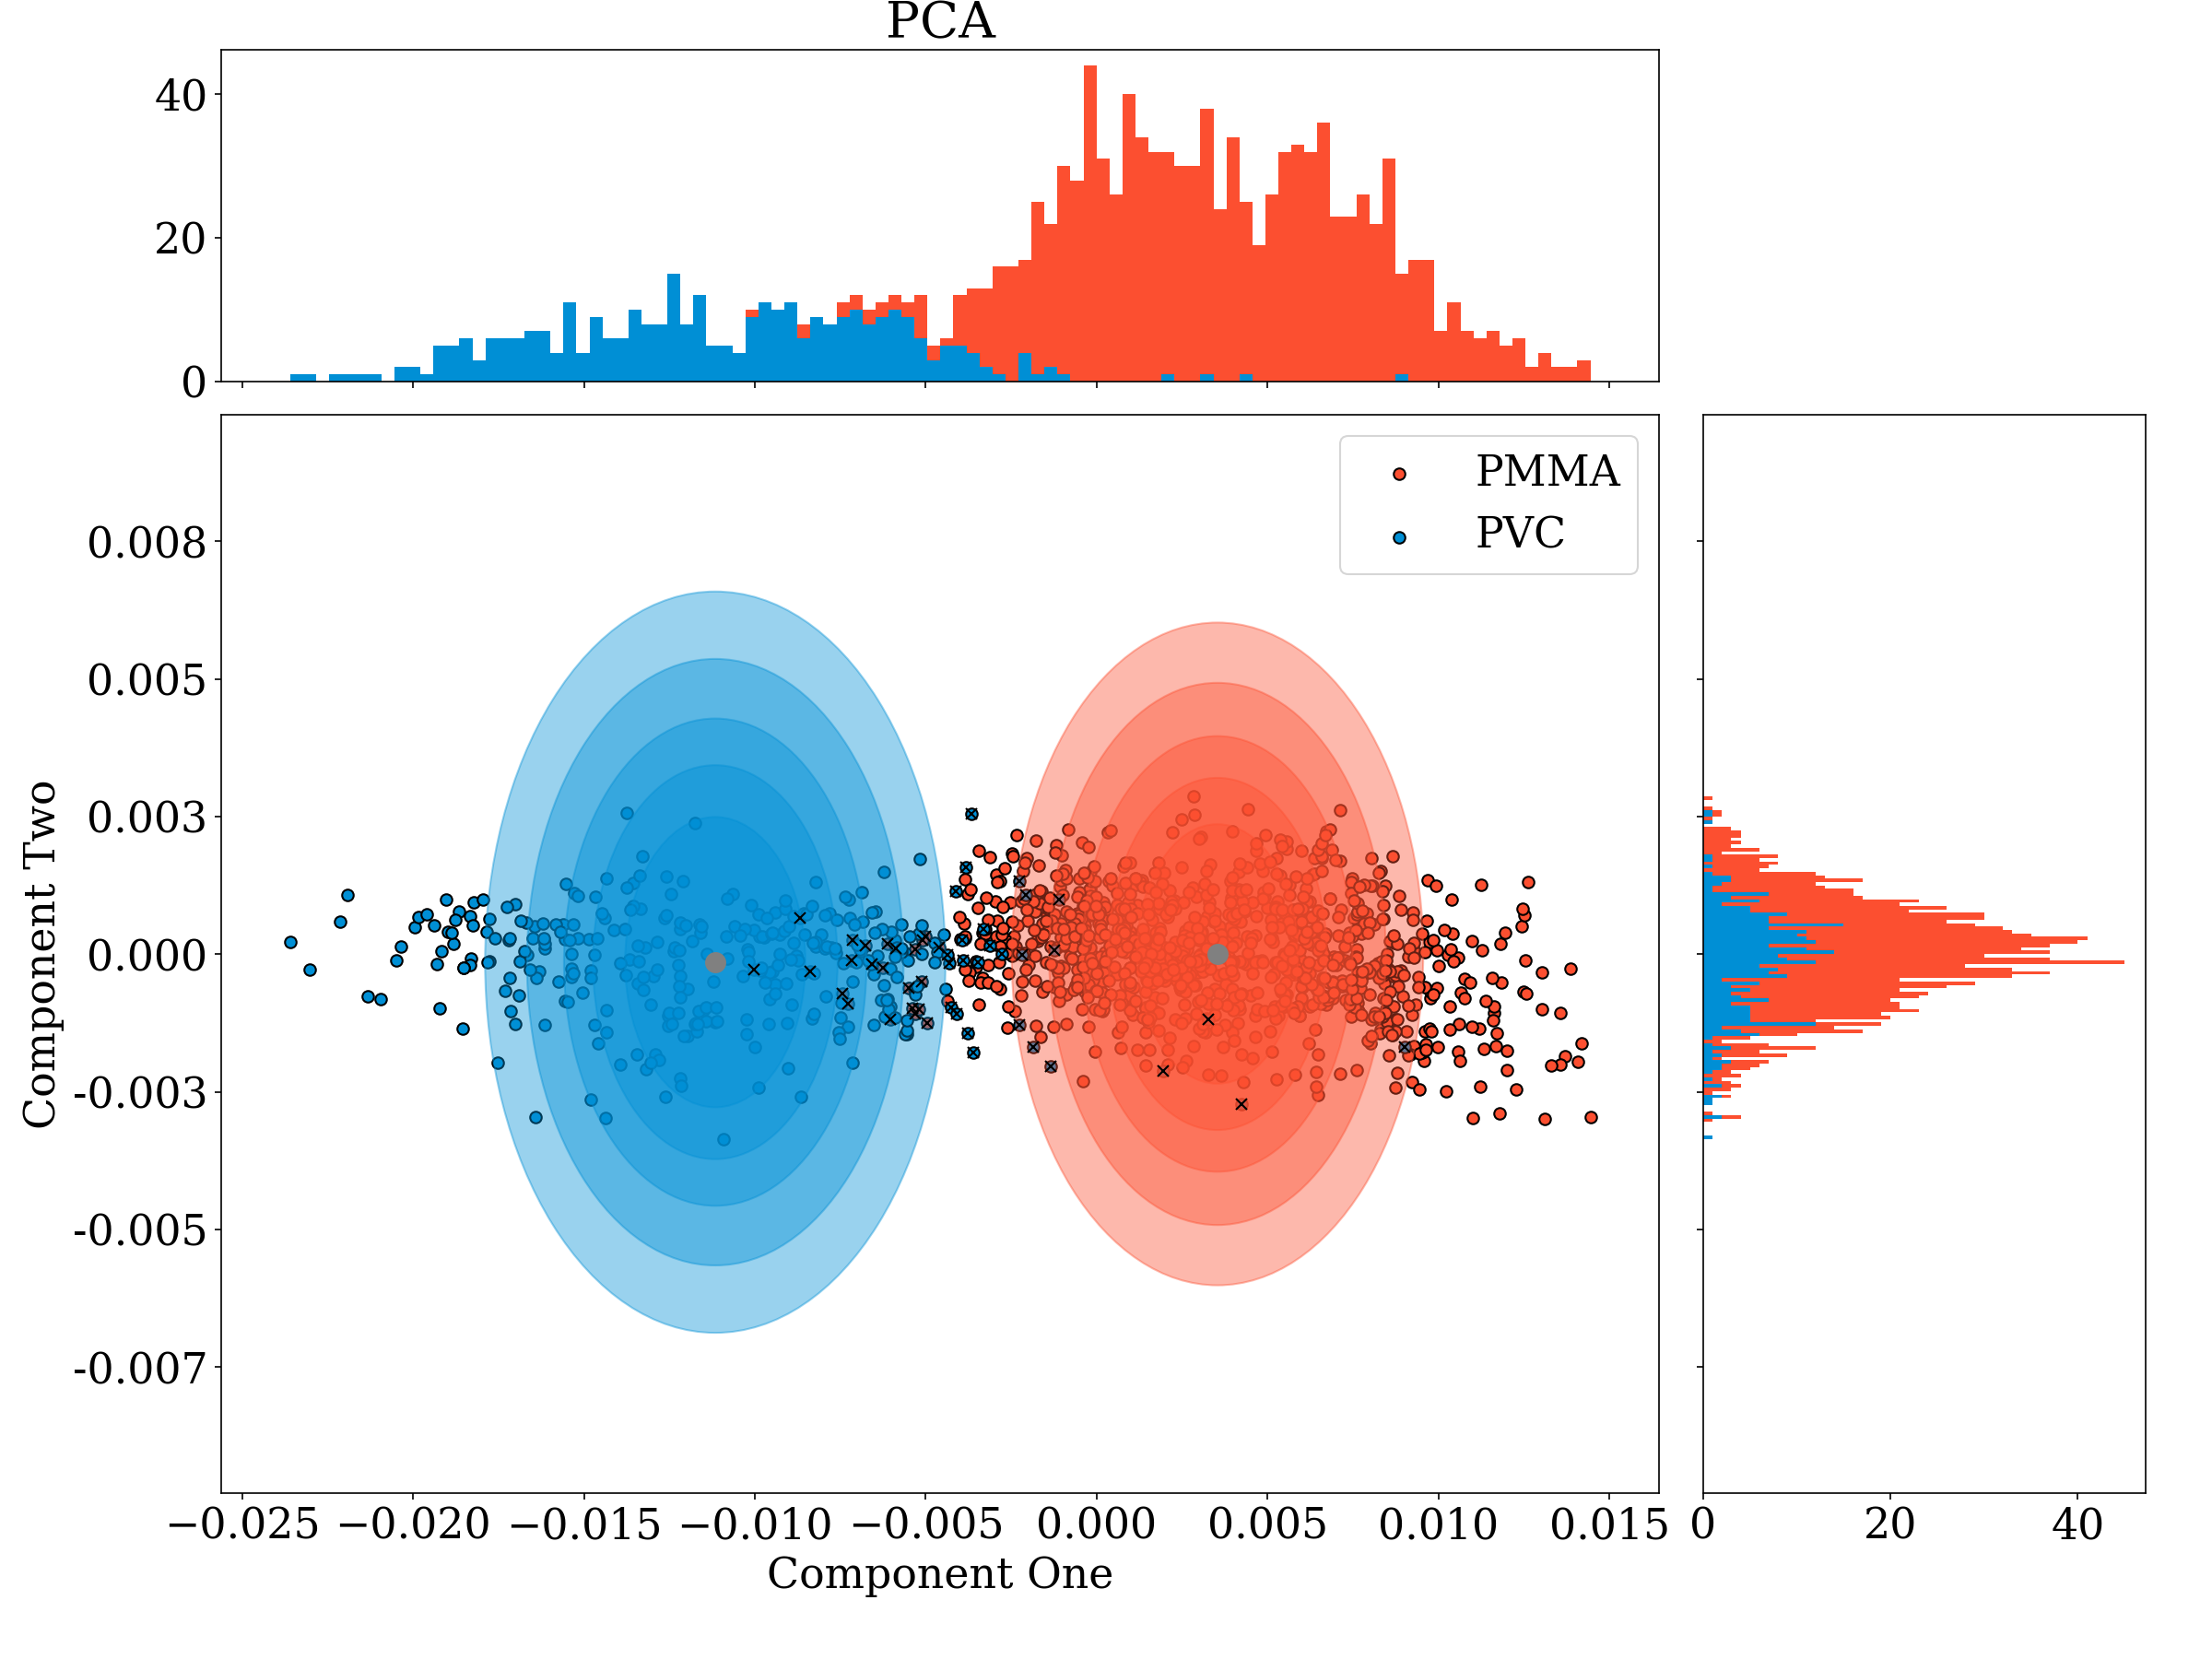
\includegraphics[width=\textwidth]{figures/PCAsphericalafter.png}
    \end{subfigure}
    \begin{subfigure}[b]{0.32\textwidth}
        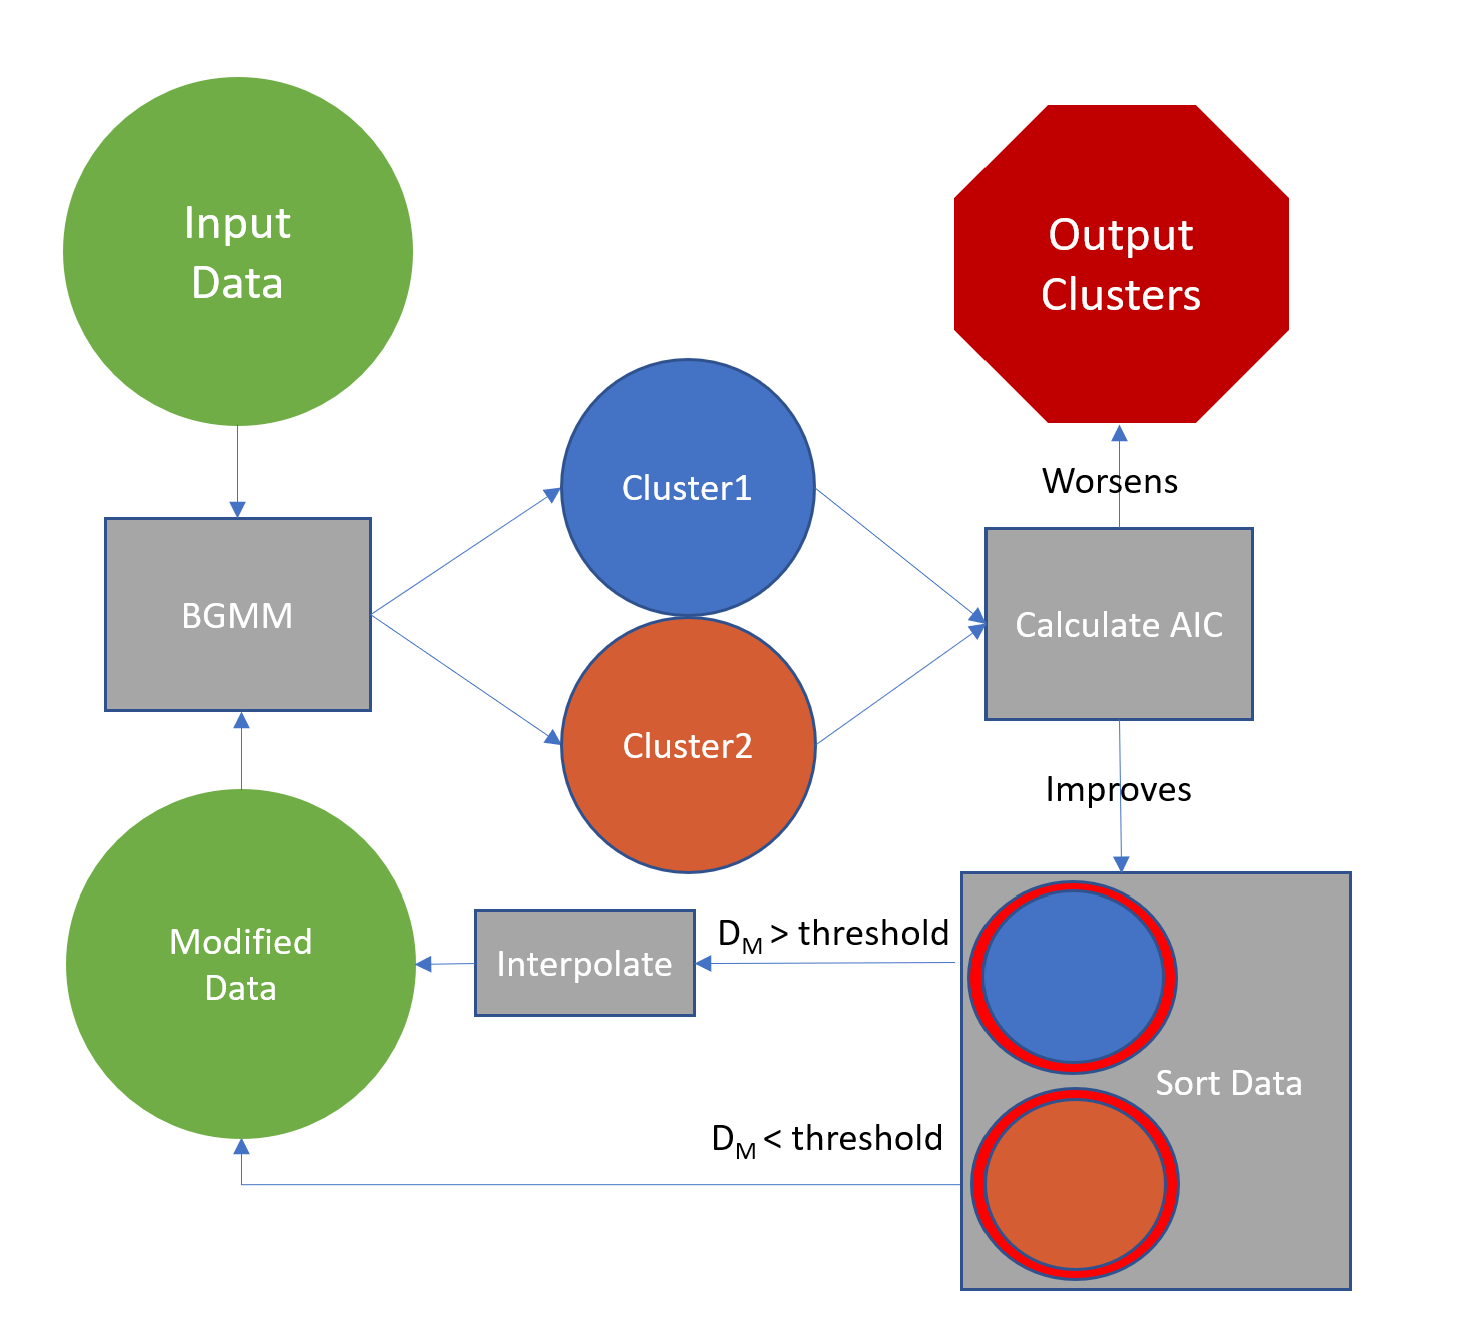
\includegraphics[width=\textwidth]{figures/algo_flow.png}
    \end{subfigure}
    \caption{Clustering Methods}
    \label{iterative_method}
\end{figure}

\subsubsection{Post-processing}

The aim of this work is to entirely automate image segmentation. Thus on top of the clustering it is necessary to introduce an identification layer. This layer will take the segmented image after the clustering and identify if there are two materials present or one. To do this the following framework was developed:

First a uniform filter is applied to the image so that the binary data becomes continuous. This acts to reduce the score of single pixels that have been identified. Secondly, we apply a threshold to the image that is slightly greater than zero in this case 0.2. Next, we fill all of the binary holes in the image to make candidates for segmentation more uniform. A bounding box is then created around all of the nonzero elements of the image and overlaid on the image as the final output.

%--------------------------------------------------------------------------------%
%%%%%%%%%%%%%%%%%%%%%%%%%%%%%% Results %%%%%%%%%%%%%%%%%%%%%%%%%%%%%%%%%%%%
%--------------------------------------------------------------------------------%

\section{Results and Discussion}

\subsection{Dimensional Reduction Results}

Figure \ref{results:dr} shows the V-measures for the different dimensional reduction methods averaged over all of the materials for each clustering method individually. Each dimensional reduction method reduced the dimensionality from six to two in each case. For comparison the results without dimensional reduction are displayed.

Overall PCA had the best results over all clustering methods. It was on average \% better than ICA and \% better than NMF. In the best case for each PCA had a V-measure of \#\# and was \% better than ICA and \% better than NMF.

\subsection{Clustering Results}

\begin{wrapfigure}{R}{0.48\textwidth}
  
  \begin{center}
    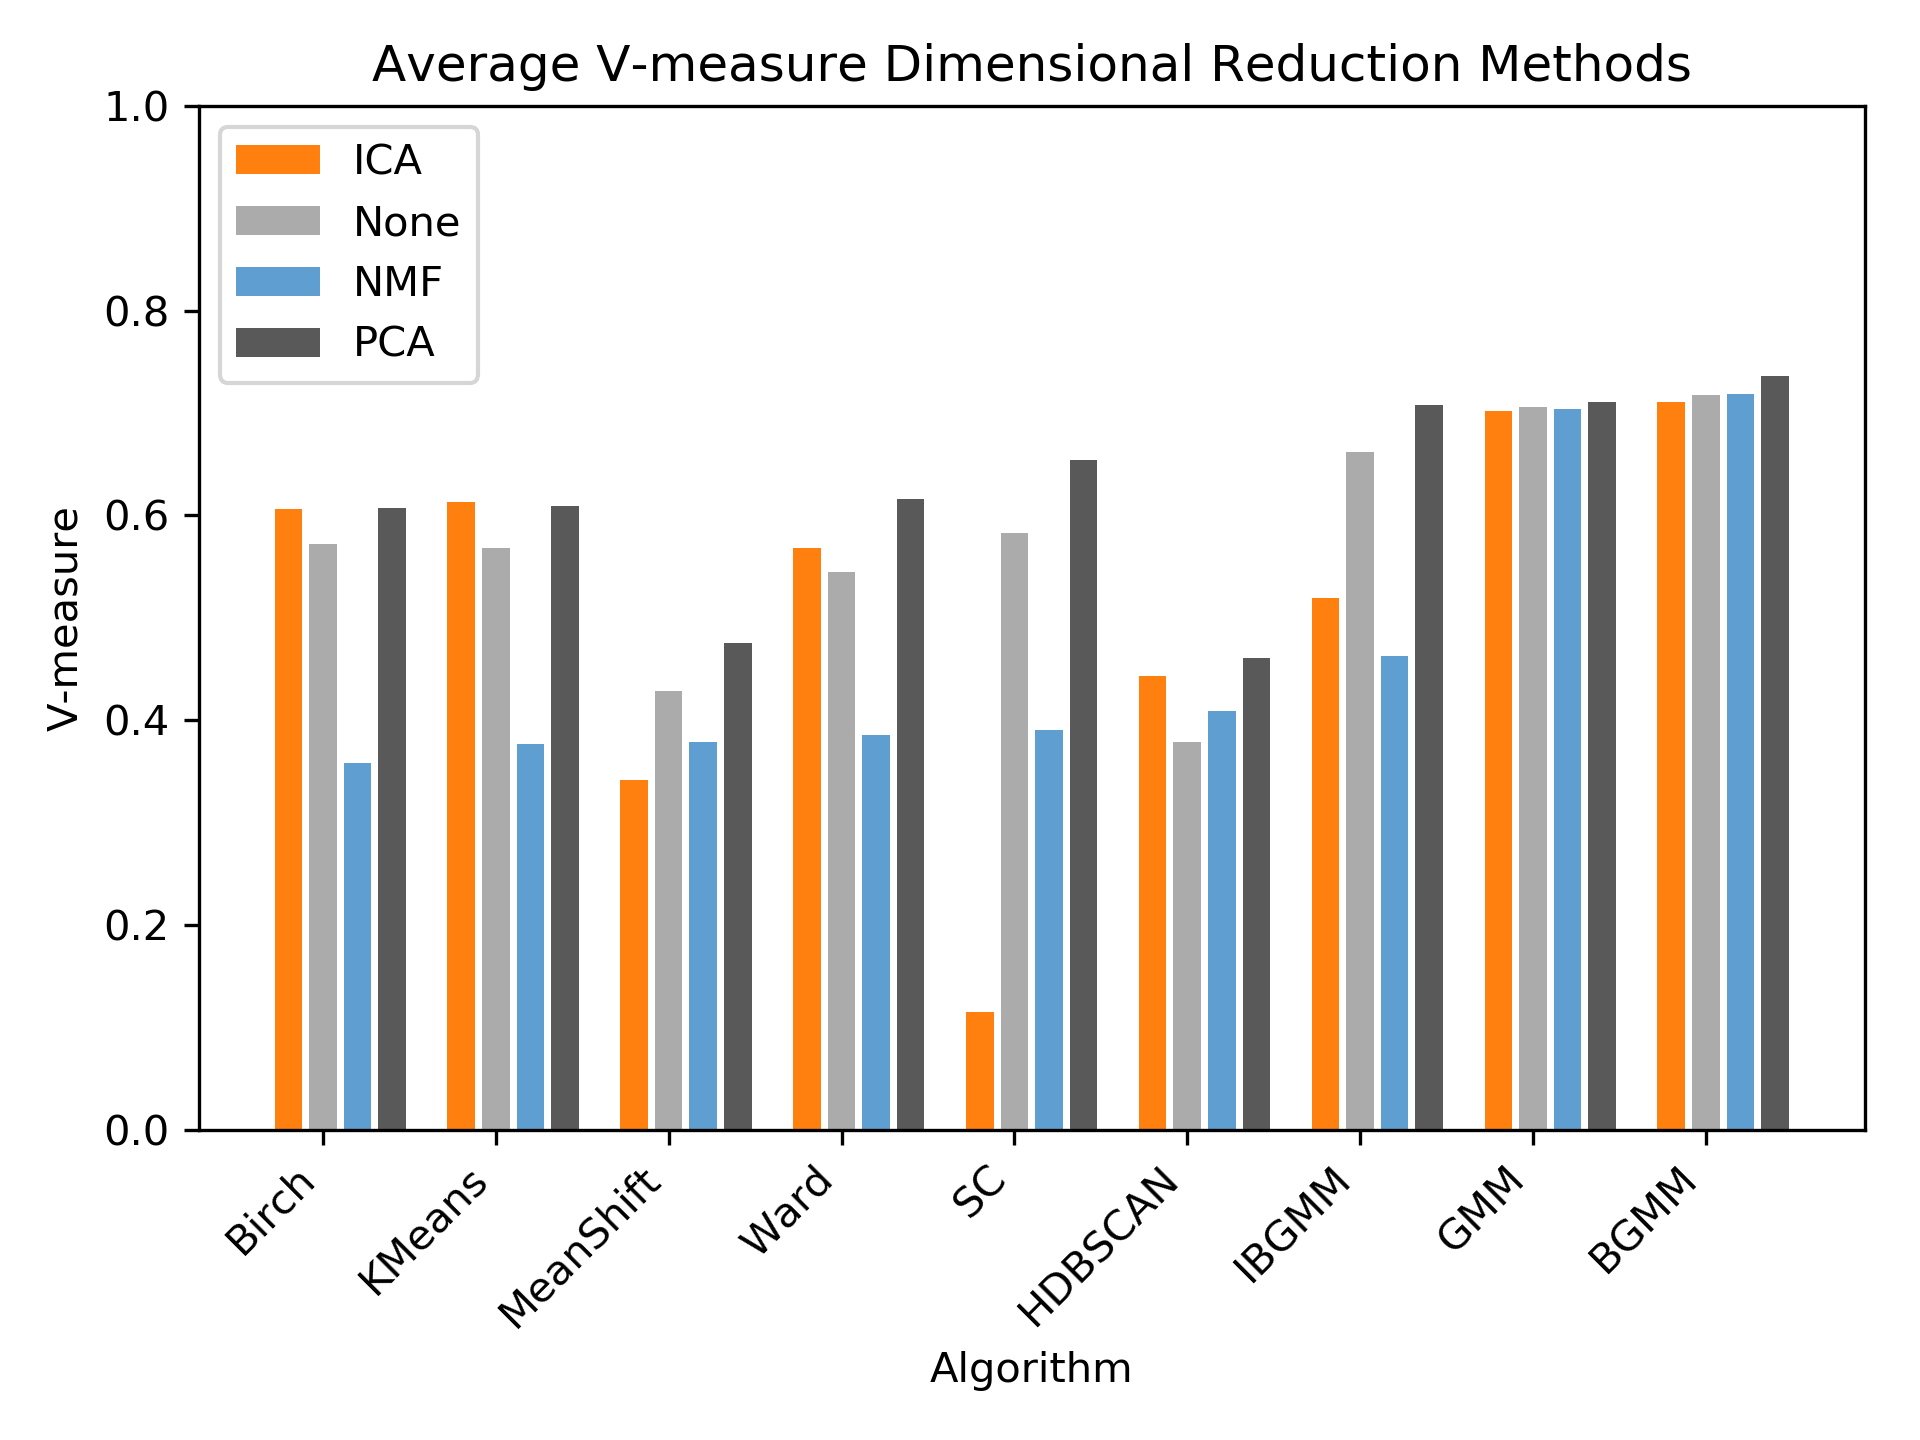
\includegraphics[width=0.48\textwidth]{figures/red_methods.png}
  \end{center}
  
  \caption{The first two non-negative factorization components of the data displayed as a scatter plot.}
  
  \label{results:dr}
\end{wrapfigure}

Figure \ref{results:hard_soft} a) shows the results of the clustering methods using PCA with two principal components. Overall the GMMs resulted in the best clustering V-measures. Spectral clustering resulted in comparable V-measure in some cases.

\begin{figure}[b!]
    \centering
    \begin{subfigure}[b]{0.32\textwidth}
        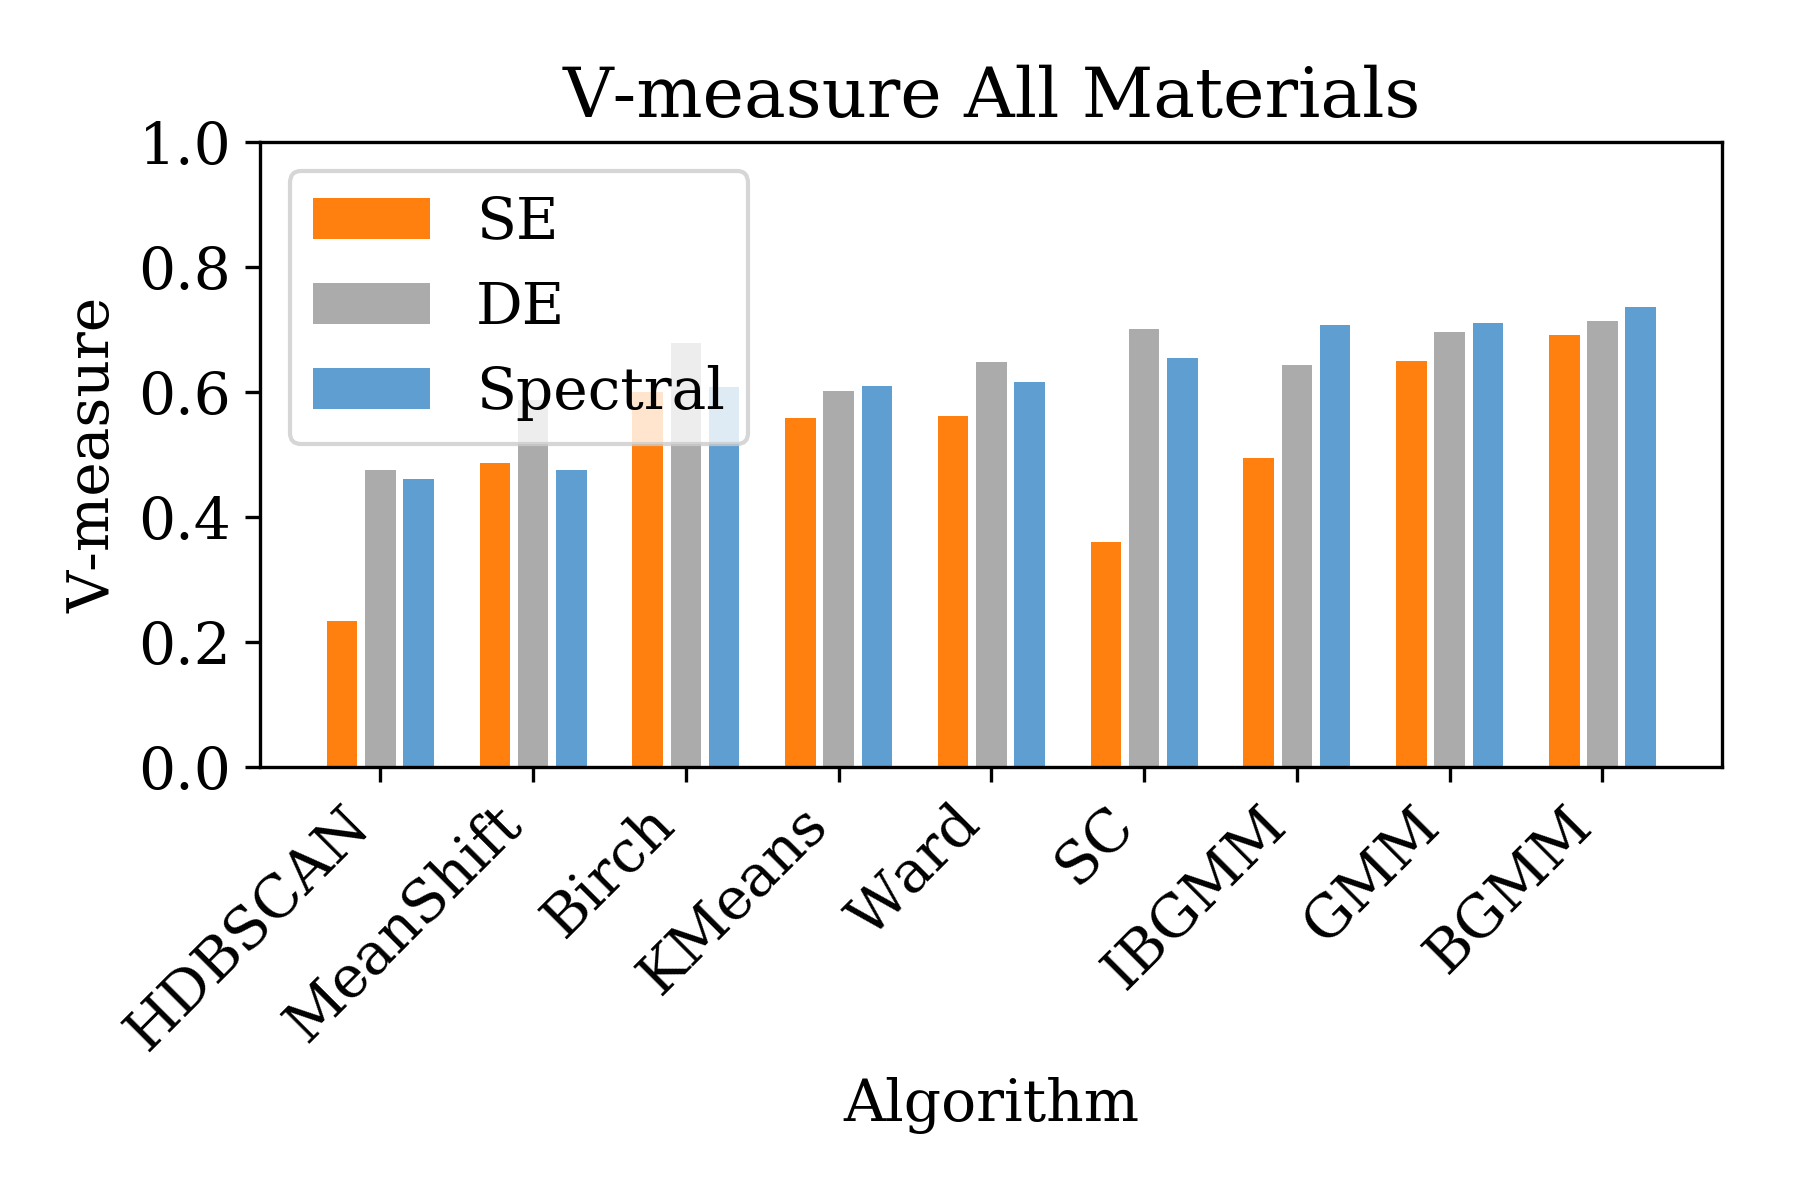
\includegraphics[width=\textwidth]{figures/energy_comparison.png}
    \end{subfigure}
    ~ %add desired spacing between images, e. g. ~, \quad, \qquad, \hfill etc. 
      %(or a blank line to force the subfigure onto a new line)
    \begin{subfigure}[b]{0.32\textwidth}
        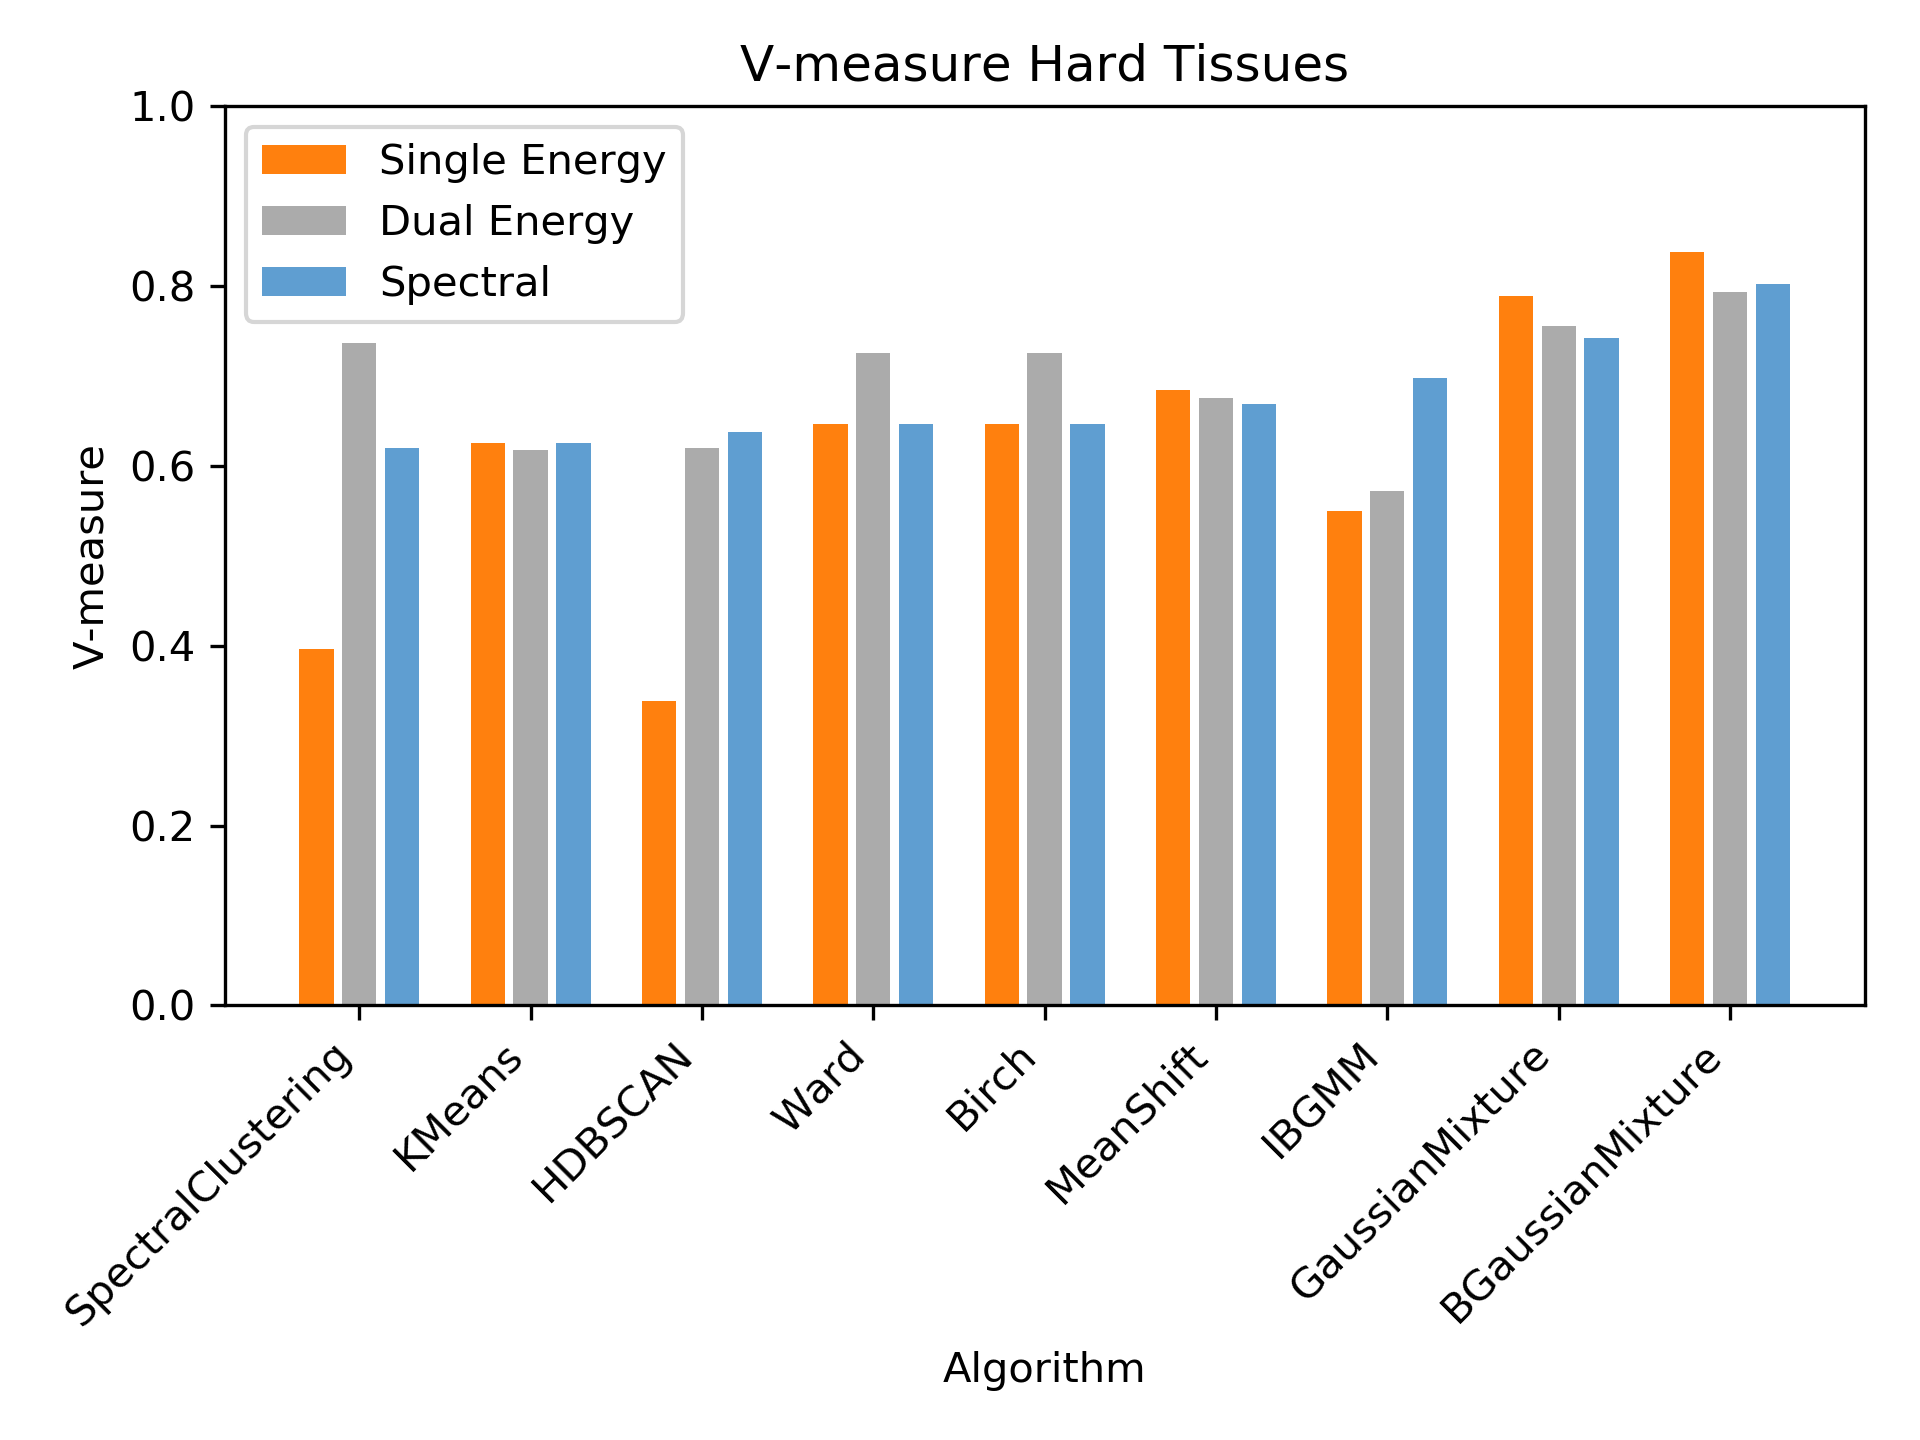
\includegraphics[width=\textwidth]{figures/hard.png}
    \end{subfigure}
    \begin{subfigure}[b]{0.32\textwidth}
        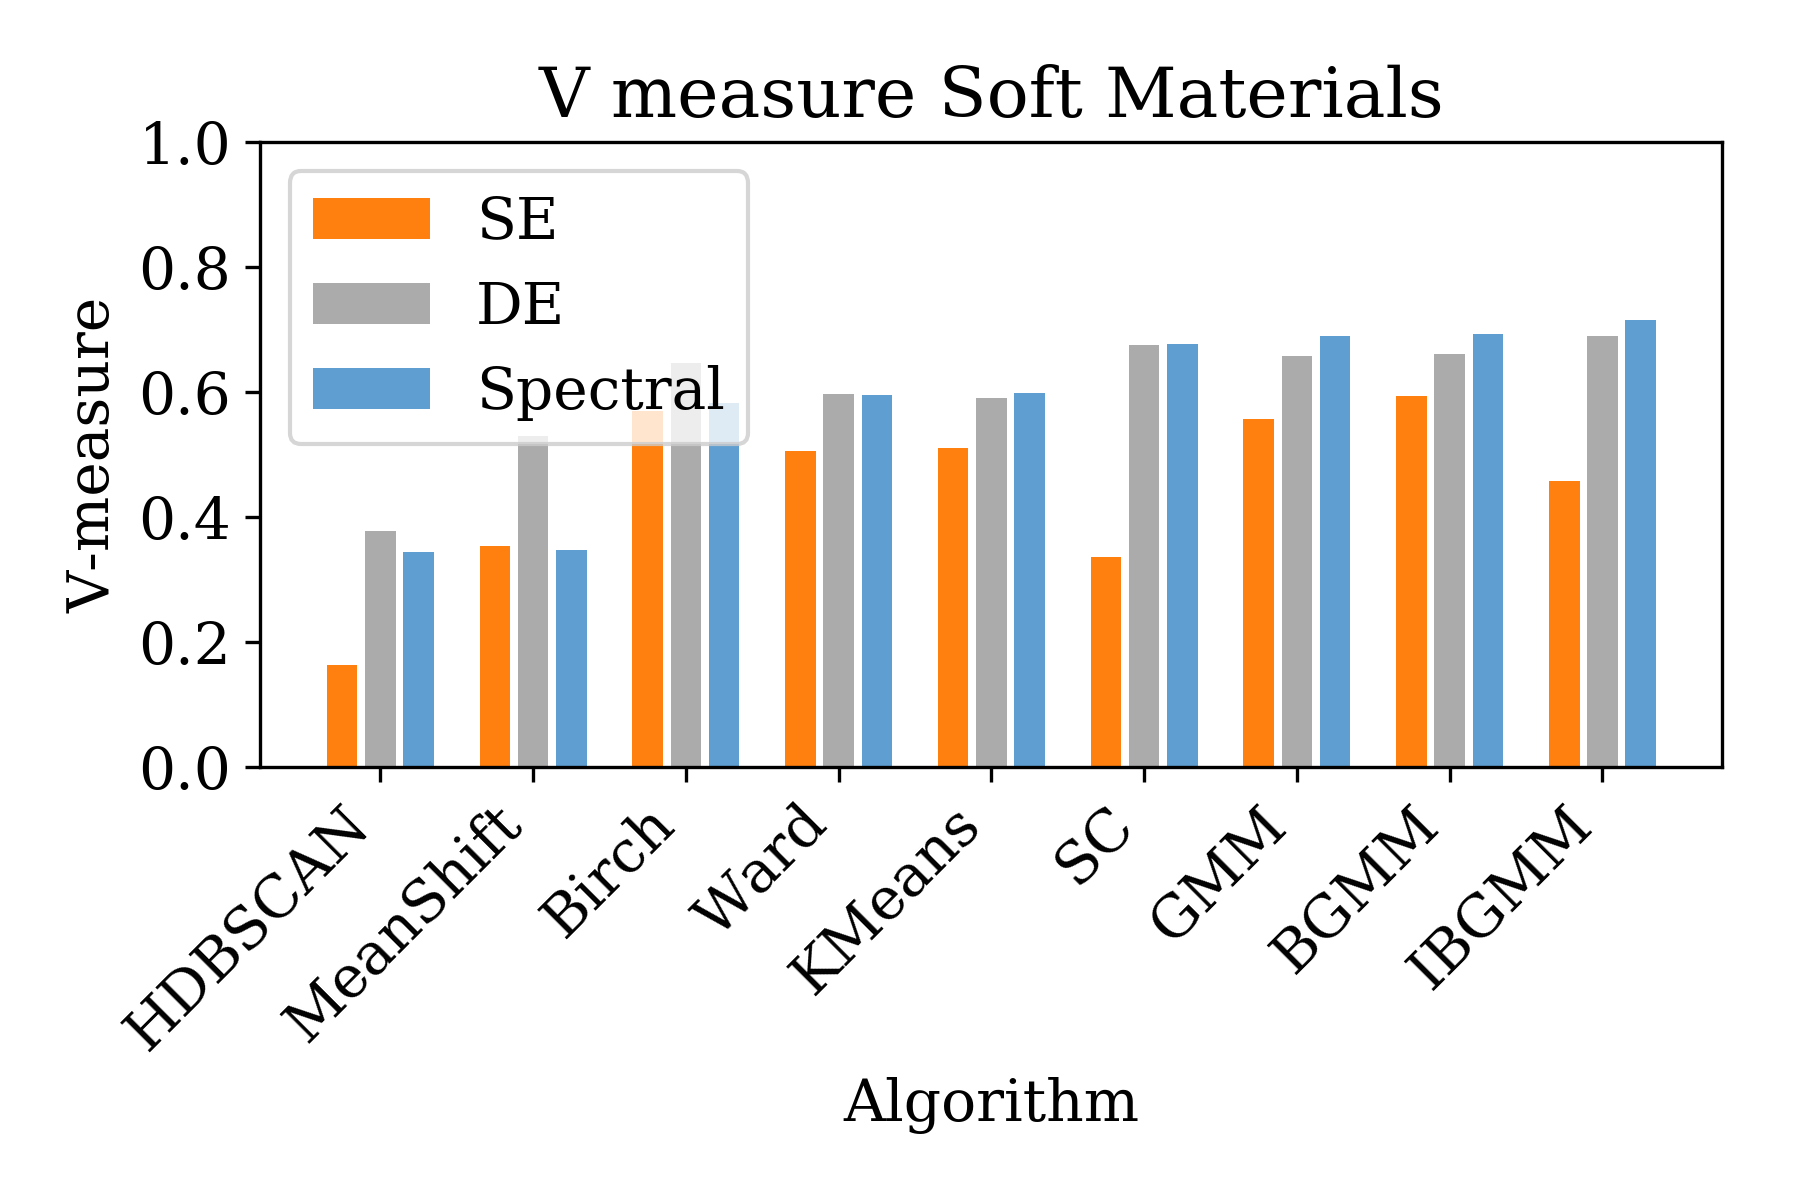
\includegraphics[width=\textwidth]{figures/soft.png}
    \end{subfigure}
    \caption{Clustering Methods}
    \label{results:hard_soft}
\end{figure}

\subsubsection{Comparison to Dual and Single Energy}

A dual energy image was created by summing over the first and last three bins of the image while a single energy image was created by summing over all of the bins. The clustering methods were applied to the two images and compared to the spectral image with PCA. Results can be seen in Figure \ref{results:hard_soft}.

Overall spectral imaging was seen to be marginally better that dual and single energy imaging averaged over all of materials. Spectral was \% better than dual energy imaging and \% better than single energy imaging.

Results differed significantly when looking at the soft tissue and hard tissue segmentations. Hard tissues were considered to be steel and glass while soft tissues were considered to be polypropylene, PTFE and bluebelt.

Figure \ref{results:hard_soft} b-c) show another dependence of the results. Namely, the results are highly dependant on the nature of the material being segmented. Hard materials such as glass and steel

\subsubsection{Number of Clusters}

Given the result that BGMMs result in the lowest V-measure, there is further analysis necessary to determine if the process can be automated completely. Namely if we can determine the number of clusters $k$ reliably without human oversight. This was attempted by comparing the AICs and weights for both the $k=1$ and $k=2$ cases. If the AIC did not decrease significantly between one and two clusters and the weights for the two clusters were similar this indicated that there was only one material present, this is known through the application of domain knowledge as if a sample were mostly the material were are trying to isolate, visual examination would likely be sufficient. 

The results for the multi-material phantom as well as for a blank scan of PCA are shown below. The AIC for all of materials was seen to decrease by \#\# and was seen to descrease by \#\# for the single material. The weights for the different materials were seen to be \% different in all cases and \% different in the one material case.

\begin{figure}[b!]
    \centering
    \begin{subfigure}[b]{0.48\textwidth}
        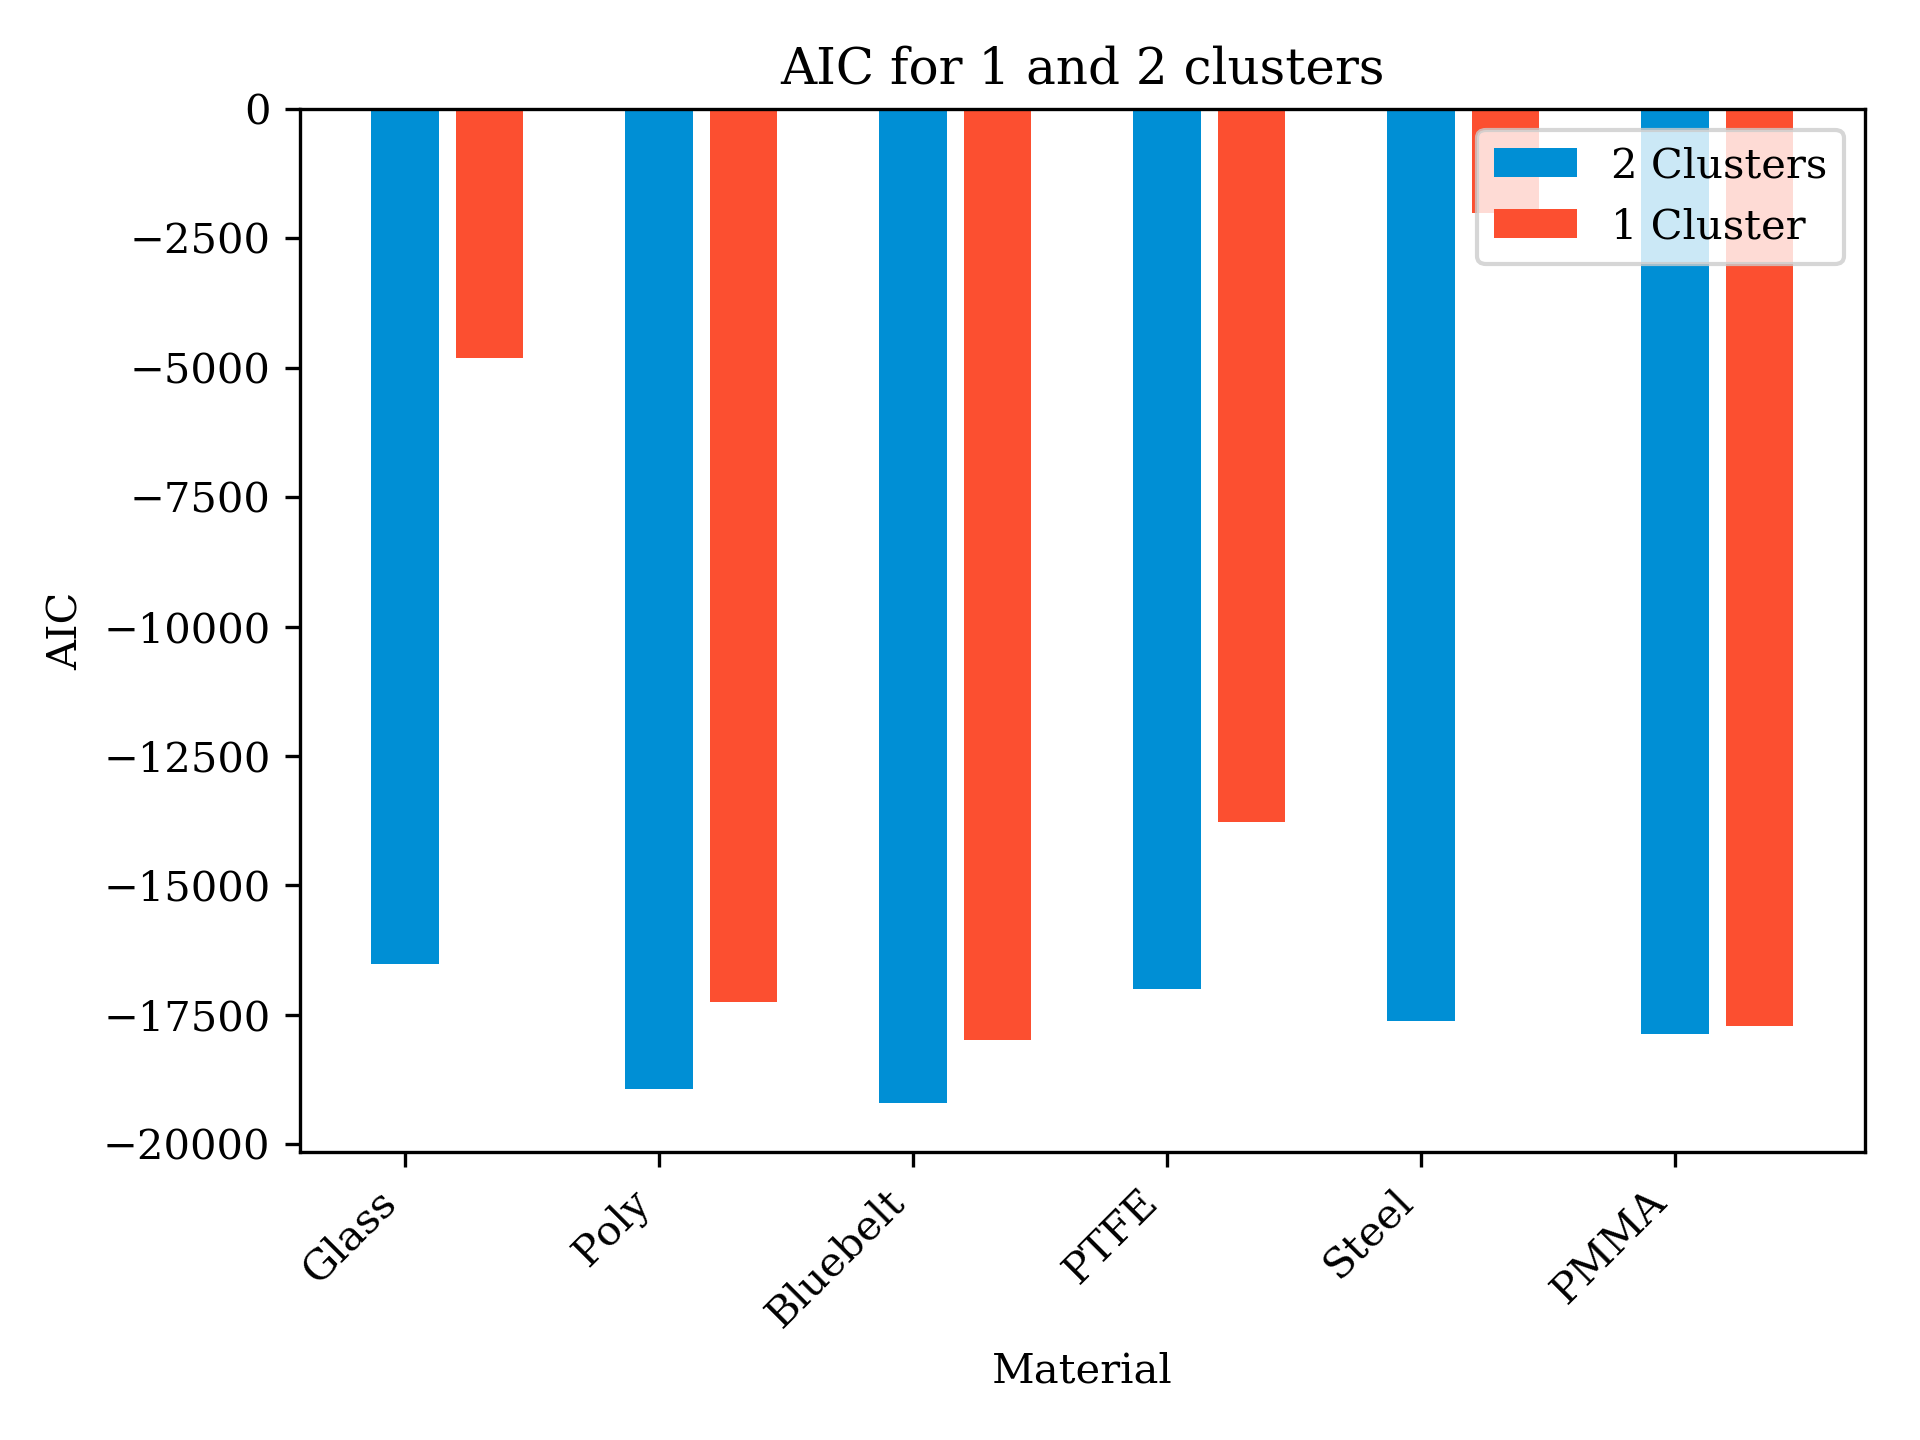
\includegraphics[width=\textwidth]{figures/AIC for 1 and 2 clusters.png}
    \end{subfigure}
    \begin{subfigure}[b]{0.48\textwidth}
        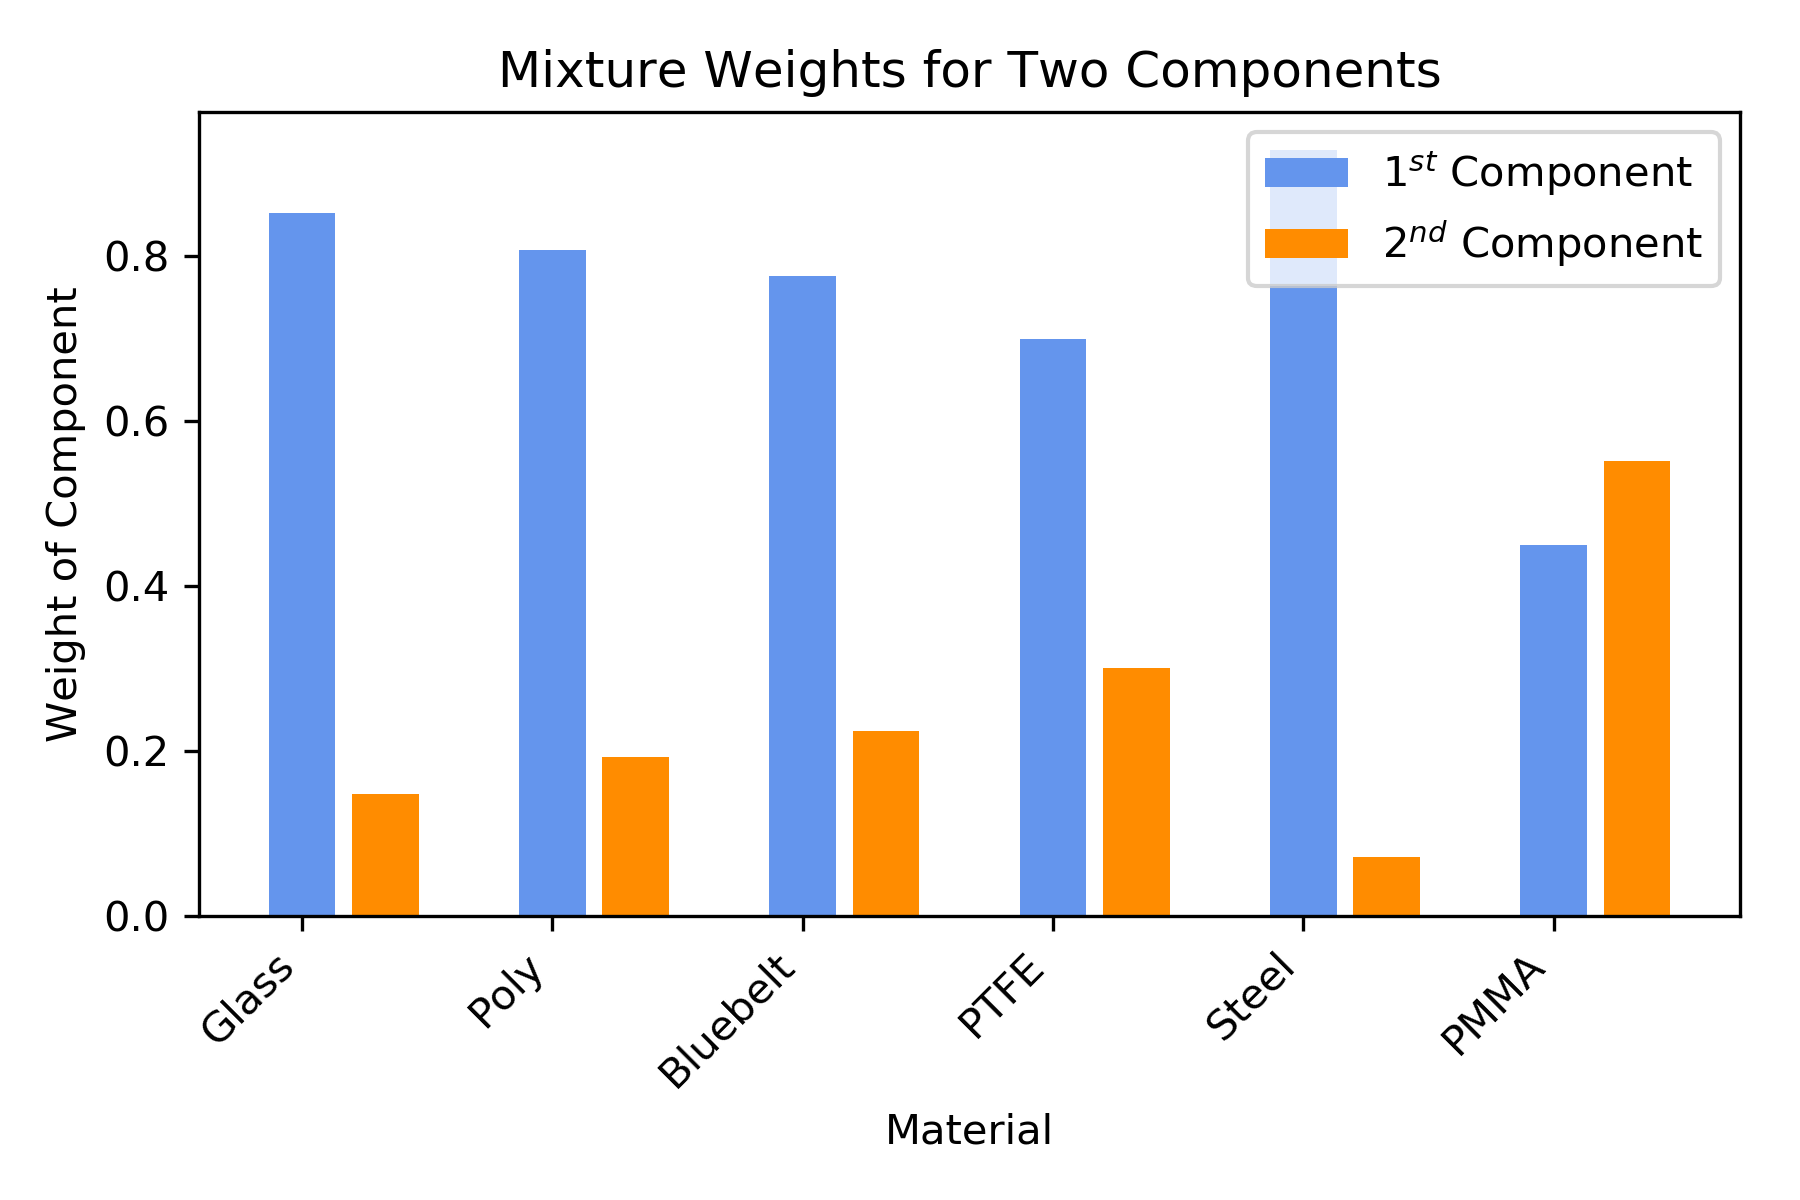
\includegraphics[width=\textwidth]{figures/weights.png}
    \end{subfigure}
    \caption{Clustering Methods}
    \label{n_bins}
\end{figure}

\subsubsection{Comparison to Otsu Thresholding}

In X-ray image segmentation Otsu's method is used often for image segmentation. Here we compare this algorithm to the IBGMM with spectral imaging on a soft tissue segmentation. Otsu's method overall had an average V-measure of \# however as can be seen in figure ??ref?? when the background had similar composition to the material in question there was erratic thresholding of the background. In this case the IBGMM had a V-measure of 0.74 while the thresholding method has a score of 0.41.

%--------------------------------------------------------------------------------%
%%%%%%%%%%%%%%%%%%%%%%%%%%%%%% Discussion %%%%%%%%%%%%%%%%%%%%%%%%%%%%%%%%%%%%
%--------------------------------------------------------------------------------%

\section{Discussion}

Machine learning has taken medical physics by storm. In recent years much work has been done implementing deep learning image segmentation. Deep learning implementations include considerable downfalls. It is known that these methods are only as good as their training data. To implement a successful deep learning model a large high quality dataset is needed. If the training data is does not completely cover the range of input in question it will behave erroneously.

In medical physics imaging modalities are constantly improving. The equipment of five or ten years ago often has different capabilities than the state of the art. Thus, having a machine learning system that is dependant on clinical data for training goes contrary to the development cycle of imaging modalities: Large clinical datasets will not be acquired until the modality has been adopted by a large amount of health care providers. This begs the question; if we are to implement new imaging modalities to leverage deep learning how do we validate their utility without large clinical datasets?

Thus this work is an alternate approach. Although the results of deep learning segmentation ??ref?? would likely result in superior segmentation. A clinical dataset for spectral imaging does not exist. If spectral imaging is put into clinical practice in coming years perhaps these datasets will exist. In the interim the IGMM method presented in this paper is the best candidate for soft tissue segmentation on these machines. This is of particular importance in spectra imaging since manual segmentation in is not as effective; clinicians are disadvantaged compared to a computer when dealing with five dimensional images as compared to flat images.

In summary, benchmarking of segmentation algorithms on dual, single, and spectral imaging has been presented as well as an improved method for image segmentation of soft materials in this domain. It was seen that single energy imaging is most capable of hard tissue segmentation having the highest V-measures on glass and steel separation tasks \#. While spectral imaging had the highest V-measure on the softer tissues.

It was seen that PCA is the optimal dimensional reduction method in this task. Although ICA shows promise in hyperspectral imaging, it did not show improvement over the unreduced data in this implementation. In the hyperspectral implementation however, domain knowledge was used to calculate the exact spectral response of the materials to be segmented. With an analytical detector response and a ray tracer we speculate that we could calculate a theoretical curve representing the signal produced by a material from out detector over all energy bins. With this knowledge we speculate that ICA could be a more effective method. PCA overall produced the best results over NMF, ICA and fully dimensional data. This was in part due to the use of spherical covariance in the GMMs for PCA, spherical covariance constrains the covariance to be the same in all dimensions for the fitted gaussians. Since PCA transforms the data into an basis with the two largest eigenvectors of the covariance orthogonal to each other spherical covariance was optimal. For NMF, ICA, and the complete data full covariance was used since spherical resulted in large overlaps.

For single energy imaging the GMM still showed the best results in this application.

One source of error in this paper was the use of a manual segmentation as a ground truth. Dividing the phantom into two materials made partial volume pixels a gray area as to which category they belonged. 

Meanshift, and hdbscan meant for more bins and fair that they fail in some cases since the definition of what a bin should be is loose. Spectral behaviour?

Fix the behaviour for the plots



%--------------------------------------------------------------------------------%
%%%%%%%%%%%%%%%%%%%%%%%%%%%%%% END %%%%%%%%%%%%%%%%%%%%%%%%%%%%%%%%%%%%
%--------------------------------------------------------------------------------%

\section*{Acknowledgments}

% or
\appendix{}
\section{Math}

To give a metric to describe the disorder in our clustering result we use the Shannon entropy of the classes given the clustering assignment $H(C|K)$ and the entropy of the classes  $H(C)$.

\begin{equation}
H(C|K) = - \sum_{c=1}^{|C|} \sum_{k=1}^{|K|} \frac{n_{c,k}}{n}
\cdot \log\left(\frac{n_{c,k}}{n_k}\right)
\end{equation}

\begin{equation}
H(C) = - \sum_{c=1}^{|C|} \frac{n_c}{n} \cdot \log\left(\frac{n_c}{n}\right)
\end{equation}

with $n$ the total number of data points, $n_c$ and $n_k$ the number of data points belonging to class $c$ and cluster $k$ respectively, and $n_{c,k}$ as the number of data points from class $c$ assigned to cluster $k$.

Rosenberg and Hirschberg then define the homogeneity $h$ and completeness $c$ as:

% \begin{equation}
    
% h = 1 - \frac{H(C|K)}{H(C)}

% c = 1 - \frac{H(K|C)}{H(K)}

% \end{equation}

In this study, methods were evaluated according to a combination of both homogeneity $h$ and completeness $c$. This combination is called the V-measure and is the harmonic mean of homogeneity and completeness.

\begin{equation}
v = 2 \cdot \frac{h \cdot c}{h + c}
\end{equation}

The components $x_i$ of the images with 5 bins $\boldsymbol{x}=(x_1,\ldots,x_5)^T$ are seen to be a sum of the independent components $s_k$, $k=1,\ldots,5$:

$x_i = a_{i,1} s_1 + \cdots + a_{i,k} s_k + \cdots + a_{i,5} s_5$

where $a_{i,k}$ are the mixing weights.

Or in matrix form as $\boldsymbol{x}=\sum_{k=1}^{5} s_k \boldsymbol{a}_k$, where our image vectors $\boldsymbol{x}$ are represented by the basis vectors $\boldsymbol{a}_k=(\boldsymbol{a}_{1,k},\ldots,\boldsymbol{a}_{m,k})^T$. The basis vectors $\boldsymbol{a}_k$ form the columns of the mixing matrix $\boldsymbol{A}=(\boldsymbol{a}_1,\ldots,\boldsymbol{a}_5)$.

Putting all this together we have the matrix equation $\boldsymbol{x}=\boldsymbol{A} \boldsymbol{s}$, where $\boldsymbol{s}=(s_1,\ldots,s_5)^T$.

Given our images $\boldsymbol{x}_1,\ldots,\boldsymbol{x}_N$ of the random vector $\boldsymbol{x}$, the task is to estimate both the mixing matrix $\boldsymbol{A}$ and the sources $\boldsymbol{s}$. This is done by adaptively calculating the $\boldsymbol{w}$ vectors and setting up a cost function which maximizes the non-gaussianity of the calculated $s_k = \boldsymbol{w}^T \boldsymbol{x}$. In this paper we use the maximum likelihood estimate (MLE) algorithm for finding the unmixing matrix $W$. 





\bibliographystyle{JHEP}
\bibliography{references2}


\vfill





%Removed by Kevin%
%This work aims to examine the potential of spectral imaging in nondestructive testing (DNT) what the minimal imaging parameters are for systems to be accurate. Specifically, to examine the detection of different thicknesses of cartilage under different xray exposures. To this aim, the independent variables in question will be signal to noise ratio (SNR) and thickness of cartilage in cm. The novelty of this work is twofold: The first novel component is a REDLEN cadmium zinc telluride semiconductor PCD. Secondly, the cartilage identification method is novel in that it extends dual energy extraction of Alvarez [3] to many energies. This method is coupled with a convolutional neural network (CNN) , the architecture being the U-Net achitecture which is shown to be optimal for segmentation [4]. And has also been used in k-edge imaging for spectral CT [5] Overall, this work aims to examine the application of CNNs and photon counting detectors (PCDs) in planar medical imaging.






% Can be used to pull up biographies so that the bottom of the last one
% is flush with the other column.
%\enlargethispage{-5in}



% that's all folks
\end{document}
% \title{Journal of Instrumentation (JINST) template}


% %% %simple case: 2 authors, same institution
% %% \author{A. Uthor}
% %% \author{and A. Nother Author}
% %% \affiliation{Institution,\\Address, Country}

% % more complex case: 4 authors, 3 institutions, 2 footnotes
% \author[a,b,1]{F. Irst,\note{Corresponding author.}}
% \author[c]{S. Econd,}
% \author[a,2]{T. Hird\note{Also at Some University.}}
% \author[c,2]{and Fourth}

% % The "\note" macro will give a warning: "Ignoring empty anchor..."
% % you can safely ignore it.

% \affiliation[a]{One University,\\some-street, Country}
% \affiliation[b]{Another University,\\different-address, Country}
% \affiliation[c]{A School for Advanced Studies,\\some-location, Country}

% % e-mail addresses: only for the corresponding author
% \emailAdd{first@one.univ}



% \abstract{Abstract...}



% \keywords{Only keywords from JINST's keywords list please}


% \arxivnumber{1234.56789} % only if you have one


% % \collaboration{\includegraphics[height=17mm]{example-image}\\[6pt]
% %   XXX collaboration}
% % or
% \collaboration[c]{on behalf of XXX collaboration}


% % if you write for a special issue this may be useful





% \begin{document}
% \maketitle
% \flushbottom

% \section{Introduction}
% \label{sec:intro}

% The modern production line seeks efficiency through automation of human roles. When used properly, automation can increase production and lower cost. With automation, however, comes an increased pressure on quality control: Machines, unlike humans, are not expected to know if the product is contaminated by their actions. The ideal quality control in these situations is what is known as nondestructive testing (NDT), testing that leaves the product unchanged. The ideal NDT method is the use of XRay imaging. Current XRay imaging capabilities are limited to the detection of large differences in material density. However, new photon count detectors (PCDs) allow for XRay imaging to be extended to materials of similar composition. This application is particularly important in the meat processing industry where cartilage and tissue share similar compositions.

% In this work, spectral imaging is examined for the detection of cartilage in soft tissue. This is meant to be a direct application to the poultry industry. However, these results apply equally to the planar XRay discrimination of other materials with two components of similar composition. Other works have been done to investigate dual energy imaging in this application (???), but the extension to more energies has not been seen.

% It is important to note some other considerations in this problem: Firstly, this system must image objects on a conveyor belt moving at 0.5 m/s. And secondly to be cost effective the xray tube should be one with low current. Thus when discussing this problem it is essential to look at xray imaging for a photon starved system. 

% This work aims to examine exactly what the minimal imaging parameters are for systems to be accurate. Specifically, to examine the detection of different thicknesses of contaminant under different xray exposures. To this aim, the independent variables in question will be signal to noise ratio (SNR) and thickness of cartilage in cm.

% The novelty of this work is twofold: The first novel component is the modeling of a REDLEN cadmium zinc telluride semiconductor PCD. Secondly, the cartilage identification method is novel in that it extends dual energy extraction of (???) to many energies. This method is coupled with a convolutional neural network (CNN) , the architecture being the U-Net achitecture which is shown to be optimal for segmentation. Overall, this work aims to examine the application of CNNs and photon counting detectors (PCDs) in nondestructive imaging.

% \section{Methods}
% \label{sec:methods}

% An overview of the total work flow can be seen in figure~\ref{fig:i}:


% \begin{figure}[htbp]
% \centering % \begin{center}/\end{center} takes some additional vertical space
% \includegraphics[width=\textwidth]{figures/Slide4.jpg}
% \qquad
% % "\includegraphics" from the "graphicx" permits to crop (trim+clip)
% % and rotate (angle) and image (and much more)
% \caption{\label{fig:i} Complete work flow U-Net image reproduced with permission (???) from ....}
% \end{figure}

% Steps 1 (Image Simulation) and 2 (Multi-Energy Subtraction) are used to optimize the imaging parameters while the third step (Image Segmentation and Classification) is used to determine the limitations of the higher level classification.

% \subsection{Image Simulation}
% \subsubsection{Phantoms, Spectra and General Parameters}

% The phantoms used in this study were composed of Cartilage and Solid Water, the exact composition of the cartilage follows the ICRU-44 guidelines and the water is that of Watanabe 1999. 

% Table(*???)

% Three seperate phantoms were modeled of three diferent water thickness 8,  6, and 4 cm respectively. These thicknesses were chosen to span the range of thicknesses expected in the calibration, smaller phantoms were investigated but resulted in less failure of differentiation. In this phantom smaller inserts of 0:4 cm in 0.5cm increments were embedded, it is noted that the best interpolation would be the use of the Chebyshev nodes for this range as proposed by (???) however it has also been demonstrated that machinists prefer lengths that are rational numbers.

% \begin{figure}[htbp]
% \centering % \begin{center}/\end{center} takes some additional vertical space
% 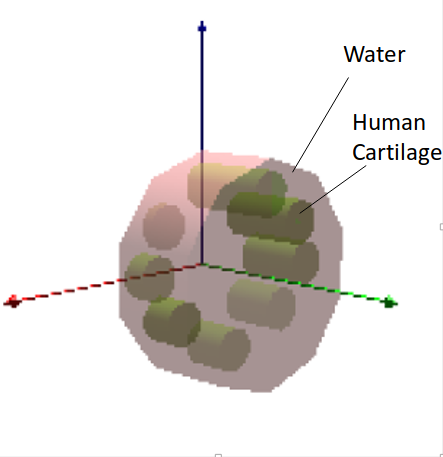
\includegraphics[width=0.4\textwidth]{figures/phantom.png}
% \qquad
% 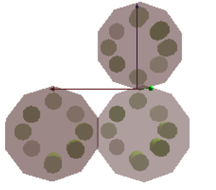
\includegraphics[width=.4\textwidth,]{figures/phantom3.png}
% % "\includegraphics" from the "graphicx" permits to crop (trim+clip)
% % and rotate (angle) and image (and much more)
% % "\includegraphics" from the "graphicx" permits to crop (trim+clip)
% % and rotate (angle) and image (and much more)
% \caption{\label{fig:i}  An image of one of the phantoms and all three}
% \end{figure}

% A similar phantom was used for the validation step save but with inserts of 0.4:3.9 cm in 0.5 cm increments.

% The spectra used was a simple 60 kVp spectrum with generated from a tungsten anode with 0.8 mm beryllium, 30 cm air and 0.1 mm copper filtration. The detector was an ideal integrating detector over the energy range indicated 

% A note should be made on the binning of the energies, energy bins for all of the simulation were calculated so as to have equal fluency in the each energy bin. These bins were calculated by integrating over the desired fraction of the spectra. This was done for optimal statistics as noise increases quadratically with decreasing signal equal fluence results in the best average signal to noise in the images. 

% \subsubsection{Analytical}

% Two separate types of simulations were preformed in this work, the first image simulation method uses Imasim (???) a ray tracing application that provides perfect ray tracings, Gaussian random noise was added to the images to mimic the Poisson statistics that occur in a normal image, the imaging parameters were made to the specifications of the REDLEN detector :

% table()

% \subsubsection{Monte Carlo}

% A monte carlo simulation was done using Geant4 extended by TOPAS, the spectrum was sampled from a analytically simulating with 89 points sampled over the spectra. For each phantom thickness 10 trials were preformed with different random number seeds with 5000000 photons each, these trails were summed to make up the images with the different signals. Complete imaging parameter files can be found in the github repository.


% \subsection{Multi-Energy Subtraction}


% Alvarez et al. mention many times in various papers that there is no improvement to dual energy subtraction when using more energies. This stems from the fact that the photoelectric component and the compton scattering component of the photon interactions fully describe the system, therefore two components can span this space and further images will just give linearly dependant information. In less words;



% \begin{equation}
% \label{eq:1}
% \mu(x,y,E) = a_1(x,y) \frac{1}{E^3}+a_2(x,y) f_{KN}(E)
% \end{equation}

% Where x, y and E need no explanation $\mu$ is the attenuation and $a_1, a_2 $ are coefficients for the photoelectric effect and Compton scattering component and $f_{KN}(E)$ is the Klein-Nishina function.

% However the finding of these coefficients is generally left to a least squares fitting of the material thicknesses $A_1, A_2$ to the log intensity $I_{energy 1}, I_{energy 2}$ of the image to find the parameters ${k_n}, {l_n}$ (ref ref ref???)


% \begin{subequations}\label{eq:t}
% \begin{align}
% \label{eq:t:1}
%  \ln(I_{energy 1}) = k_1 A_1 + k_2 A_2 +k_3A_1^2 +k_4 A_2^2 +k_5 A_1A_2 
% \\
% \label{eq:t:2}
% \ln(I_{energy 2}) = l_1 A_1 + l_2 A_2 +l_3A_1^2 +l_4 A_2^2 +l_5 A_1A_2 
% \end{align}
% \end{subequations}

% However this practise is not likely to produce the intended parametrization of the intensity of the image as a function of the Compton scattering and Photoelectric effect, instead is mush more likely to fit to the pixel intensity. To give an example, a least squares fit of thickness of bone $(A_1)$ and brain $(A_2)$ to one image will generate fit coefficients that map pixel intensity to bone thickness, since one cannot parametrize decompose an image into compton scattering and photoelectric effect in one image. This demonstrates that there is other information for the least squares fit to calibrate on. Given this it is safe to assume that when given more images the coefficients still have the possibility of fitting based off of the intensity rather than the CS/PE. Since the fit is not based entirely off of CS/PE it is possible that more images will give a better fit that will be based more on the CS/PE components in the material and less on the raw pixel intensity.

% Thus the idea of more energies being unececessary was put on hold and \ref{eq:y} was bravely extended to n energies as

% \begin{subequations}\label{eq:p}
% \begin{align}
% \label{eq:p:1}
% A_1 = \sum_{m=1}^n k_{m} \ln(I_{m})  +\sum_{j=1}^n  k'_{j,m} \ln(I_{j}) \ln(I_{m})
% \\
% \label{eq:p:2}
% A_2 = \sum_{m=1}^n l_{m} \ln(I_{m})  +\sum_{j=1}^n  l'_{j,m} \ln(I_{j}) \ln(I_{m})
% \end{align}
% \end{subequations}


% \subsubsection{Least-Squares Fitting}

% The least squares regression used was similar to what is described in \ref{eq:p} extended to n energies
% the intensities used in the fit were taken from the circular inserts of the phantom.

% \subsubsection{Non-Linear Fitting}

% The same equation \ref{eq:p} was fit using a feed forward neural network (MATLAB feedforwardnet(???)), the hyper parameters used were the defaults save the number of hidden layers was optimized individually for each combination of SNR by running 10 trials each for 5 to 100 layers in 5 layer interval, the optimal amount of layers was then selected as the result with the lowest mean squared error MSE on the validation data.

% \subsection{Image Segmentation and Classification}

% The input for the CNN is generated randomly assigned polygons as the background, these polygons are assigned image values taken from the validation images in Imasim with Poisson noise added to get the desired signal to noise ratio. The background polygons are composed of water in this way. The foreground is composed of circular regions of differing thicknesses of combined water and cartilage again taken from the Imasim validation data set, the U-Net is also provided a segmentation for training as seen in figure \ref{fig:j}. The exact hyperparameters for the network can be found at github (???).


% \begin{figure}[htbp]
% \centering % \begin{center}/\end{center} takes some additional vertical space
% 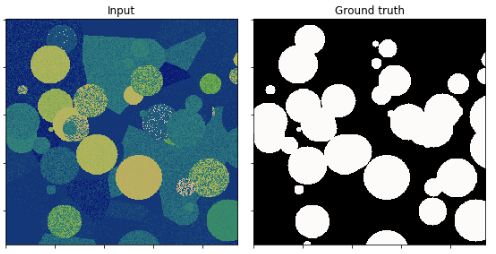
\includegraphics[width=\textwidth]{figures/CNN_val.png}
% \qquad
% % "\includegraphics" from the "graphicx" permits to crop (trim+clip)
% % and rotate (angle) and image (and much more)
% \caption{\label{fig:j} Complete work flow U-Net image reproduced with permission (???) from ....}
% \end{figure}

% \section{Results}

% The linear and non-linear regression were evaluated by means of CNR, MSE as a function of amount cartilage ($T_c$) and SNR. With the CNR and SNR defined relative to 4cm of water, specifically

% \begin{equation}
% \label{eq:f}
% CNR = \frac{|I^m_{ROI} - I^m_{H_2O}|}{\sqrt{\sigma^2_{ROI} + \sigma^2_{H_2O}}}
% \end{equation}
% The CNR was bootstrapped to the 95\% confidence interval which is shown as a band in figure ??ref??

% If you want some equations without the tag (number), please use the available
% starred-environments. For example:
% \begin{equation*}
% x = 1
% \end{equation*}

% The amsmath package has many features. For example, you can use use
% \texttt{subequations} environment:
% \begin{subequations}\label{eq:y}
% \begin{align}
% \label{eq:y:1}
% a & = 1 
% \\
% \label{eq:y:2}
% b & = 2
% \end{align}
% and it will continue to operate across the text also.
% \begin{equation}
% \label{eq:y:3}
% c = 3
% \end{equation}
% \end{subequations}
% The references will work as you'd expect: \eqref{eq:y:1},
% \eqref{eq:y:2} and \eqref{eq:y:3} are all part of \eqref{eq:y}.

% A similar solution is available for figures via the \texttt{subfigure}
% package (not loaded by default and not shown here).
% All figures and tables should be referenced in the text and should be
% placed on the page where they are first cited or in
% subsequent pages. Positioning them in the source file
% after the paragraph where you first reference them usually yield good
% results. See figure~\ref{fig:i} and table~\ref{tab:i}.

% \begin{figure}[htbp]
% \centering % \begin{center}/\end{center} takes some additional vertical space
% \includegraphics[width=.4\textwidth,trim=30 110 0 0,clip]{example-image-a}
% \qquad
% \includegraphics[width=.4\textwidth,origin=c,angle=180]{example-image-b}
% % "\includegraphics" from the "graphicx" permits to crop (trim+clip)
% % and rotate (angle) and image (and much more)
% \caption{\label{fig:i} Always give a caption.}
% \end{figure}


% \begin{table}[htbp]
% \centering
% \caption{\label{tab:i} We prefer to have borders around the tables.}
% \smallskip
% \begin{tabular}{|lr|c|}
% \hline
% x&y&x and y\\
% \hline
% a & b & a and b\\
% 1 & 2 & 1 and 2\\
% $\alpha$ & $\beta$ & $\alpha$ and $\beta$\\
% \hline
% \end{tabular}
% \end{table}

% We discourage the use of inline figures (wrapfigure), as they may be
% difficult to position if the page layout changes.

% We suggest not to abbreviate: ``section'', ``appendix'', ``figure''
% and ``table'', but ``eq.'' and ``ref.'' are welcome. Also, please do
% not use \texttt{\textbackslash emph} or \texttt{\textbackslash it} for
% latin abbreviaitons: i.e., et al., e.g., vs., etc.



% \section{Sections}
% \subsection{And subsequent}
% \subsubsection{Sub-sections}
% \paragraph{Up to paragraphs.} We find that having more levels usually
% reduces the clarity of the article. Also, we strongly discourage the
% use of non-numbered sections (e.g.~\texttt{\textbackslash
%   subsubsection*}).  Please also see the use of
% ``\texttt{\textbackslash texorpdfstring\{\}\{\}}'' to avoid warnings
% from the hyperref package when you have math in the section titles



% \appendix
% \section{Some title}
% Please always give a title also for appendices.





% \acknowledgments

% This is the most common positions for acknowledgments. A macro is
% available to maintain the same layout and spelling of the heading.

% \paragraph{Note added.} This is also a good position for notes added
% after the paper has been written.





% % We suggest to always provide author, title and journal data:
% % in short all the informations that clearly identify a document.

% \begin{thebibliography}{99}

% \bibitem{a}
% Author, \emph{Title}, \emph{J. Abbrev.} {\bf vol} (year) pg.

% \bibitem{b}
% Author, \emph{Title},
% arxiv:1234.5678.

% \bibitem{c}
% Author, \emph{Title},
% Publisher (year).


% % Please avoid comments such as "For a review'', "For some examples",
% % "and references therein" or move them in the text. In general,
% % please leave only references in the bibliography and move all
% % accessory text in footnotes.

% % Also, please have only one work for each \bibitem.


% \end{thebibliography}
% \end{document}
% \begin{figure}
%     \centering
%     \begin{subfigure}[b]{0.3\textwidth}
%         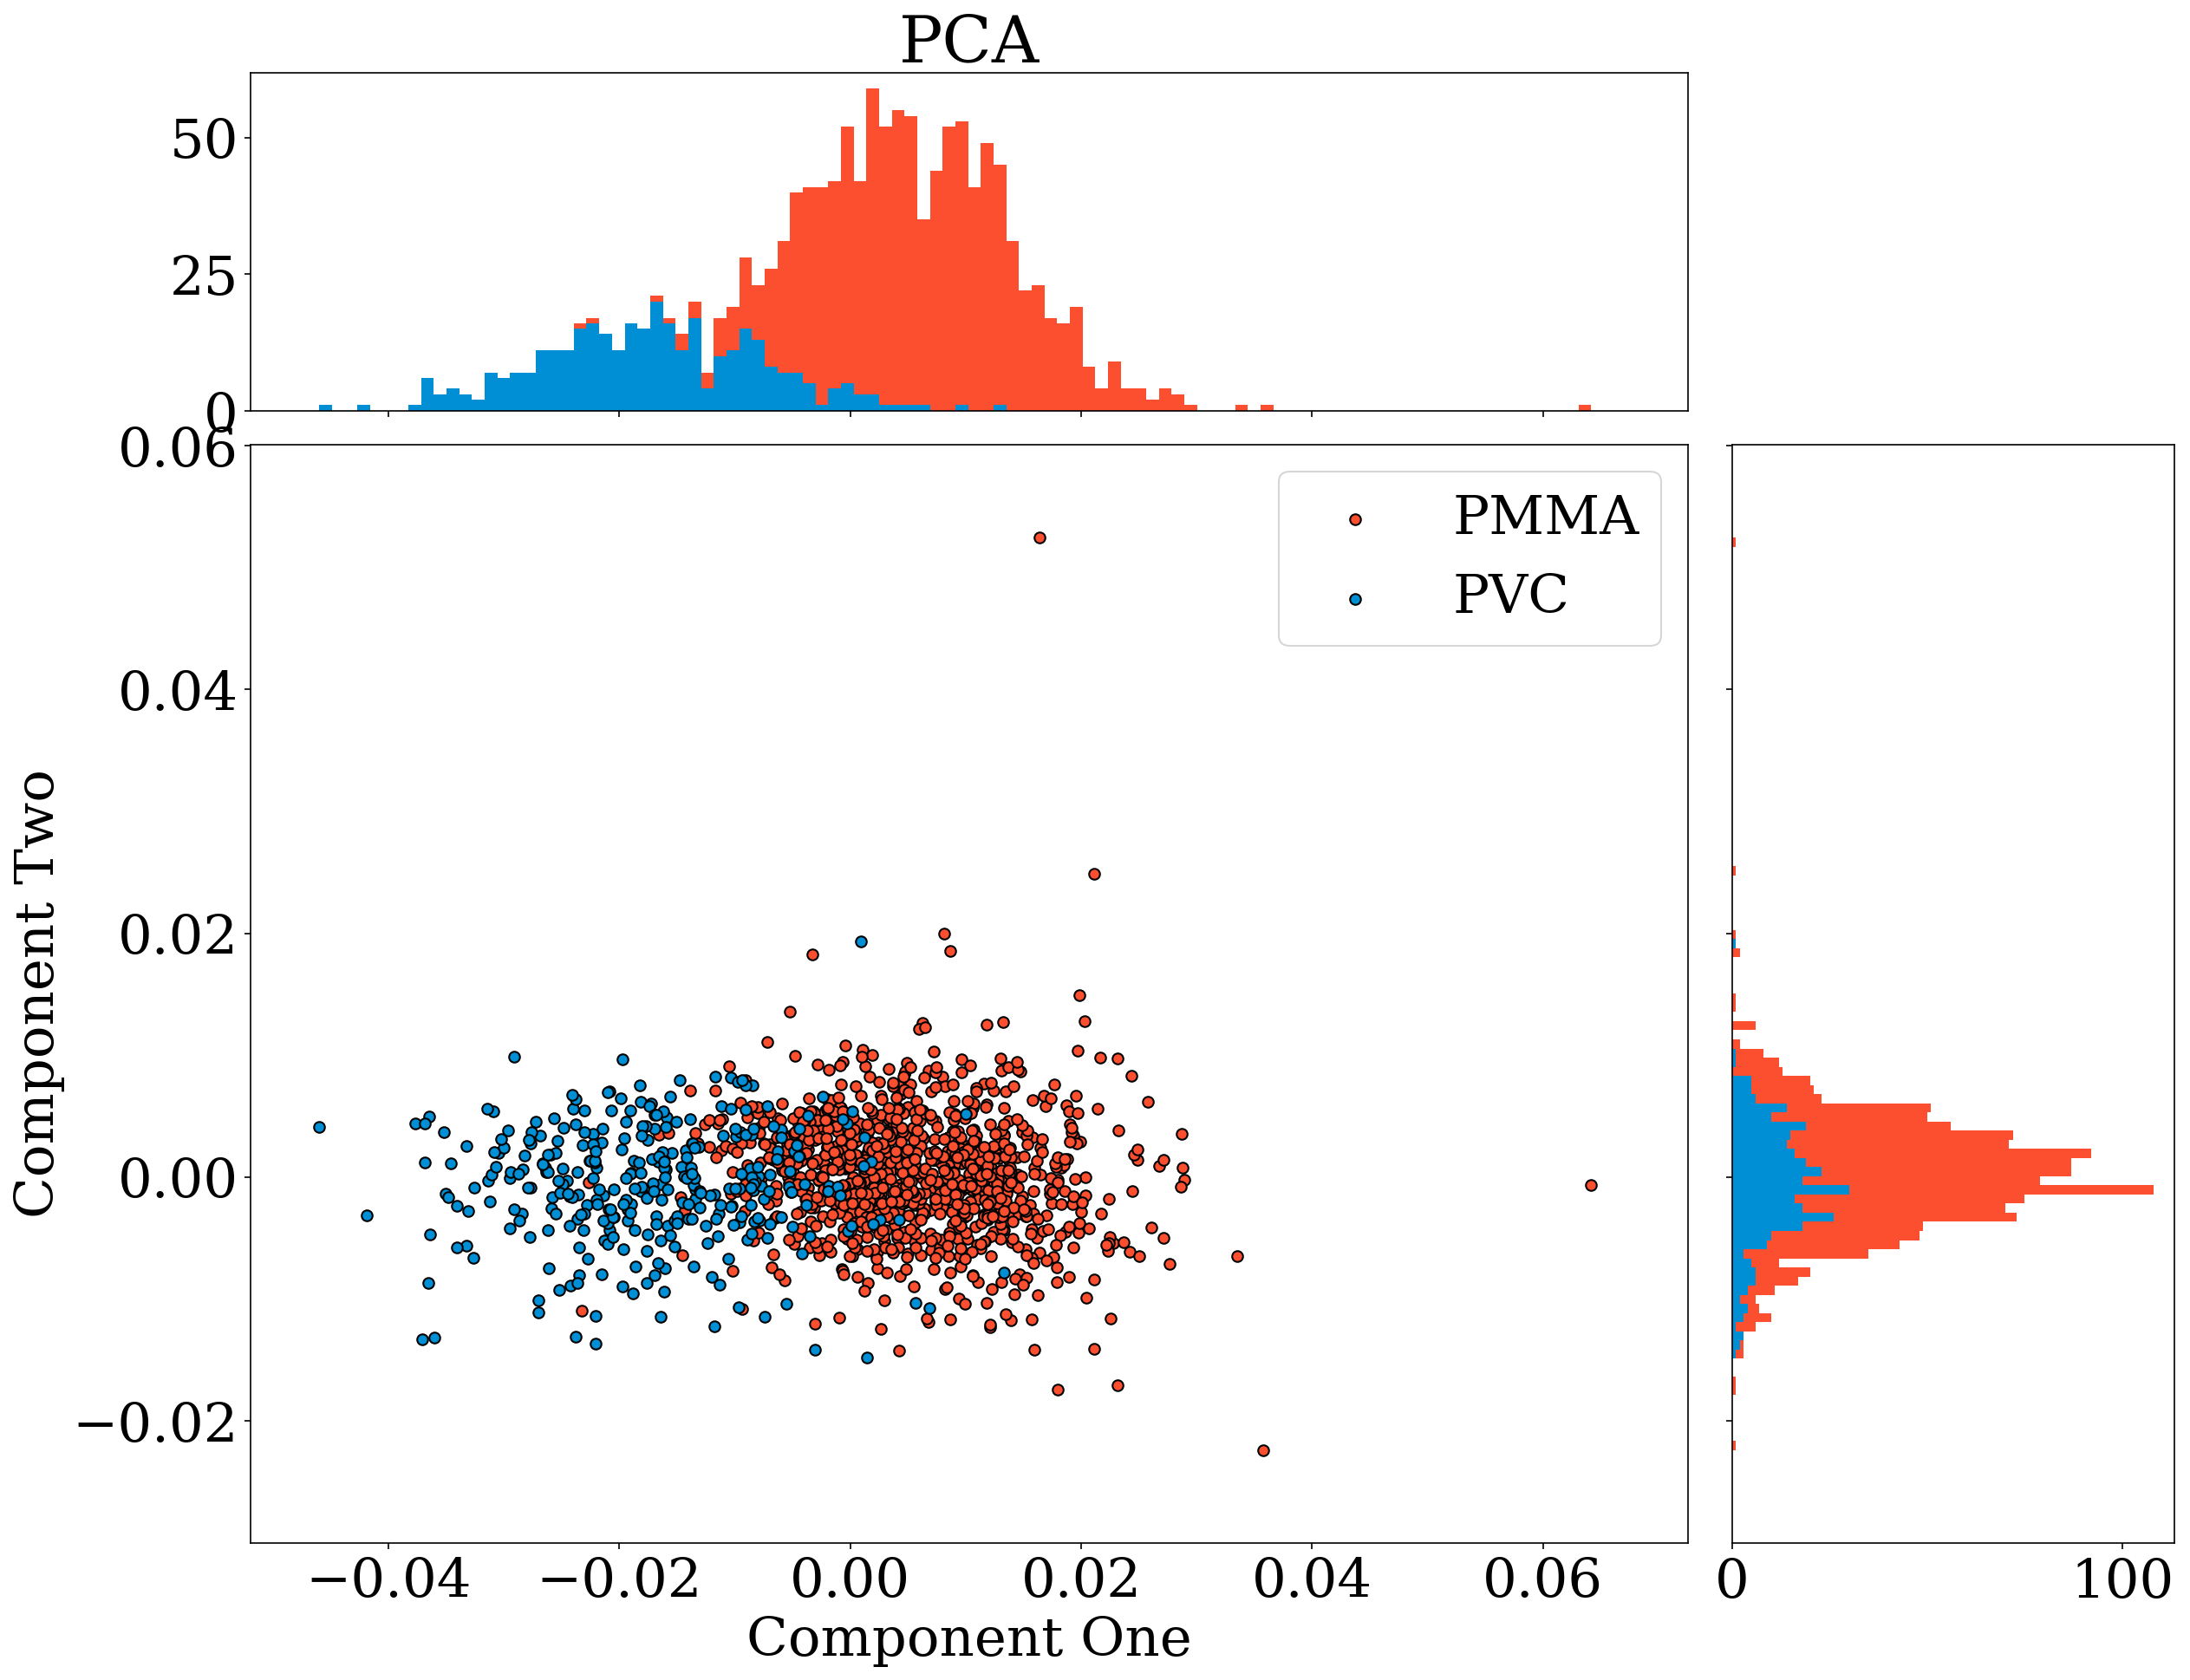
\includegraphics[width=\textwidth]{figures/PCAnone.png}
%     \end{subfigure}
%     ~ %add desired spacing between images, e. g. ~, \quad, \qquad, \hfill etc. 
%       %(or a blank line to force the subfigure onto a new line)
%     \begin{subfigure}[b]{0.3\textwidth}
%         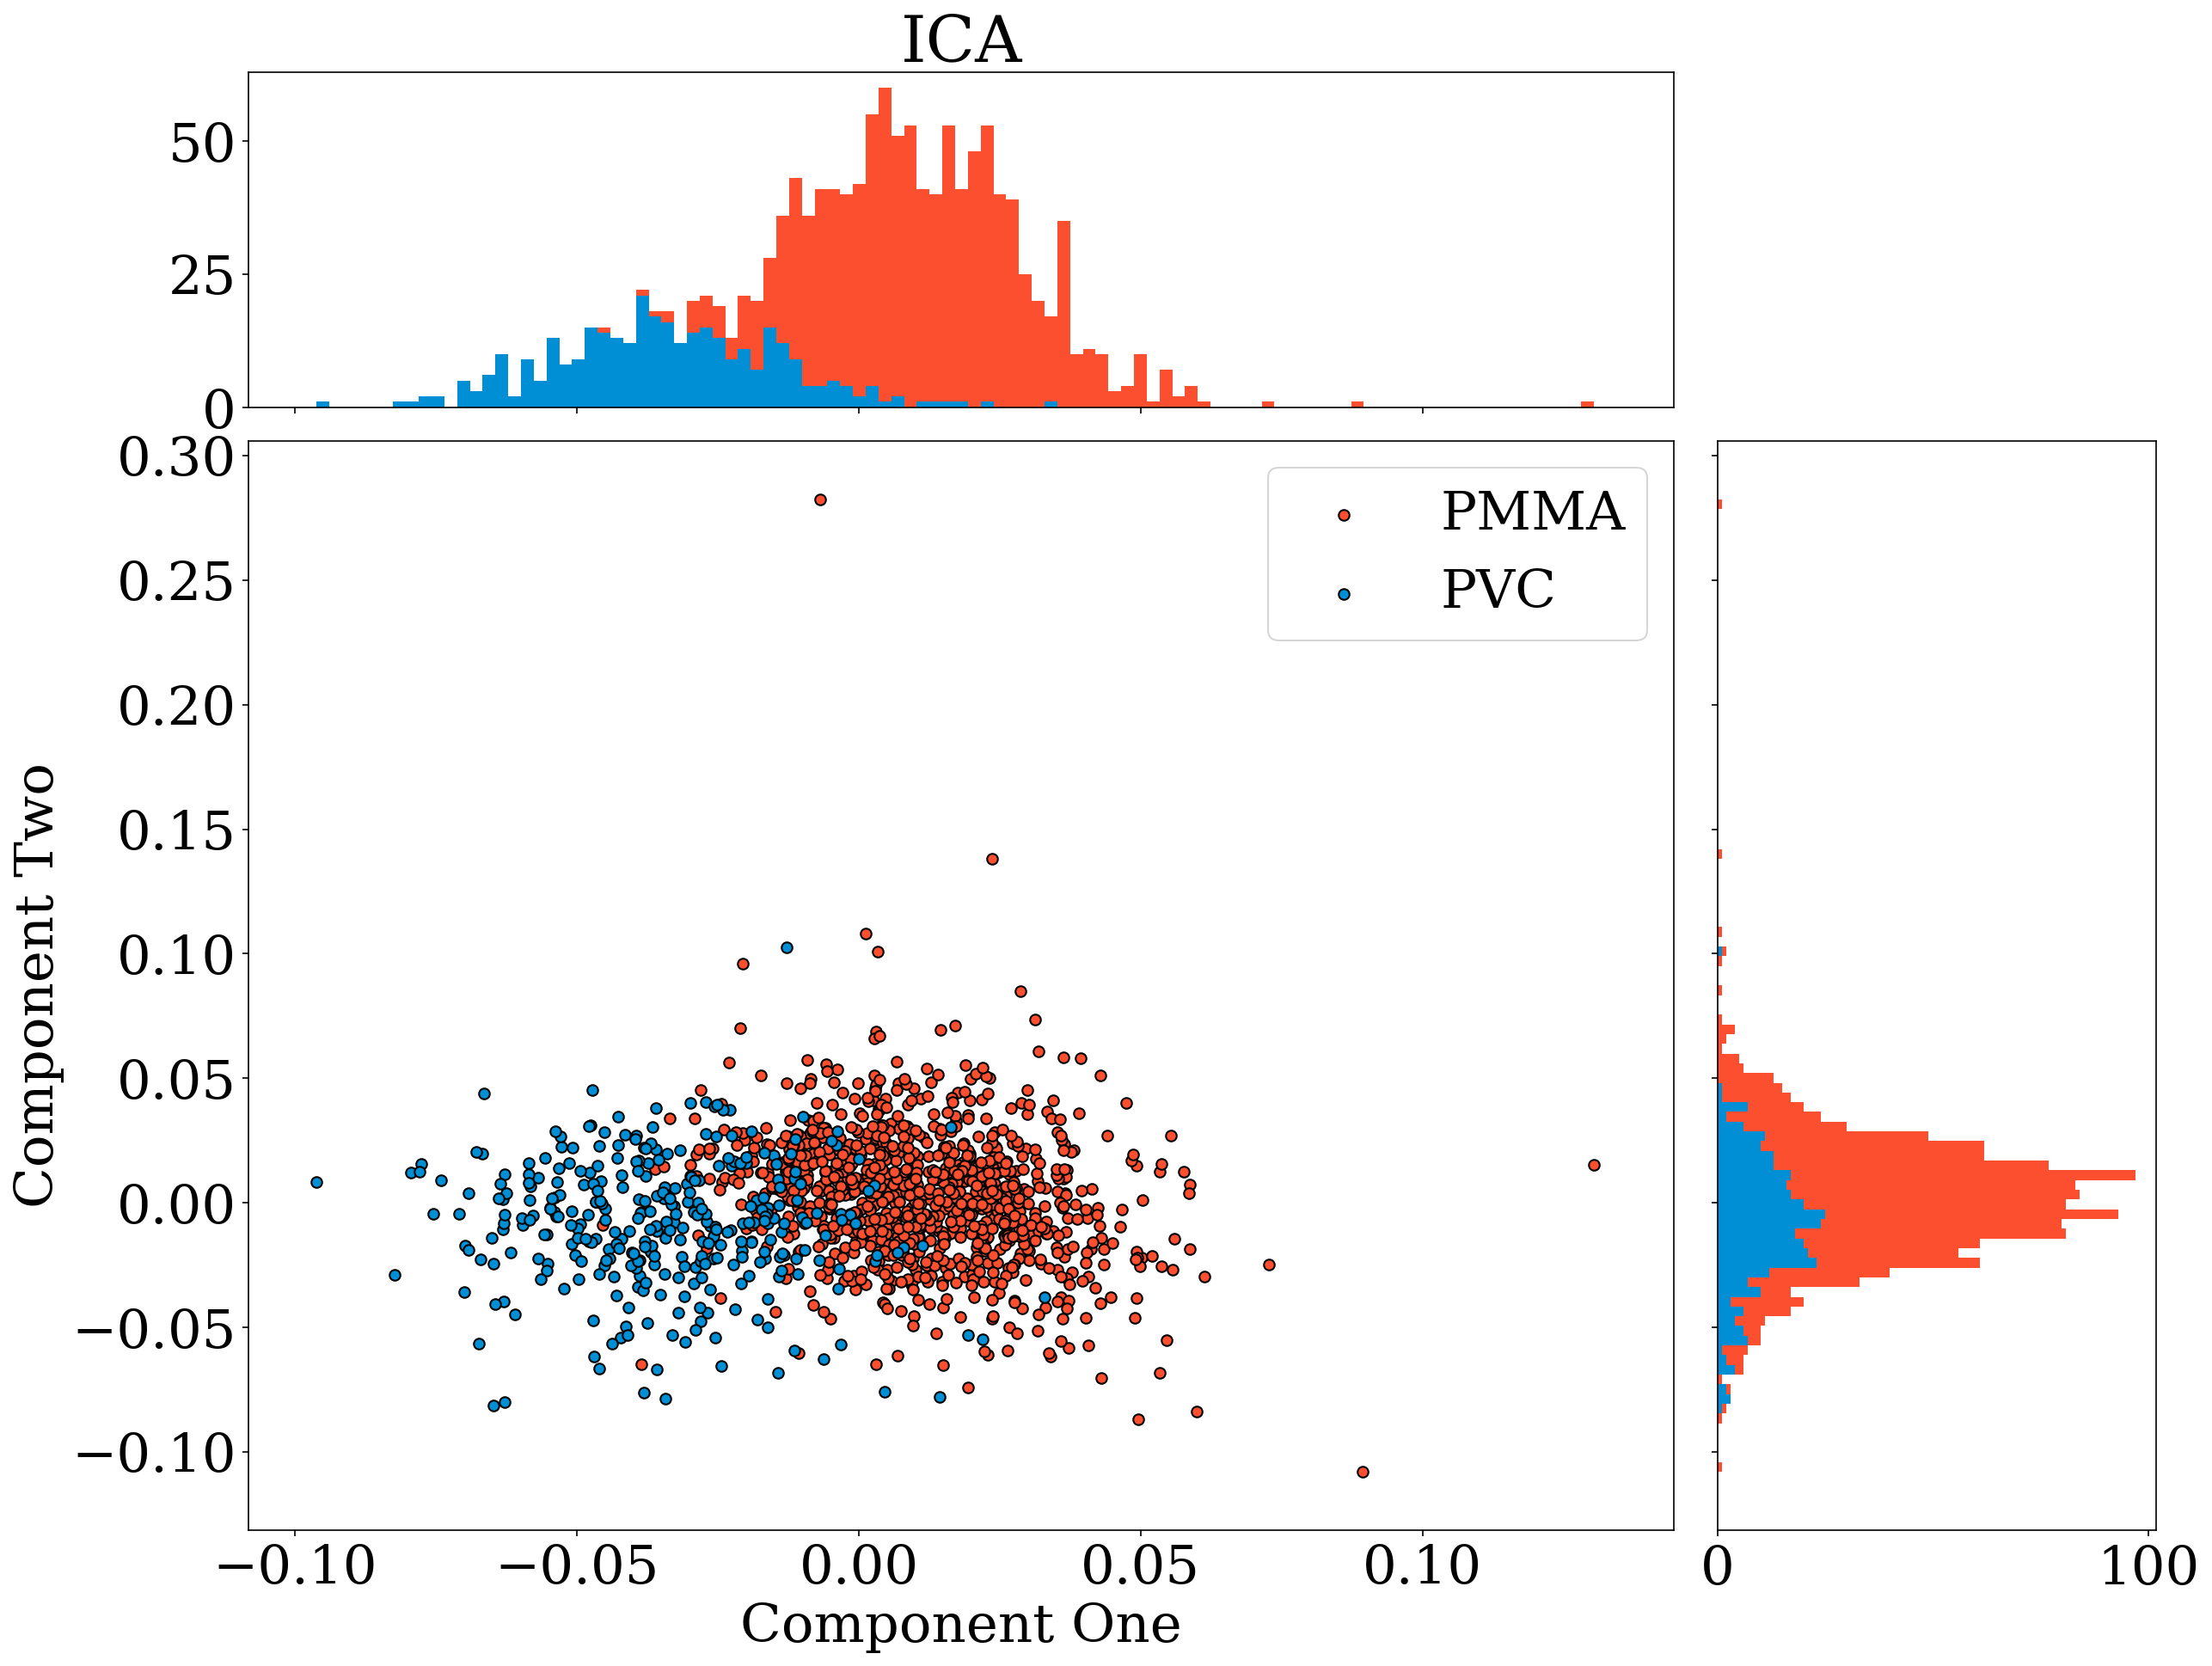
\includegraphics[width=\textwidth]{figures/ICAnone.png}
%     \end{subfigure}
%     ~ %add desired spacing between images, e. g. ~, \quad, \qquad, \hfill etc. 
%     %(or a blank line to force the subfigure onto a new line)
%     \begin{subfigure}[b]{0.3\textwidth}
%         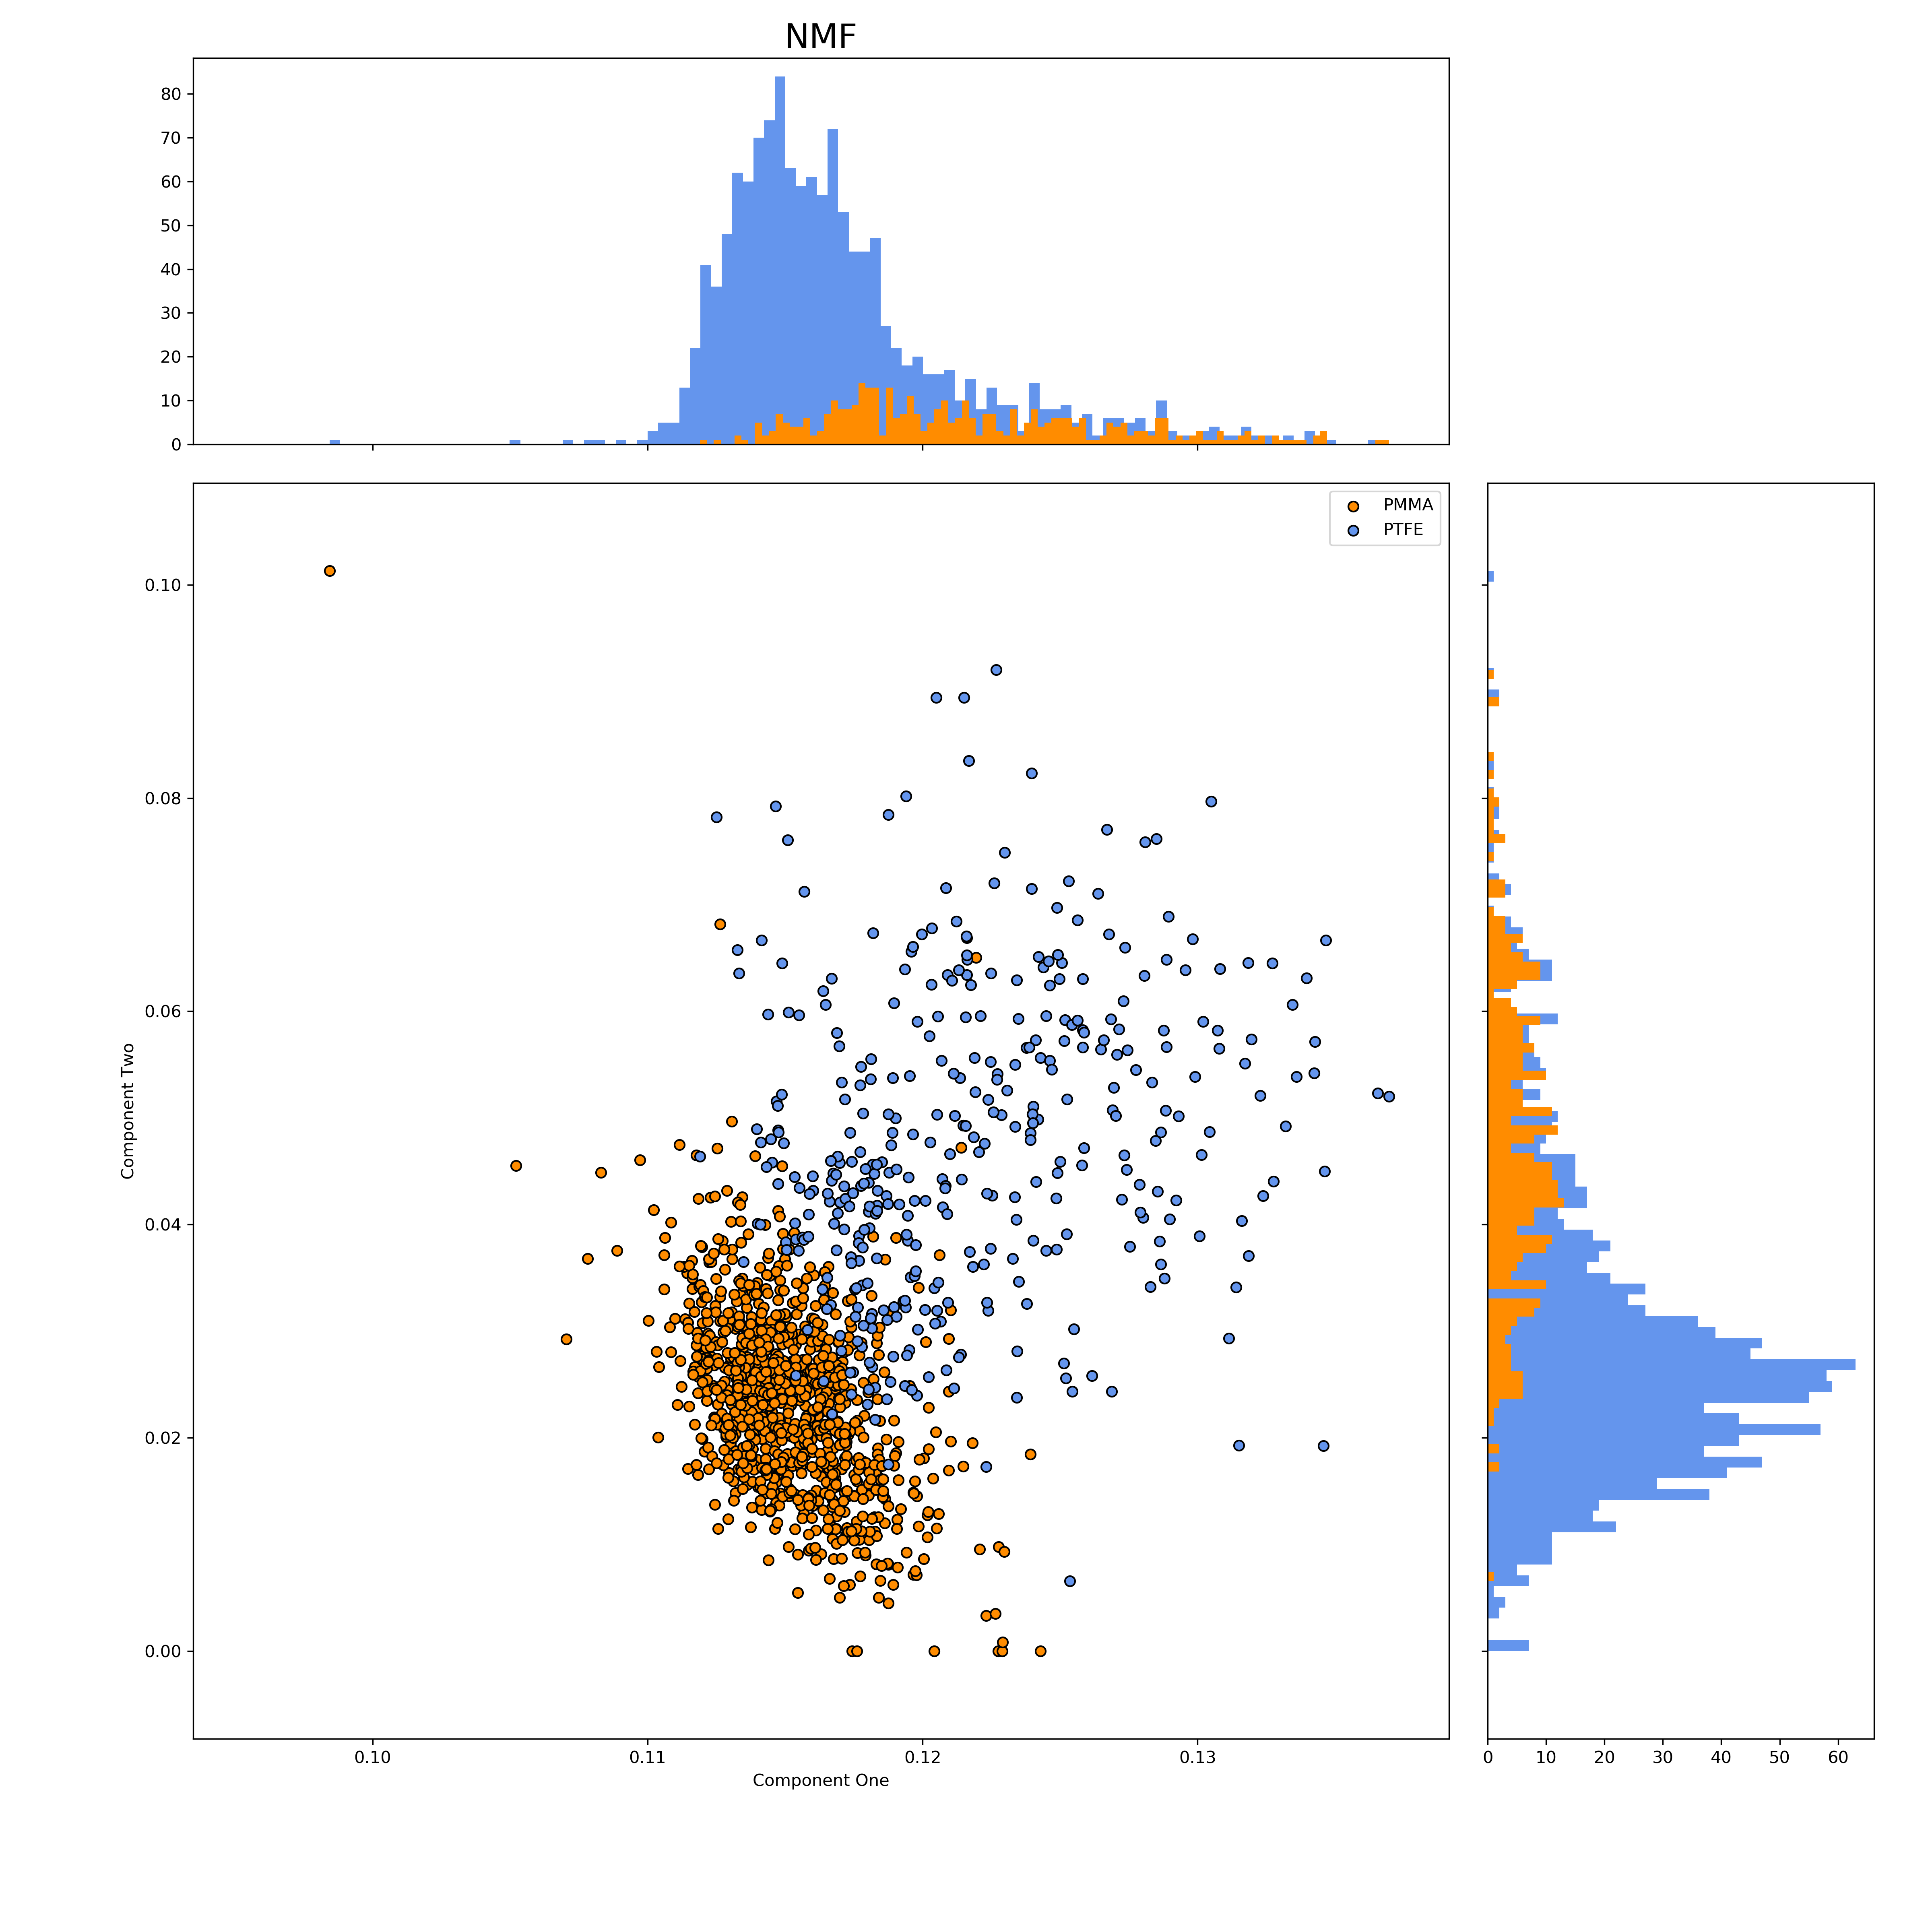
\includegraphics[width=\textwidth]{figures/NMFnone.png}
%     \end{subfigure}
%     \caption{Pictures of animals}\label{dm_methods}
% \end{figure}